%DIF 1-3d1
%DIF LATEXDIFF DIFFERENCE FILE
%DIF DEL main_origin.tex        Fri Jul 24 15:14:27 2026
%DIF ADD main_clean_final.tex   Fri Jul 24 15:14:12 2026
%DIF < % !TeX encoding = UTF-8
%DIF < % !TeX program = pdflatex
%DIF < % IEEEtran Journal Template -- Migrated from Elsevier cja-template.tex
%DIF -------
\documentclass[lettersize,journal]{IEEEtran}

%DIF 6d3
%DIF < %% ---- Packages (only those compatible with IEEEtran) ----
%DIF -------
\usepackage{amsmath,amsfonts,amssymb}
\usepackage{algorithm}
%DIF 9-10c5
%DIF < \usepackage{algorithmic}    % IEEEtran recommends algorithmic (not algorithmicx)
%DIF < \usepackage{array}
%DIF -------
\usepackage{algorithmic}    \usepackage{array} %DIF > 
%DIF -------
\usepackage{bm}
\usepackage{booktabs}
\usepackage{multirow}
\usepackage{graphicx}
%DIF 15a10
\usepackage{placeins} %DIF > 
%DIF -------
\usepackage{url}
%DIF 16-20c12-13
%DIF < \usepackage{cite}           % IEEE-style numeric citations
%DIF < \usepackage{textcomp}
%DIF < \usepackage{stfloats}       % allows figure* at bottom
%DIF < % \usepackage[caption=false,font=normalsize,labelfont=sf,textfont=sf]{subfig}
%DIF < \usepackage[caption=false,font=footnotesize,labelfont=sf,textfont=sf]{subfig}
%DIF -------
\usepackage{cite}           \usepackage{textcomp} %DIF > 
\usepackage{stfloats}       \usepackage[caption=false,font=footnotesize,labelfont=sf,textfont=sf]{subfig} %DIF > 
%DIF -------
\usepackage{siunitx}

%DIF 23d16
%DIF < % theorem/lemma environments
%DIF -------
\newtheorem{theorem}{Theorem}
\newtheorem{lemma}{Lemma}

\hyphenation{op-tical net-works semi-conduc-tor IEEE-Xplore}

%DIF < % ----------------------------------------------------------------
%DIF -------
\graphicspath{{./}{../}{../new_sim_fig/}} %DIF > 
%DIF PREAMBLE EXTENSION ADDED BY LATEXDIFF
%DIF UNDERLINE PREAMBLE %DIF PREAMBLE
\RequirePackage[normalem]{ulem} %DIF PREAMBLE
\RequirePackage{color}\definecolor{RED}{rgb}{1,0,0}\definecolor{BLUE}{rgb}{0,0,1} %DIF PREAMBLE
\providecommand{\DIFadd}[1]{{\protect\color{blue}\uwave{#1}}} %DIF PREAMBLE
\providecommand{\DIFdel}[1]{{\protect\color{red}\sout{#1}}}                      %DIF PREAMBLE
%DIF SAFE PREAMBLE %DIF PREAMBLE
\providecommand{\DIFaddbegin}{} %DIF PREAMBLE
\providecommand{\DIFaddend}{} %DIF PREAMBLE
\providecommand{\DIFdelbegin}{} %DIF PREAMBLE
\providecommand{\DIFdelend}{} %DIF PREAMBLE
\providecommand{\DIFmodbegin}{} %DIF PREAMBLE
\providecommand{\DIFmodend}{} %DIF PREAMBLE
%DIF FLOATSAFE PREAMBLE %DIF PREAMBLE
\providecommand{\DIFaddFL}[1]{\DIFadd{#1}} %DIF PREAMBLE
\providecommand{\DIFdelFL}[1]{\DIFdel{#1}} %DIF PREAMBLE
\providecommand{\DIFaddbeginFL}{} %DIF PREAMBLE
\providecommand{\DIFaddendFL}{} %DIF PREAMBLE
\providecommand{\DIFdelbeginFL}{} %DIF PREAMBLE
\providecommand{\DIFdelendFL}{} %DIF PREAMBLE
\newcommand{\DIFscaledelfig}{0.5}
%DIF HIGHLIGHTGRAPHICS PREAMBLE %DIF PREAMBLE
\RequirePackage{settobox} %DIF PREAMBLE
\RequirePackage{letltxmacro} %DIF PREAMBLE
\newsavebox{\DIFdelgraphicsbox} %DIF PREAMBLE
\newlength{\DIFdelgraphicswidth} %DIF PREAMBLE
\newlength{\DIFdelgraphicsheight} %DIF PREAMBLE
% store original definition of \includegraphics %DIF PREAMBLE
\LetLtxMacro{\DIFOincludegraphics}{\includegraphics} %DIF PREAMBLE
\newcommand{\DIFaddincludegraphics}[2][]{{\color{blue}\fbox{\DIFOincludegraphics[#1]{#2}}}} %DIF PREAMBLE
\newcommand{\DIFdelincludegraphics}[2][]{% %DIF PREAMBLE
\sbox{\DIFdelgraphicsbox}{\DIFOincludegraphics[#1]{#2}}% %DIF PREAMBLE
\settoboxwidth{\DIFdelgraphicswidth}{\DIFdelgraphicsbox} %DIF PREAMBLE
\settoboxtotalheight{\DIFdelgraphicsheight}{\DIFdelgraphicsbox} %DIF PREAMBLE
\scalebox{\DIFscaledelfig}{% %DIF PREAMBLE
\parbox[b]{\DIFdelgraphicswidth}{\usebox{\DIFdelgraphicsbox}\\[-\baselineskip] \rule{\DIFdelgraphicswidth}{0em}}\llap{\resizebox{\DIFdelgraphicswidth}{\DIFdelgraphicsheight}{% %DIF PREAMBLE
\setlength{\unitlength}{\DIFdelgraphicswidth}% %DIF PREAMBLE
\begin{picture}(1,1)% %DIF PREAMBLE
\thicklines\linethickness{2pt} %DIF PREAMBLE
{\color[rgb]{1,0,0}\put(0,0){\framebox(1,1){}}}% %DIF PREAMBLE
{\color[rgb]{1,0,0}\put(0,0){\line( 1,1){1}}}% %DIF PREAMBLE
{\color[rgb]{1,0,0}\put(0,1){\line(1,-1){1}}}% %DIF PREAMBLE
\end{picture}% %DIF PREAMBLE
}\hspace*{3pt}}} %DIF PREAMBLE
} %DIF PREAMBLE
\LetLtxMacro{\DIFOaddbegin}{\DIFaddbegin} %DIF PREAMBLE
\LetLtxMacro{\DIFOaddend}{\DIFaddend} %DIF PREAMBLE
\LetLtxMacro{\DIFOdelbegin}{\DIFdelbegin} %DIF PREAMBLE
\LetLtxMacro{\DIFOdelend}{\DIFdelend} %DIF PREAMBLE
\DeclareRobustCommand{\DIFaddbegin}{\DIFOaddbegin \let\includegraphics\DIFaddincludegraphics} %DIF PREAMBLE
\DeclareRobustCommand{\DIFaddend}{\DIFOaddend \let\includegraphics\DIFOincludegraphics} %DIF PREAMBLE
\DeclareRobustCommand{\DIFdelbegin}{\DIFOdelbegin \let\includegraphics\DIFdelincludegraphics} %DIF PREAMBLE
\DeclareRobustCommand{\DIFdelend}{\DIFOaddend \let\includegraphics\DIFOincludegraphics} %DIF PREAMBLE
\LetLtxMacro{\DIFOaddbeginFL}{\DIFaddbeginFL} %DIF PREAMBLE
\LetLtxMacro{\DIFOaddendFL}{\DIFaddendFL} %DIF PREAMBLE
\LetLtxMacro{\DIFOdelbeginFL}{\DIFdelbeginFL} %DIF PREAMBLE
\LetLtxMacro{\DIFOdelendFL}{\DIFdelendFL} %DIF PREAMBLE
\DeclareRobustCommand{\DIFaddbeginFL}{\DIFOaddbeginFL \let\includegraphics\DIFaddincludegraphics} %DIF PREAMBLE
\DeclareRobustCommand{\DIFaddendFL}{\DIFOaddendFL \let\includegraphics\DIFOincludegraphics} %DIF PREAMBLE
\DeclareRobustCommand{\DIFdelbeginFL}{\DIFOdelbeginFL \let\includegraphics\DIFdelincludegraphics} %DIF PREAMBLE
\DeclareRobustCommand{\DIFdelendFL}{\DIFOaddendFL \let\includegraphics\DIFOincludegraphics} %DIF PREAMBLE
%DIF LISTINGS PREAMBLE %DIF PREAMBLE
\RequirePackage{listings} %DIF PREAMBLE
\RequirePackage{color} %DIF PREAMBLE
\lstdefinelanguage{DIFcode}{ %DIF PREAMBLE
%DIF DIFCODE_UNDERLINE %DIF PREAMBLE
  moredelim=[il][\color{red}\sout]{\%DIF\ <\ }, %DIF PREAMBLE
  moredelim=[il][\color{blue}\uwave]{\%DIF\ >\ } %DIF PREAMBLE
} %DIF PREAMBLE
\lstdefinestyle{DIFverbatimstyle}{ %DIF PREAMBLE
	language=DIFcode, %DIF PREAMBLE
	basicstyle=\ttfamily, %DIF PREAMBLE
	columns=fullflexible, %DIF PREAMBLE
	keepspaces=true %DIF PREAMBLE
} %DIF PREAMBLE
\lstnewenvironment{DIFverbatim}{\lstset{style=DIFverbatimstyle}}{} %DIF PREAMBLE
\lstnewenvironment{DIFverbatim*}{\lstset{style=DIFverbatimstyle,showspaces=true}}{} %DIF PREAMBLE
%DIF END PREAMBLE EXTENSION ADDED BY LATEXDIFF

\begin{document}



%DIF <  ---- Title ----
%DIF <  \title{Multi-Agent Reinforcement Learning-Based Cooperative Interception Strategy
%DIF <    for Maneuvering Swarm Attack Targets with Considering Target Assignment}
\DIFdelbegin %DIFDELCMD < 

%DIFDELCMD < %%%
%DIF <  \title{Trust-Aware Multi-Agent Reinforcement Learning-Based Cooperative Interception Strategy for Maneuvering Swarm Attack Targets Considering Rapid Consensus Target Assignment}
\DIFdelend \title{Trust-Aware Multi-Agent Reinforcement Learning-Based Cooperative Interception Strategy for Maneuvering Swarms with Target Assignment}



%DIF <  ---- Authors ----
%DIF <  \author{Shuyi~Gao,~Defu~Lin,~Duo~Zheng,~and~Zhichen~Chu%
%DIF <  \thanks{S. Gao, D. Lin, D. Zheng, and Z. Chu are with the School of Aerospace
%DIF <  Engineering, Beijing Institute of Technology, Beijing 100081, China
%DIF <  (e-mail: zhengduohello@126.com).}%
%DIF <  \thanks{Manuscript received 2025.}}
\DIFdelbegin %DIFDELCMD < 

%DIFDELCMD < %%%
%DIF < ----双盲投稿--
\DIFdelend \author{}
\DIFdelbegin %DIFDELCMD < \markboth{Under review}%%%
%DIF < 
%DIFDELCMD < {%%%
\DIFdel{Anonymous Submission}%DIFDELCMD < }
%DIFDELCMD < %%%
\DIFdelend \DIFaddbegin \markboth{Under review}{Anonymous Submission}
\DIFaddend 

%DIF <  ---- Running heads ----
\DIFdelbegin %DIFDELCMD < \markboth{IEEE Transactions on Automation Science and Engineering}%%%
%DIF < 
%DIFDELCMD < {%%%
\DIFdel{Gao }%DIFDELCMD < \MakeLowercase{\textit{et al.}}%%%
\DIFdel{: MARL-Based Cooperative Interception for Maneuvering Swarm Targets}%DIFDELCMD < }
%DIFDELCMD < %%%
\DIFdelend \DIFaddbegin \markboth{IEEE Transactions on Automation Science and Engineering}{Gao \MakeLowercase{\textit{et al.}}: MARL-Based Cooperative Interception for Maneuvering Swarm Targets}
\DIFaddend 

\maketitle

%DIF <  ---- Abstract ----
\begin{abstract}
The swarm attack of unmanned aerial vehicles (UAVs) poses a significant threat to future
battlefield operations.
Achieving efficient and precise cooperative interception against attacking UAV swarms with
highly dynamic maneuvering capabilities and adaptive penetration strategies poses a critical
challenge for UAV interceptor swarms.
This study addresses the cooperative interception of maneuvering targets in swarm attacks by
decomposing the problem into two key tasks: target assignment and cooperative interception
guidance.
For target assignment, an Improved Dung Beetle Optimization (IDBO) algorithm is proposed to
dynamically balance exploration and exploitation, achieving highly efficient and rapid
assignments.
%DIF <  For cooperative interception guidance, a multi-agent deep reinforcement learning-based method
%DIF <  is developed to achieve precise and time-coordinated interception of adversarial UAV swarms
%DIF <  employing advanced penetration strategies.
%DIF <  For cooperative interception guidance, a multi-agent deep reinforcement learning framework—augmented by kinematics-aware attention mechanisms and trust-modulated exploration—is developed to achieve precise and time-coordinated interception of adversarial UAV swarms employing advanced penetration strategies.
For cooperative interception guidance, an Attention-Residual and Trust-aware Multi-Agent Proximal Policy Optimization (ART-MAPPO) framework is developed to achieve precise and time-coordinated interception of adversarial UAV swarms employing advanced penetration strategies.
The simulation results validate the effectiveness of the proposed intelligent cooperative
interception method, demonstrating superior convergence speed, robustness, and significantly
improved interception success rates in swarm UAV cooperative interception scenarios.
\end{abstract}

{\linespread{0.9}\selectfont
\hspace*{0.0em}\textbf{\textit{Note to Practitioners—}}\textbf{This paper is motivated by practical UAV swarm defense scenarios, where multiple interceptors must cooperatively engage maneuvering aerial targets under limited communication and onboard maneuver constraints. In such applications, target assignment and guidance are closely coupled, and conventional centralized approaches may be difficult to implement efficiently as the engagement scale increases. To address this issue, this paper develops a two-stage cooperative interception framework that combines distributed target assignment with a trust-aware multi-agent reinforcement learning guidance method. The proposed approach is intended to improve coordination consistency among interceptors assigned to the same target and to enhance robustness against target maneuvers while considering maneuver saturation and command smoothness. This work may be useful for practical large-scale multi-UAV interception and other cooperative autonomous systems requiring scalable distributed decision-making and coordinated guidance.}\par\vspace{0.5\baselineskip}
}

%DIF <  ---- Keywords ----
\begin{IEEEkeywords}
Cooperative interception, deep reinforcement learning, centralized training with decentralized
execution, target assignment, UAV swarm.
\end{IEEEkeywords}


%DIF < % ===========================================================
\section{Introduction}
\label{sec:introduction}
\IEEEPARstart{A}{s} warfare evolves toward intelligent swarm operations, the likelihood of
encountering attacks from adversarial UAV swarms significantly increases during combat.
Consequently, the efficient interception of incoming swarm targets becomes a critical
imperative for future battlefield operations.
To address the challenge of cooperative interception against maneuvering attacking swarms with
adaptive penetration strategies, there is an urgent need to advance academic research in swarm
target interception technologies.
This study aims to enhance interceptors with intelligent cooperative interception capabilities,
enabling effective navigation of complex challenges in modern battlefield environments.

Multi-target cooperative interception encompasses two key tasks: target assignment and
cooperative interception.
The effectiveness of multi-target interception hinges on the optimality of target assignment,
establishing it as a primary focus in swarm target interception strategies.
As the number of UAVs increases, the complexity of target assignment escalates significantly,
resulting in a multi-constrained, multi-parameter optimization problem.
The objective is to develop a rapid and efficient target assignment method for allocating
specific attacking targets to interceptors in operational scenarios~\cite{KLINE2019226}.
The target assignment problem involves complex constraints, and the non-dominated sorting
algorithm can dynamically generate a set of reference points with good convergence and
distribution performance~\cite{WANG2025952,bai2024hybrid,zou2024moea}.
Moreover, employing an online operator selection mechanism can enhance the efficiency of the
algorithm~\cite{ahmad2024fuzzy,ming2024constrained}.
The target assignment problem can be solved using multi-information particle swarm optimization
to find the solution that yields the highest gain~\cite{mishra2015weapon,wei2020particle}.
Introducing information from surrounding particles can enhance the stability of the traditional
particle swarm algorithm while also addressing the issue of local convergence in the target
assignment problem~\cite{long2024improved}.
The genetic algorithm is a common approach for solving the target assignment
problem~\cite{he4914655modelling,li2020multi,sun2022multi,chang2018solving}, and a GA with a
novel crossover operator can further enhance algorithmic efficiency~\cite{weng2024diversity}.
Ant colony optimization is also an effective strategy for solving the target assignment
problem~\cite{li2024comprehensive}, and its combination with a greedy algorithm can improve
the accuracy of parallel computation~\cite{yi2024solving}.
Under multiple constraints, researchers have proposed various heuristic algorithms to solve the
target assignment problem, such as neural networks~\cite{li2024comprehensive}, auction
algorithm~\cite{wang2024collaborative}, tabu search~\cite{yao2024tabu}, simulated annealing
algorithm~\cite{khurshid2024hybrid}, VLSN~\cite{yue2024graph}.
However, in cooperative interception scenarios, the aforementioned algorithms struggle to
handle the highly dynamic nature of the battlefield due to their high time complexity, and they
fail to meet the dual requirements of both speed and optimality.

The effectiveness of the terminal guidance phase in multi-target interception is significantly
influenced by the cooperative guidance law, a critical factor requiring thorough consideration.
The target assignment strategy transforms swarm operations into a coordinated multi-to-one
interception problem, with current research focusing on three key areas: angular coordination,
temporal coordination, and intelligent cooperation.
Significant progress has been made in temporal coordination.
Classical proportional navigation-based guidance laws enable synchronized multi-missile attacks
on a single target~\cite{tao2024analytical}.
Adaptive control methods adjust attack timing based on real-time operational conditions, making
them suitable for intercepting maneuvering targets~\cite{wang2025generalized,zhang2022multiple}.
Sliding Mode Control (SMC) is widely adopted for cooperative
interception~\cite{sinha2020supertwisting}, with SMC incorporating miss distance and attack
time constraints enhancing interception
accuracy~\cite{shen2025three,jin2025cooperative,hu2019sliding}.
Considerable research has also been conducted on angular coordination.
From a traditional control perspective, backstepping control~\cite{li2024adaptive} and
leader-follower cooperative methods~\cite{he2017impact} significantly improve interception
efficiency.
SMC with angular constraints is prevalent in cooperative interception, encompassing approaches
based on impact angle constraints~\cite{wang2025hybrid} and line-of-sight angle
constraints~\cite{li2024near}.
Optimal control methods applied to impact angle-constrained cooperative guidance enhance
precision by integrating impact angle and line-of-sight angle
constraints~\cite{wang2025adaptive,tao2023optimal}.

Recent advancements in intelligent technologies have driven extensive research into cooperative
interception strategies for UAV swarms, with intelligent algorithms demonstrating substantial
potential in addressing complex multi-target scenarios~\cite{chen2024enhanced,wu2020collaborative}.
Optimization-based approaches, such as Particle Swarm Optimization (PSO), excel in
collaborative attack problems by autonomously optimizing resource allocation and maximizing
operational efficiency~\cite{zhao2024hierarchical,wu2020collaborative}.
Search-based algorithms, like A*~\cite{liao2024research}, enable efficient path planning for
coordinated attacks.
Control-based methods, including Model Predictive Control
(MPC)~\cite{kim2024adaptive}, provide robust guidance under dynamic constraints.
Moreover, the integration of neural networks with reinforcement learning, particularly deep
reinforcement learning (DRL), enhances the adaptability and intelligence of interception
strategies~\cite{luo2022uav,zhan2022multiple,wang2021uav}.
DRL enables UAV swarms to learn complex policies from high-dimensional data, optimizing target
assignment and maneuvering in real-time to counter maneuvering targets~\cite{sun2024memory}.
In contrast, conventional cooperative interception guidance methods rely heavily on
linearization and simplifying assumptions to design feasible guidance laws~\cite{zhao2025global}.
These methods often struggle to address the complexity of dynamic, non-linear environments
involving maneuvering swarm targets.
Data-driven intelligent cooperative interception methods, by contrast, leverage extensive
datasets to learn adaptive strategies, significantly reducing dependence on restrictive
assumptions~\cite{fainkich2025cooperative}.
By modeling complex interactions through neural networks and DRL, these methods achieve greater
robustness and flexibility.
Despite advancements, intelligent cooperative interception methods struggle with maneuvering
swarm targets in complex dynamic environments due to limited model generalization, low training
efficiency, and low interception success rates, particularly in large-scale swarm combat
requiring precise temporal coordination~\cite{horyna2023decentralized}.
Addressing these challenges requires further research into scalable, generalizable, and
efficient algorithms to fully realize the potential of intelligent cooperative interception.

In summary, existing cooperative interception methods for countering attacking UAV swarms with
adaptive penetration capabilities suffer from low interception success rates in complex dynamic
environments.
Specifically, target assignment methods exhibit low allocation efficiency, while cooperative
interception guidance strategies struggle with terminal overload saturation and insufficient
adaptability to dynamic target maneuvers in practical scenarios, hindering effective swarm
coordination.
Consequently, more research is necessary to address these challenges.

This study proposes a swarm cooperative interception method based on multi-agent reinforcement
learning and IDBO algorithm, enhancing target assignment efficiency and guidance strategy
performance to achieve precise and efficient interception of maneuvering targets.
The proposed intelligent cooperative interception algorithm offers the following advantages.

\begin{enumerate}
\item A distributed consensus-based target assignment scheme is proposed, which integrates an
improved Dung Beetle Optimization (IDBO) algorithm with a combat-dominance assessment model.
This design supports rapid many-to-one allocation under limited communication, leading to more
efficient and reliable target assignment for cooperative interception.

\item ART-MAPPO is proposed as a CTDE-based cooperative interception guidance learning
framework, which employs an attention--residual feature extractor and a GRU temporal encoder,
and \DIFdelbegin \DIFdel{integrates }\DIFdelend \DIFaddbegin \DIFadd{uses }\DIFaddend trust-modulated exploration \DIFdelbegin \DIFdel{with a }\DIFdelend \DIFaddbegin \DIFadd{together with }\DIFaddend dual-clip PPO \DIFdelbegin \DIFdel{update }\DIFdelend and adaptive KL
regularization \DIFaddbegin \DIFadd{for stable policy learning}\DIFaddend . This design \DIFdelbegin \DIFdel{yields faster convergence and improved }\DIFdelend \DIFaddbegin \DIFadd{improves convergence behavior and
}\DIFaddend training efficiency in highly maneuverable swarm-adversarial environments.

\item A \DIFdelbegin \DIFdel{cooperative interception method augmented with a reinforcement learning-based reward function is introduced, enabling precise temporal coordination. This strategy enhances
interception success rates against }\DIFdelend \DIFaddbegin \DIFadd{task-oriented reward design and training stabilization strategy are incorporated into
the cooperative interception framework to support time-coordinated guidance under bounded
overload commands. Rather than treating reward shaping or dual-clip PPO as standalone
methodological novelties, this work uses them as task-adapted components that couple target
approach, terminal interception, temporal coordination, and control-effort regularization in a
}\DIFaddend large-scale maneuvering swarm \DIFdelbegin \DIFdel{targets by addressing dynamic
coordination challenges}\DIFdelend \DIFaddbegin \DIFadd{scenario}\DIFaddend .
\end{enumerate}

The paper is structured as follows: Section~\ref{sec:method} presents relevant problem modeling and foundational theory. Section~\ref{sec:target_assignment} and Section~\ref{sec:cooperative_algorithm} provide a detailed description of our approach, including its framework, modules, algorithms, and rationale. Section~\ref{sec:simulation} covers experiments, results, and discussions. Lastly, Section~\ref{sec:conclusion} summarizes the paper and outlines future directions.

%DIF < % ===========================================================
\section{Backgrounds and Preliminaries}
\label{sec:method}

In this section, we first introduce the modeling of multi-target interception of UAVs, and
then review reinforcement learning methods.

\subsection{Problem Modeling}

The multi-target intelligent interception problem can be decomposed into two subproblems:
target assignment and intelligent cooperative interception, with the swarm combat scenario
illustrated in Fig.~\ref{fenpei}.
In this scenario, the attacking swarm aims to penetrate a high-value target area, while the
defending swarm seeks to fully intercept the incoming UAVs.
During the target assignment phase, the defending swarm assesses its own flight status and
that of the attacking swarm using onboard sensors, subsequently allocating each defender to an
appropriate interception target via the target assignment strategy.
In the intelligent cooperative interception phase, defenders assigned to the same target employ
coordinated maneuvering strategies to intercept and neutralize the target.

\begin{figure}[!t]
\centering
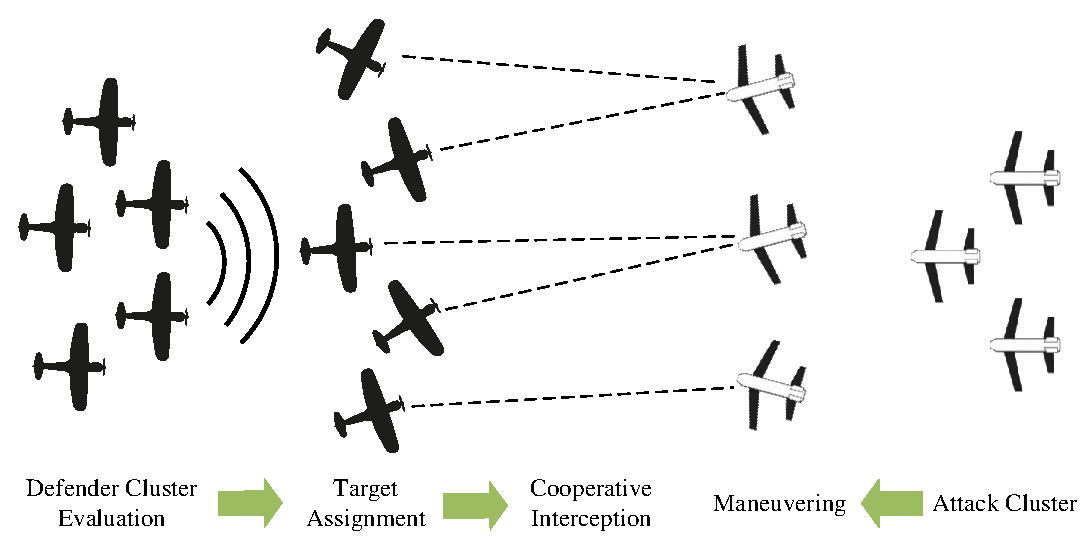
\includegraphics[width=2.8in]{fenpei.pdf}
\caption{Cluster target interception problem.}
\label{fenpei}
\end{figure}

The object of study in this paper is the fixed-wing UAV\DIFdelbegin \DIFdel{, and the interception problem is
reduced to a two-dimensional horizontal plane as shown in }\DIFdelend \DIFaddbegin \DIFadd{. }\DIFaddend Fig.~\ref{jianmo} \DIFdelbegin \DIFdel{without loss of
generality}\DIFdelend \DIFaddbegin \DIFadd{shows the
horizontal projection used to define the heading and line-of-sight (LOS) azimuth, whereas the
guidance model and simulations propagate the complete three-dimensional position and velocity}\DIFaddend .

\begin{figure}[!t]
\centering
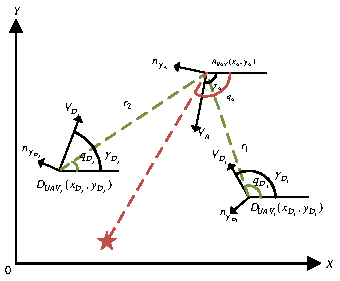
\includegraphics[width=2.6in]{pic02.pdf}
\caption{Schematic diagram of confrontation and interception.}
\label{jianmo}
\end{figure}

The \DIFaddbegin \DIFadd{three-dimensional point-mass }\DIFaddend kinematic model of a single UAV \DIFdelbegin \DIFdel{can be simplified as
}\begin{displaymath}
\DIFdel{%DIFDELCMD < \label{yundongxue}%%%
\left\{\begin{matrix}\dot{x} =V\cos\gamma \\
\dot{y} =V\sin\gamma \end{matrix}\right.
}\end{displaymath}%DIFAUXCMD
\DIFdelend \DIFaddbegin \DIFadd{is
}\begin{equation}
\DIFadd{\label{yundongxue}
\left\{\begin{aligned}
\dot{x}&=V\cos\theta\cos\gamma,\\
\dot{y}&=V\cos\theta\sin\gamma,\\
\dot{z}&=V\sin\theta,
\end{aligned}\right.
}\end{equation}\DIFaddend 
where \DIFdelbegin \emph{\DIFdel{x}}%DIFAUXCMD
\DIFdelend \DIFaddbegin \DIFadd{$(x,y,z)$ are the three-dimensional position coordinates}\DIFaddend , \DIFdelbegin \emph{\DIFdel{y}} %DIFAUXCMD
\DIFdel{is the position coordinates of the UAV in two-dimensional space, }\emph{\DIFdel{V}} %DIFAUXCMD
\DIFdelend \DIFaddbegin \DIFadd{$V$ }\DIFaddend is the velocity
magnitude\DIFdelbegin \DIFdel{of the UAV, and $\gamma$ is the navigation }\DIFdelend \DIFaddbegin \DIFadd{, $\gamma$ is the heading angle, and $\theta$ is the flight-path (pitch) }\DIFaddend angle.

In an interception mission, \DIFdelbegin \DIFdel{the relative motion relationship between the attacking and defending UAVs can be described as:
}\begin{displaymath}
\DIFdel{%DIFDELCMD < \label{gongfang}%%%
\left\{\begin{matrix}\dot{r} =V_{A}\cos(\gamma_{A}-q)-V_{D}\cos(\gamma_{D}-q) \\
r\dot{q} =V_{A}\sin(\gamma_{A}-q)-V_{D}\sin(\gamma_{D}-q)\end{matrix}\right.
}\end{displaymath}%DIFAUXCMD
\DIFdelend \DIFaddbegin \DIFadd{let $\mathbf p_A,\mathbf p_D\in\mathbb R^3$ and
$\mathbf v_A,\mathbf v_D\in\mathbb R^3$ denote the attacker and defender states. Their
three-dimensional relative geometry is
}\begin{equation}
\DIFadd{\label{gongfang}
\begin{aligned}
\mathbf r_{AD}&=\mathbf p_A-\mathbf p_D,\qquad
r=\|\mathbf r_{AD}\|_2,\\
\boldsymbol\ell_{AD}&=\mathbf r_{AD}/r,\qquad
\dot r=\boldsymbol\ell_{AD}^{\top}(\mathbf v_A-\mathbf v_D).
\end{aligned}
}\end{equation}\DIFaddend 
\DIFdelbegin \DIFdel{where }\DIFdelend \DIFaddbegin \DIFadd{Here, }\DIFaddend $r$ is the \DIFaddbegin \DIFadd{three-dimensional }\DIFaddend inter-UAV distance \DIFdelbegin \DIFdel{, $q$ is the line-of-sight angle, $V_{A}$ ($V_{D}$) is the
velocity of the attacking (defending) UAV, and
$\gamma_{A}$ ($\gamma_{D}$) is the corresponding heading angle}\DIFdelend \DIFaddbegin \DIFadd{and
$\boldsymbol\ell_{AD}$ is the LOS unit vector; its horizontal projection provides the
plan-view geometry shown in Fig.~\ref{jianmo}}\DIFaddend .

\DIFdelbegin \DIFdel{In the interception phase, the relationship between UAV }\DIFdelend \DIFaddbegin \DIFadd{The relationship between the }\DIFaddend flight state and \DIFdelbegin \DIFdel{acceleration is
:
}\begin{displaymath}
\DIFdel{%DIFDELCMD < \label{guozai}%%%
\left\{\begin{matrix}\dot{V} =n_{x} g \\
\dot{\gamma} =n_{y}g/V \end{matrix}\right.
}\end{displaymath}%DIFAUXCMD
\DIFdelend \DIFaddbegin \DIFadd{the three commanded load channels is
}\begin{equation}
\DIFadd{\label{guozai}
\left\{\begin{aligned}
\dot V&=n_xg,\\
\dot\gamma&=\frac{n_yg}{V\cos\theta},\\
\dot\theta&=\frac{n_zg}{V},
\end{aligned}\right.
}\end{equation}\DIFaddend 
where \DIFdelbegin \DIFdel{$n_{x}$ }\DIFdelend \DIFaddbegin \DIFadd{$n_x$ }\DIFaddend is the axial \DIFdelbegin \DIFdel{acceleration command, $n_{y}$ is the normal acceleration command}\DIFdelend \DIFaddbegin \DIFadd{load-factor command, $n_y$ and $n_z$ are the horizontal and vertical
normal load-factor commands, respectively}\DIFaddend , and $g$ is \DIFdelbegin \DIFdel{the }\DIFdelend gravitational acceleration. \DIFaddbegin \DIFadd{Thus,
$n_y$ primarily changes heading, while $n_z$ changes the flight-path angle and altitude.
}\DIFaddend In the multi-agent setting of Section~\ref{sec:cooperative_algorithm}, these variables carry
an agent subscript $i$.

During cooperative interception, the remaining impact time is defined as:
\begin{equation}
\label{shijian}
t_{go}=\frac{r}{\left|\dot{r}\right|}
\end{equation}

The \DIFaddbegin \DIFadd{three-dimensional }\DIFaddend Zero-Effort Miss (ZEM) is defined as
\DIFdelbegin \DIFdel{:
}\begin{displaymath}
\DIFdel{%DIFDELCMD < \label{ZEM}%%%
ZEM = \frac{r^{2}\cdot\dot{q}}{\left|\dot{r}\right|}
}\end{displaymath}%DIFAUXCMD
\DIFdelend \DIFaddbegin \begin{equation}
\DIFadd{\label{ZEM}
\operatorname{ZEM}=\left\|\mathbf r_{AD}
+(\mathbf v_A-\mathbf v_D)t_{go}\right\|_2.
}\end{equation}\DIFaddend 

\subsection{Reinforcement Learning}

Reinforcement learning (RL) is built on the Markov Decision Process (MDP), comprising state
space $\mathcal{S}$, action space $\mathcal{A}$, reward function $R$, policy $\pi$, and state
transition function $P$.
At each step, the agent selects action $a$ from state $s$, receives reward $r$, and
transitions to $s'$.
The key value functions are:
\begin{equation}
\label{RLV}
V^{\pi}(s)=E_{\pi}\left[\sum_{t=0}^{\infty}\gamma_{\mathrm{RL}}^{t}r_{t}\mid s_{0}=s\right]
\end{equation}
\begin{equation}
\label{RLQ}
Q^{\pi}(s,a)=E_{\pi}\left[\sum_{t=0}^{\infty}\gamma_{\mathrm{RL}}^{t}r_{t}\mid s_{0}=s,a_{0}=a\right]
\end{equation}
where $\gamma_{\mathrm{RL}}\in[0,1]$ is the discount factor.






\section{Target Assignment via Distributed Consensus-Based IDBO Algorithm}
\label{sec:target_assignment}

This section formulates \DIFdelbegin \DIFdel{the }\DIFdelend cooperative target assignment as a \DIFdelbegin \DIFdel{weighted }\DIFdelend \DIFaddbegin \DIFadd{capacitated }\DIFaddend bipartite matching
problem and \DIFdelbegin \DIFdel{solves it via an Improved Dung Beetle Optimization (IDBO ) algorithm embedded in a
distributed consensus framework. }%DIFDELCMD < 

%DIFDELCMD < %%%
\subsection{\DIFdel{Problem Formulation}}
%DIFAUXCMD
\addtocounter{subsection}{-1}%DIFAUXCMD
%DIFDELCMD < \label{subsec:problem_formulation}
%DIFDELCMD < 

%DIFDELCMD < %%%
\DIFdel{Let $\mathcal{U} = \{u_1, u_2, \dots, u_M\}$ and
$\mathcal{T} = \{t_1, t_2, \dots, t_N\}$ denote the interceptor }\DIFdelend \DIFaddbegin \DIFadd{then describes how local IDBO search and neighbor-to-neighbor bidding produce a
consistent many-to-one assignment. To avoid overloading the notation used later for learning,
let $\mathcal{D}=\{d_1,\ldots,d_{N_D}\}$ and
$\mathcal{T}=\{t_1,\ldots,t_{N_A}\}$ denote the defender }\DIFaddend and target sets, respectively\DIFdelbegin \DIFdel{. Figure }\DIFdelend \DIFaddbegin \DIFadd{;
$i$ always indexes a defender and $j$ a target in this section.
}

\subsection{\DIFadd{Pairwise Interception Model and Assignment Objective}}
\label{subsec:problem_formulation}

\DIFadd{Figure~}\DIFaddend \ref{km} illustrates the bipartite assignment structure. \DIFdelbegin %DIFDELCMD < 

%DIFDELCMD < \begin{figure}[!t]
%DIFDELCMD < \centering
%DIFDELCMD < 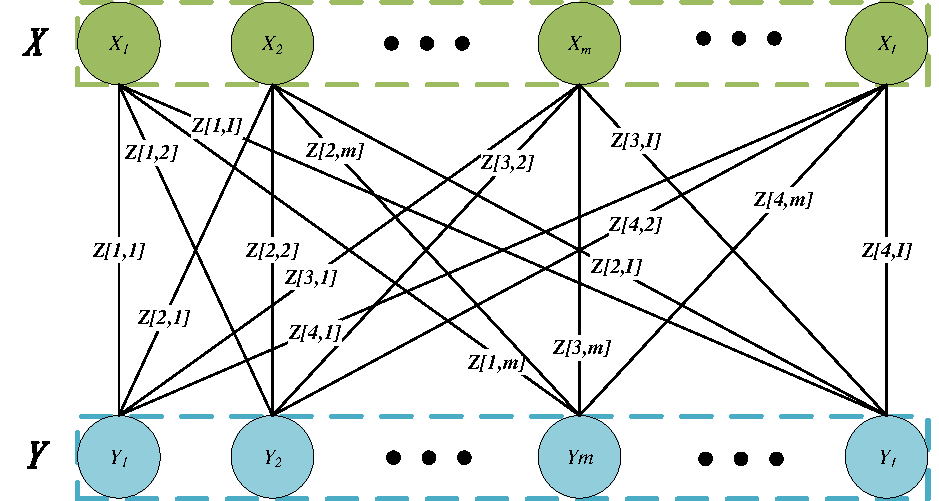
\includegraphics[width=2.5in]{KM1.pdf}
%DIFDELCMD < %%%
%DIFDELCMD < \caption{%
{%DIFAUXCMD
\DIFdelFL{Schematic diagram of weighted dichotomy.}}
%DIFAUXCMD
%DIFDELCMD < \label{km}
%DIFDELCMD < \end{figure}
%DIFDELCMD < 

%DIFDELCMD < %%%
\DIFdel{The binary decision }\DIFdelend \DIFaddbegin \DIFadd{The binary }\DIFaddend variable
$X_{ij}=1$ \DIFdelbegin \DIFdel{if UAV $u_i$ }\DIFdelend \DIFaddbegin \DIFadd{indicates that defender $d_i$ }\DIFaddend is assigned to target $t_j$\DIFdelbegin \DIFdel{and 0 otherwise. The edge weight $P_{ij}$ quantifies the interception probability:
}%DIFDELCMD < 

%DIFDELCMD < %%%
\begin{displaymath}
\DIFdel{
P_{ij} = w_1 \cdot P_{\text{ZEM}}(i,j) + w_2 \cdot P_{\sigma}(i,j)
}\end{displaymath}%DIFAUXCMD
\DIFdel{where $w_1 + w_2 = 1$, $w_1, w_2 \geq 0$. The Zero-Effort Miss (ZEM) component is :
}%DIFDELCMD < 

%DIFDELCMD < %%%
\begin{displaymath}
\DIFdel{
P_{\text{ZEM}}(i,j) = \exp\left[-\frac{1}{2}\left(\frac{\text{ZEM}(i,j)}{\overline{\text{ZEM}}}\right)^2\right]
}\end{displaymath}%DIFAUXCMD
\DIFdel{where $\overline{\text{ZEM}} = \frac{1}{MN}\sum_{i=1}^{M}\sum_{j=1}^{N} \text{ZEM}(i,j)$.
}%DIFDELCMD < 

%DIFDELCMD < %%%
\DIFdel{The angular advantage component is:
}%DIFDELCMD < 

%DIFDELCMD < %%%
\begin{displaymath}
\DIFdel{
P_{\sigma}(i,j) = \exp\left[-\frac{1}{2}\left(\frac{S_{\sigma}(i,j)}{\overline{S_{\sigma}}}\right)^2\right]
}\end{displaymath}%DIFAUXCMD
\DIFdelend \DIFaddbegin \DIFadd{. A useful edge should
simultaneously have a small predicted miss tendency and a favorable heading geometry. We
therefore define the pairwise interception-probability proxy as
}\begin{equation}
\DIFadd{\label{eq:pair_score}
\begin{aligned}
p_{ij}^{\mathrm{int}}
 &= \omega_Z\exp\!\left[-\frac{1}{2}
       \left(\frac{\mathrm{ZEM}_{ij}}{s_Z}\right)^2\right]
  + \omega_{\ell}\exp\!\left[-\frac{1}{2}
       \left(\frac{e_{ij}^{\ell}}{s_{\ell}}\right)^2\right],\\
e_{ij}^{\ell}
 &= \arccos\!\left(\operatorname{clip}\!\left(
 \frac{\mathbf v_{D_i}^{\mathsf T}\boldsymbol\ell_{ij}}{\|\mathbf v_{D_i}\|_2+\varepsilon_{\mathrm{num}}},-1,1\right)\right),
\end{aligned}
}\end{equation}\DIFaddend 
where \DIFdelbegin \DIFdel{$\overline{S_{\sigma}} = \frac{1}{MN}\sum_{i=1}^{M}\sum_{j=1}^{N} S_{\sigma}(i,j)$, with $S_{\sigma}(i,j) = |\gamma_{ij} - q_{ij}|$ denoting the heading error. The objective minimizes the expected number of surviving targets. Under many-to-one assignment, the joint survival probability of target $t_j$ is
}\DIFdelend \DIFaddbegin \DIFadd{$s_Z=[(N_DN_A)^{-1}\sum_{i,j}\mathrm{ZEM}_{ij}^{2}]^{1/2}
+\varepsilon_{\mathrm{num}}$ and
$s_{\ell}=[(N_DN_A)^{-1}\sum_{i,j}(e_{ij}^{\ell})^{2}]^{1/2}
+\varepsilon_{\mathrm{num}}$ are root-mean-square normalization scales. Here,
$\boldsymbol\ell_{ij}=(\mathbf p_{T_j}-\mathbf p_{D_i})/
\|\mathbf p_{T_j}-\mathbf p_{D_i}\|_2$ is }\DIFaddend the \DIFdelbegin \DIFdel{product of individual failure probabilities:
}%DIFDELCMD < 

%DIFDELCMD < %%%
\begin{displaymath}
\DIFdel{
\begin{aligned}
\min_{\mathbf{X}} \quad & J = \sum_{j=1}^{N} \left[ \prod_{i=1}^{M} \left(1 - P_{ij}\right)^{X_{ij}} \right] \\
\text{s.t.} \quad & \sum_{j=1}^{N} X_{ij} = 1, \quad \forall i \in \{1,\dots,M\} \\
& \sum_{i=1}^{M} X_{ij} \geq 1, \quad \forall j \in \{1,\dots,N\} \\
& \sum_{i=1}^{M} X_{ij} \leq L_{\max}, \quad \forall j \in \{1,\dots,N\} \\
& X_{ij} \in \{0,1\}, \quad \forall i,j
\end{aligned}
}\end{displaymath}%DIFAUXCMD
\DIFdel{where $\prod_{i=1}^{M} (1 - P_{ij})^{X_{ij}}$ yields the survival probability of $t_j$, which decreases geometrically with the number of assigned interceptors}\DIFdelend \DIFaddbegin \DIFadd{three-dimensional line-of-sight unit vector,
and $\operatorname{clip}(\cdot,-1,1)$ keeps the inverse-cosine argument numerically valid.
The nonnegative weights satisfy $\omega_Z+\omega_{\ell}=1$.
Thus, either a large predicted miss or poor velocity-to-LOS alignment reduces the edge value,
whereas a geometrically favorable
pair has $p_{ij}^{\mathrm{int}}$ close to one. The RMS scales avoid cancellation of signed
ZEM values and make the two terms comparable. In implementation, this bounded quantity is
used as a probability proxy; the product model below adopts the usual conditional-independence
approximation for different defenders assigned to the same target}\DIFaddend .

\DIFdelbegin \subsection{\DIFdel{Distributed Consensus-Based IDBO Framework}}
%DIFAUXCMD
\addtocounter{subsection}{-1}%DIFAUXCMD
%DIFDELCMD < \label{subsec:idbo_algorithm}
%DIFDELCMD < %%%
\DIFdelend \DIFaddbegin \begin{figure}[!t]
\centering
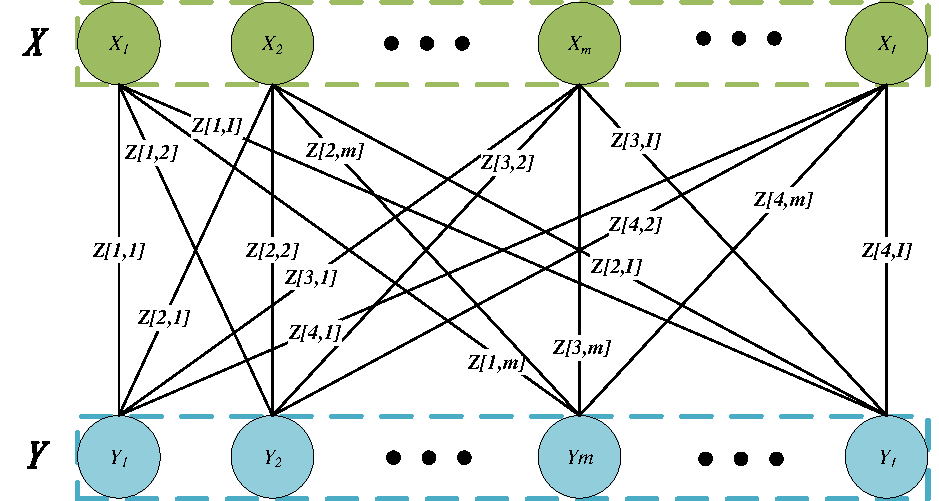
\includegraphics[width=2.5in]{KM1.pdf}
\caption{\DIFaddFL{Bipartite representation of defender--target assignment.}}
\label{km}
\end{figure}
\DIFaddend 

The \DIFdelbegin \DIFdel{IDBO algorithm solves }%DIFDELCMD < \eqref{eq:optimization_formulation} %%%
\DIFdel{by alternating between local metaheuristic optimization and distributed consensus-based conflict resolution. Let $\mathbf{X}^{(k)} = [x_{ij}^{(k)}] \in \{0,1\}^{M \times N}$ denote the assignment matrix at iteration $k$, where $x_{ij}^{(k)}=1$ indicates UAV $u_i$ is assigned }\DIFdelend \DIFaddbegin \DIFadd{tactical objective is to reduce the expected number of surviving targets. Assigning an
additional capable defender }\DIFaddend to target $t_j$ \DIFdelbegin \DIFdel{. }\DIFdelend \DIFaddbegin \DIFadd{multiplies its approximate survival probability
by another failure factor. The resulting capacitated assignment is
}\begin{equation}
\DIFadd{\label{eq:optimization_formulation}
\begin{aligned}
\min_{\mathbf X}\quad
&J(\mathbf X)=\sum_{j=1}^{N_A}\prod_{i=1}^{N_D}
       \left(1-p_{ij}^{\mathrm{int}}\right)^{X_{ij}}\\
\mathrm{s.t.}\quad
&\sum_{j=1}^{N_A}X_{ij}=1, && i=1,\ldots,N_D,\\
&1\leq\sum_{i=1}^{N_D}X_{ij}\leq L_{\max},
&&j=1,\ldots,N_A,\\
&X_{ij}\in\{0,1\}.&&
\end{aligned}
}\end{equation}
\DIFaddend The \DIFdelbegin \DIFdel{integrated optimization is
:
}\DIFdelend \DIFaddbegin \DIFadd{first constraint assigns every defender to exactly one target; the second prevents both
uncovered targets and excessive concentration. A feasible assignment requires
$N_A\leq N_D\leq L_{\max}N_A$.
}\DIFaddend 

\DIFdelbegin \begin{displaymath}
\DIFdel{%DIFDELCMD < %%%
\mathcal{A}_{\text{IDBO}}^{(k+1)} = \mathcal{G}_{\text{consensus}} \circ \mathcal{F}_{\text{optimizer}} \left( \mathbf{X}^{(k)}, \boldsymbol{\Theta}^{(k)} \right)
}\end{displaymath}%DIFAUXCMD
\DIFdel{where $\mathcal{F}_{\text{optimizer}}$ denotes the improved DBO operator and $\mathcal{G}_{\text{consensus}}$ the consensus-based conflict resolver. The parameter set $\boldsymbol{\Theta}^{(k)} = \{\mathbf{A}^{(k)}, \mathbf{P}^{(k)}, \mathbf{V}^{(k)}\}$ aggregates the adversarial advantage, interception probability, and velocity matrices at iteration $k$}\DIFdelend \DIFaddbegin \subsection{\DIFadd{Local IDBO Search and Consensus Bidding}}
\label{subsec:idbo_algorithm}

\DIFadd{The distributed solution alternates between two interpretable operations. Each defender first
searches for a promising target using locally available engagement information; neighboring
defenders then reconcile conflicting choices by exchanging target-specific bids. Defender
$d_i$ maintains an unconstrained preference vector
$\boldsymbol{\xi}_i\in\mathbb{R}^{N_A}$ and maps it to soft preferences
$\pi_{ij}=\sigma(\xi_{ij})$, where $\sigma(x)=(1+e^{-x})^{-1}$. This separates the
continuous search variable $\xi_{ij}$ from the binary assignment variable $X_{ij}$}\DIFaddend .

\DIFdelbegin \DIFdel{Each UAV $u_i$ maintains a preference vector $\mathbf{x}_i \in [0,1]^{N}$, where $x_{ij}$ encodes the
normalized affinity for }\DIFdelend \DIFaddbegin \DIFadd{For }\DIFaddend target $t_j$\DIFdelbegin \DIFdel{. The fitness function balances interception efficiency against resource saturation:
}%DIFDELCMD < 

%DIFDELCMD < %%%
\begin{displaymath}
\DIFdel{
\begin{split}
\mathcal{F}_i(\mathbf{x}_i) =& \sum_{j=1}^{N} \sigma(x_{ij}) \cdot P_{ij} + \lambda_1 \sum_{j=1}^{N} \sigma(x_{ij}) \cdot A_{ij} \\
&- \lambda_2 \sum_{j=1}^{N} \Psi_{ij}(\mathbf{x}_i, \hat{\mathbf{X}}_{\mathcal{N}_i})
\end{split}
}\end{displaymath}%DIFAUXCMD
\DIFdel{where the three terms correspond to interception probability, adversarial advantage($\lambda_1$-weighted), and an over-saturation penalty ($\lambda_2$-weighted). The penalty $\Psi_{ij}$ is:
}%DIFDELCMD < 

%DIFDELCMD < %%%
\begin{displaymath}
\DIFdel{
\begin{split}
\Psi_{ij}(\mathbf{x}_i, \hat{\mathbf{X}}_{\mathcal{N}_i}) =& \sigma(x_{ij}) \cdot \max\Biggl(0, \Biggl(\sum_{k \in \mathcal{N}_i, k \neq i} \sigma(\hat{x}_{kj}) \\
&+ \sigma(x_{ij})\Biggr) - L_{\max}\Biggr)
\end{split}
}\end{displaymath}%DIFAUXCMD
\DIFdelend \DIFaddbegin \DIFadd{, let $\widehat n_{ij}=\sum_{\ell\in\mathcal N_i\setminus\{i\}}
\widehat\pi_{\ell j}$ be the assignment load estimated from defender $d_i$'s neighbor set
$\mathcal N_i$. The target-specific utility and aggregate local fitness are
}\begin{equation}
\DIFadd{\label{eq:local_utility}
\begin{aligned}
u_{ij}(\boldsymbol\xi_i)
 &=\pi_{ij}\bigl(p_{ij}^{\mathrm{int}}+\lambda_A\chi_{ij}\bigr)
 -\lambda_L\pi_{ij}
   \left[\widehat n_{ij}+\pi_{ij}-L_{\max}\right]_{+},\\
\mathcal F_i(\boldsymbol\xi_i)&=\sum_{j=1}^{N_A}u_{ij}(\boldsymbol\xi_i),
\end{aligned}
}\end{equation}\DIFaddend 
where \DIFdelbegin \DIFdel{$\mathcal{N}_i$ }\DIFdelend \DIFaddbegin \DIFadd{$[x]_{+}=\max(0,x)$ and $\chi_{ij}$ }\DIFaddend is the \DIFdelbegin \DIFdel{neighbor set of $u_i$, $\hat{x}_{kj}$ the
estimated preference of neighbor $u_k$, and $L_{\max}$ the per-target interceptor capacity . The penalty activates only when the estimated assignment count exceeds $L_{\max}$, steering the swarm toward capacity-feasible solutions}\DIFdelend \DIFaddbegin \DIFadd{combat advantage}\DIFaddend . \DIFdelbegin %DIFDELCMD < 

%DIFDELCMD < %%%
\DIFdelend The \DIFdelbegin \DIFdel{adversarial advantage $A_{ij}$ fuses temporal, energetic, and geometric factors:
}\DIFdelend \DIFaddbegin \DIFadd{first term favors
interceptable and tactically advantageous targets; the hinge term is inactive below the
estimated capacity and increases only when another defender would oversubscribe that target.
}\DIFaddend 

\DIFdelbegin \begin{displaymath}
\DIFdel{
\begin{split}
A_{ij} =& \exp\left(-\frac{\Delta t_{ij}}{T_{\max}}\right) \cdot \left(1 - \frac{\|\mathbf{v}_i - \mathbf{v}_j\|_2}{v_{\max}}\right) \\
&\cdot \max\left(0, \cos(\theta_{ij})\right) - \sum_{k\neq i} \frac{P_{kj}}{P_{ij} + P_{kj}} \cdot \sigma(\hat{x}_{kj})
\end{split}
}\end{displaymath}%DIFAUXCMD
\DIFdelend \DIFaddbegin \DIFadd{The advantage combines time, relative-velocity compatibility, encounter geometry, and local
competition:
}\begin{equation}
\DIFadd{\label{eq:adversarial_advantage}
\begin{aligned}
\chi_{ij}={}&
\exp\!\left(-\frac{\Delta t_{ij}}{T_c}\right)
\left[1-\frac{\|\mathbf v_{D_i}-\mathbf v_{T_j}\|_2}{v_c}\right]_{+}
\left[\cos(\vartheta_{ij})\right]_{+}\\
&-\lambda_C\!\sum_{\ell\in\mathcal N_i\setminus\{i\}}
\frac{p_{\ell j}^{\mathrm{int}}}{p_{ij}^{\mathrm{int}}+p_{\ell j}^{\mathrm{int}}+\varepsilon_{\mathrm{num}}}
\widehat\pi_{\ell j}.
\end{aligned}
}\end{equation}\DIFaddend 
\DIFdelbegin \DIFdel{where }\DIFdelend \DIFaddbegin \DIFadd{Here, }\DIFaddend $\Delta t_{ij}$ is the estimated \DIFdelbegin \DIFdel{time-to-intercept; $\mathbf{p}_i=[x_i, y_i]^\top$ and $\mathbf{v}_i=[\dot{x}_i, \dot{y}_i]^\top$ denote the position and velocity vectors of interceptor $u_i$; $\mathbf{p}_j=[x_j, y_j]^\top$ and $\mathbf{v}_j=[\dot{x}_j, \dot{y}_j]^\top$ denote the position and velocity vectors of target $t_j$; $\theta_{ij}$ is the aspect angle associated with the engagement geometry between $u_i$ and $t_j$; and $v_{\max}$ is the maximum reference speed used for normalization . The three multiplicative factors encode temporal, energetic, and geometric advantage, respectively, while the subtracted term penalizes competition from other interceptors with high preferences for the same target }\DIFdelend \DIFaddbegin \DIFadd{intercept time, $\vartheta_{ij}$ is the encounter
aspect angle, and $T_c$ and $v_c$ are positive normalization constants. The positive-part
operators prevent a large relative-speed mismatch or an unfavorable aspect angle from
producing a negative multiplicative ``advantage.'' The final term lowers the utility of a
target already preferred by capable neighbors}\DIFaddend .

\DIFdelbegin \DIFdel{The IDBO update mechanism enhances the standard DBO through four adversarial-information-driven operations :
}%DIFDELCMD < 

%DIFDELCMD < %%%
\begin{align*}
\DIFdel{\text{Rolling:} \quad }& \DIFdel{\mathbf{x}_i^{(t+1)} = \mathbf{x}_i^{(t)} + \alpha \cdot \nabla_{\mathbf{x}_i} \mathcal{F}_i(\mathbf{x}_i^{(t)}) \circ \mathbf{A}_i \nonumber }\\
& \DIFdel{\quad + \beta \cdot \mathbf{r}_i \cdot \exp\left(-\frac{t}{T}\right)  }\\
\DIFdel{\text{Dancing:} \quad }& \DIFdel{\mathbf{x}_i^{(t+1)} = \mathbf{x}_i^{(t)} \odot \exp\left(\gamma \cdot \tanh(\mathbf{A}_i - \bar{A}_i)\right) \nonumber }\\
& \DIFdel{\quad + \mathbf{n}_i, \quad \mathbf{n}_i \sim \mathcal{N}(0, \sigma_d^2 \mathbf{I})  }\\
\DIFdel{\text{Breeding:} \quad }& \DIFdel{\mathbf{x}_i^{(t+1)} = \mathbf{x}_i^{(t)} + \delta \cdot \left(\mathbf{x}_{\text{best}}^{(t)} - \mathbf{x}_i^{(t)}\right) \odot \mathbf{A}_i \nonumber }\\
& \DIFdel{\quad + \delta' \cdot \left(\mathbf{x}_{\text{second}}^{(t)} - \mathbf{x}_i^{(t)}\right)  }\\
\DIFdel{\text{Stealing:} \quad }& \DIFdel{\mathbf{x}_i^{(t+1)} = \mathbf{x}_i^{(t)} \nonumber }\\
& \DIFdel{\quad + \eta \cdot \sum_{k \in \mathcal{K}_i} \frac{A_{ij}}{\sum_{l \in \mathcal{K}_i} A_{lj}} \cdot \left(\mathbf{x}_k^{(t)} - \mathbf{x}_i^{(t)}\right) 
}\end{align*}%DIFAUXCMD
\DIFdelend \DIFaddbegin \DIFadd{Rather than presenting four long update equations in succession, we collect the rolling,
dancing, breeding, and stealing operations into one implementation operator:
}\begin{equation}
\DIFadd{\label{eq:idbo_update}
\boldsymbol\xi_i^{(k+1)}=
\Pi_{\Xi}\!\left[
\mathcal U_{\mathrm{IDBO}}
\bigl(\boldsymbol\xi_i^{(k)},\mathcal F_i,
      \boldsymbol\chi_i^{(k)};k\bigr)\right].
}\end{equation}\DIFaddend 
\DIFdelbegin \DIFdel{where $\mathbf{A}_i = [A_{i1}, A_{i2}, \dots, A_{iN}]^\top$, $\bar{A}_i$ is the mean of $\mathbf{A}_i$, $\mathbf{r}_i$ and $\mathbf{n}_i$ are random vectors, $\mathcal{K}_i$ represents UAVs competing for the same targets as $u_i$, and $\alpha, \beta, \gamma, \delta, \delta', \eta$ are adaptive coefficients that decay linearly with iteration $t$.
Continuous preferences are binarized via advantage-adaptive thresholding:
}\DIFdelend \DIFaddbegin \DIFadd{The four operations respectively perform local exploitation, controlled perturbation, elite
recombination, and preference exchange. Their coefficients decay with assignment iteration
$k$, so early iterations explore broadly and later iterations refine high-utility candidates.
$\Pi_{\Xi}$ clips the latent preferences to their numerical search bounds after every update.
The procedural order and feasibility repair are stated explicitly in Algorithm~\ref{alg:idbo};
the compact form in }\eqref{eq:idbo_update} \DIFadd{keeps the main physical flow visible.
}\DIFaddend 

\DIFdelbegin \begin{displaymath}
\DIFdel{%DIFDELCMD < %%%
X_{ij} = 
\begin{cases}
1, & \text{if } \sigma(x_{ij}) > \tau \cdot \left(1 + \frac{A_{ij}}{\max_k A_{ik}}\right) \\
0, & \text{otherwise}
\end{cases}
}\end{displaymath}%DIFAUXCMD
\DIFdelend \DIFaddbegin \DIFadd{After local search, defender $d_i$ selects exactly one candidate target,
}\begin{equation}
\DIFadd{\label{eq:candidate_assignment}
\widetilde X_{ij}^{(k+1)}=
\mathbb I\!\left[j=\underset{r\in\{1,\ldots,N_A\}}{\arg\max}
u_{ir}(\boldsymbol\xi_i^{(k+1)})\right],
}\end{equation}\DIFaddend 
\DIFdelbegin \DIFdel{where $\tau \in (0,1)$ is a base threshold.
Each UAV maintains a bundle $\mathcal{B}_i$, bid vector $\mathbf{c}_i = [c_{i1}, \dots, c_{iN}]$,
winner list $\mathbf{z}_i = [z_{i1}, \dots, z_{iN}]$, and timestamp vector $\mathbf{y}_i = [y_{i1}, \dots, y_{iN}]$. The bid for target $t_j$ governs the distributed auction:
}%DIFDELCMD < 

%DIFDELCMD < %%%
\begin{displaymath}
\DIFdel{
c_{ij} = \mathcal{F}_i(\mathbf{x}_i) \cdot \sigma(x_{ij}) \cdot \exp\left(\frac{A_{ij} - \bar{A}_i}{\sigma_A}\right)
}\end{displaymath}%DIFAUXCMD
\DIFdelend \DIFaddbegin \DIFadd{with deterministic index-based tie breaking. Unlike independent thresholding, this mapping
cannot return either zero targets or multiple targets for one defender. The corresponding bid
amplifies targets for which the defender has an above-average combat advantage:
}\begin{equation}
\DIFadd{\label{eq:bid_formulation}
b_{ij}^{(k+1)}=\widetilde X_{ij}^{(k+1)}u_{ij}
\exp\!\left(\frac{\chi_{ij}-\bar\chi_i}{s_{\chi,i}+\varepsilon_{\mathrm{num}}}\right),
}\end{equation}\DIFaddend 
where \DIFdelbegin \DIFdel{$\bar{A}_i$ and $\sigma_A$ }\DIFdelend \DIFaddbegin \DIFadd{$\bar\chi_i$ and $s_{\chi,i}$ }\DIFaddend are the mean and standard deviation of
\DIFdelbegin \DIFdel{$u_i$'s adversarial advantages. The fitness--preference product captures local assignment quality, while the exponential term amplifies bids for targets where $u_i$ holds above-average advantage. To support cooperative saturation attacks, the consensus mechanism employs top-$K$ bidding.
Each UAV maintains a winner list $\mathcal{Z}_{j} = \{(u_k, c_{kj})\}$ for $t_j$, containing up to $L_{\max}$ highest bids:
}%DIFDELCMD < 

%DIFDELCMD < %%%
\begin{displaymath}
\DIFdel{
\mathcal{Z}_{j}^{(k+1)} = \text{Top}_{L_{\max}} \left( \mathcal{Z}_{j}^{(k)} \cup \bigcup_{l \in \mathcal{N}_i} \mathcal{Z}_{j,l}^{(k)} \cup \{(u_i, c_{ij}^{(k+1)})\} \right)
}\end{displaymath}%DIFAUXCMD
\DIFdel{where $\text{Top}_{L_{\max}}(\cdot)$ retains the $L_{\max}$ highest-bid entries. UAV $u_i$ secures a slot for $t_j$ if $|\mathcal{Z}_{j}| < L_{\max}$ or its bidexceeds $\min_{(u_k, c_{kj}) \in \mathcal{Z}_{j}} c_{kj}$, thereby displacing the weakest contributor and prioritizing the most capable interceptors.
}%DIFDELCMD < 

%DIFDELCMD < %%%
\DIFdel{As depicted in the procedural flowchart (Fig. ~\ref{fig:idbo_flowchart}), the algorithm iterates over three interleaved phases—local optimization (Eqs.~\ref{eq:rolling_update}--\ref{eq:stealing_update}), consensus resolution (Eqs.~\ref{eq:thresholding}--\ref{eq:cbba_update}), and advantage update—until convergence:
}%DIFDELCMD < 

%DIFDELCMD < %%%
\begin{align*}
\DIFdel{\text{Phase 1: } }& \DIFdel{\mathbf{x}_i^{(k+1)} = \mathcal{F}_{\text{optimizer}}\left(\mathbf{x}_i^{(k)}, \mathcal{F}_i, \mathbf{A}_i^{(k)}, \mathbf{P}^{(k)}\right)  }\\
\DIFdel{\text{Phase 2: } }& \DIFdel{\{\mathbf{z}_i^{(k+1)}, \mathcal{B}_i^{(k+1)}\} = \nonumber }\\ 
& \DIFdel{\mathcal{G}_{\text{consensus}}\left(\{\sigma(\mathbf{x}_i^{(k+1)})\}, \{\mathbf{c}_i^{(k+1)}\}, \{\mathbf{y}_i^{(k)}\}\right)  }\\
\DIFdel{\text{Phase 3: } }& \DIFdel{\mathbf{A}_i^{(k+1)} = \mathcal{H}\left(\mathbf{z}_i^{(k+1)}, \mathcal{B}_i^{(k+1)}, \mathbf{V}_i^{(k+1)}, \mathbf{V}_T^{(k+1)}\right) %DIFDELCMD < %%%
}\end{align*}%DIFAUXCMD
\DIFdelend \DIFaddbegin \DIFadd{$\{\chi_{ij}\}_{j=1}^{N_A}$.
}

\DIFadd{Each defender stores a local winner set $\mathcal W_{i,j}$ for every target. After receiving
neighbor copies, it retains the highest $L_{\max}$ bids:
}\begin{equation}
\DIFadd{\label{eq:cbba_update}
\mathcal W_{i,j}^{(k+1)}=\operatorname{Top}_{L_{\max}}
\left(\mathcal W_{i,j}^{(k)}
\cup\!\bigcup_{\ell\in\mathcal N_i}\mathcal W_{\ell,j}^{(k)}
\cup\{(d_i,b_{ij}^{(k+1)})\}\right).
}\end{equation}\DIFaddend 
\DIFaddbegin \DIFadd{Because only the selected target receives a nonzero bid, the winner sets enforce the target
capacity without destroying the one-target-per-defender interpretation. A defender displaced
from a full winner set removes that target from its local candidate and searches/bids again in
the next iteration.
}\DIFaddend 

\begin{figure}[!t]
\centering
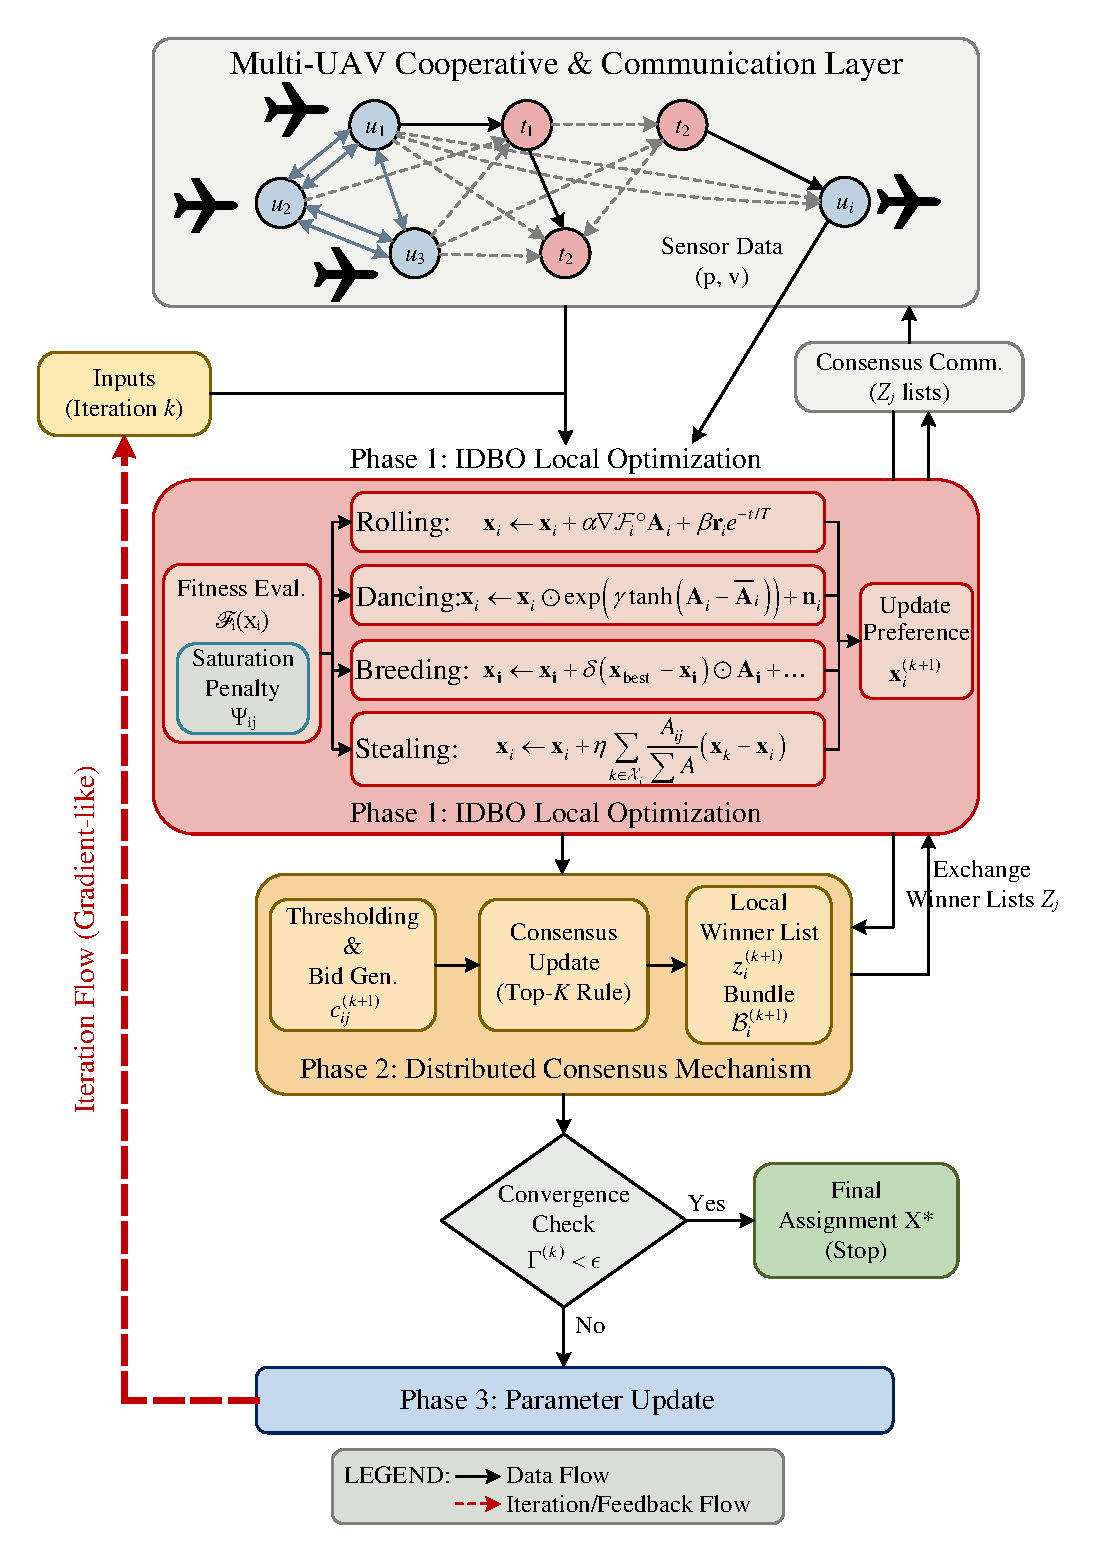
\includegraphics[width=3.2in]{assignment.pdf}
\caption{\DIFdelbeginFL \DIFdelFL{Flowchart of the distributed consensus-based }\DIFdelendFL \DIFaddbeginFL \DIFaddFL{Distributed }\DIFaddendFL IDBO \DIFdelbeginFL \DIFdelFL{algorithm, illustrating the algorithmic iteration }\DIFdelendFL \DIFaddbeginFL \DIFaddFL{assignment }\DIFaddendFL flow\DIFdelbeginFL \DIFdelFL{across }\DIFdelendFL \DIFaddbeginFL \DIFaddFL{: }\DIFaddendFL local \DIFdelbeginFL \DIFdelFL{metaheuristic optimization}\DIFdelendFL \DIFaddbeginFL \DIFaddFL{preference search}\DIFaddendFL , \DIFdelbeginFL \DIFdelFL{auction-based }\DIFdelendFL \DIFaddbeginFL \DIFaddFL{one-hot candidate
selection, top-$L_{\max}$ }\DIFaddendFL consensus \DIFaddbeginFL \DIFaddFL{bidding}\DIFaddendFL , and \DIFdelbeginFL \DIFdelFL{adversarial information updates}\DIFdelendFL \DIFaddbeginFL \DIFaddFL{engagement-information update}\DIFaddendFL .}
\label{fig:idbo_flowchart}
\end{figure}

\DIFdelbegin \DIFdel{Here, $\mathcal{H}$ updates adversarial advantages given the consensus assignment and velocity vectors $\mathbf{V}_i$, $\mathbf{V}_T$. Following the iteration flow in Fig. ~\ref{fig:idbo_flowchart}, convergence is declared when the swarm-wide assignment disagreement falls below $\epsilon$:
}%DIFDELCMD < 

%DIFDELCMD < %%%
\begin{displaymath}
\DIFdel{%DIFDELCMD < %%%
\Gamma^{(k)} = \frac{1}{M} \sum_{i=1}^{M} \left\| \mathbf{z}_i^{(k)} - \frac{1}{|\mathcal{N}_i|} \sum_{j \in \mathcal{N}_i} \mathbf{z}_j^{(k)} \right\|_0 < \epsilon
}\end{displaymath}%DIFAUXCMD
\DIFdel{where $\|\cdot\|_0$ counts disagreeing entries and $\epsilon$ is a convergence threshold.
The algorithm guarantees monotonic fitness improvement: $\Phi^{(k+1)} \geq \Phi^{(k)}$ a
.s., where $\Phi^{(k)} = \sum_{i=1}^{M} \mathcal{F}_i(\mathbf{x}_i^{(k)})$. Under a connected communication graph with finitemessage delays, consensus }\DIFdelend \DIFaddbegin \DIFadd{Let $\mathbf W_i^{(k)}=\{\mathcal W_{i,j}^{(k)}\}_{j=1}^{N_A}$ and let
$\mathcal E$ denote the communication edges. The normalized pairwise disagreement }\DIFaddend is
\DIFdelbegin \DIFdel{reached in at most $N \cdot D$ iterations ($D$: graph diameter). The converged assignment $\mathbf{X}^*$ constitutes an
$\epsilon$-approximate Nash equilibrium: $\mathcal{F}_i(\mathbf{x}_i^*) \geq \mathcal{F}_i(\mathbf{x}_i') - \epsilon$, $\forall \mathbf{x}_i' \in \mathcal{X}_i$}\DIFdelend \DIFaddbegin \begin{equation}
\DIFadd{\label{eq:convergence}
\Gamma^{(k)}=\frac{1}{|\mathcal E|}
\sum_{(i,\ell)\in\mathcal E}
\mathbb I\!\left[\mathbf W_i^{(k)}\neq\mathbf W_{\ell}^{(k)}\right]
\leq\varepsilon_{\mathrm{con}}.
}\end{equation}
\DIFadd{This definition directly counts communication links whose winner information is inconsistent;
it is zero when all neighboring defenders agree.
}

\subsection{\DIFadd{Convergence Scope and Computational Cost}}
\label{subsec:convergence_equilibrium}

\DIFadd{The convergence statement concerns agreement of the distributed assignment process for a
fixed engagement snapshot, not global optimality of the nonconvex problem in
}\eqref{eq:optimization_formulation}\DIFadd{. We assume that the defender/target sets are fixed during
one assignment round, the communication graph is connected with bounded delay, bids use
deterministic tie breaking, and accepted local candidates are retained only when they improve
the projected local fitness. Under these conditions, each target's highest bids propagate
through the connected graph in finitely many communication rounds. Since the binary feasible
set and the winner sets are finite}\DIFaddend , \DIFdelbegin \DIFdel{$\forall i$}\DIFdelend \DIFaddbegin \DIFadd{the deterministic local-search/consensus process reaches a
locally stable fixed point unless the prescribed iteration limit is met first. This guarantees
consistent winner information; it does not establish a global optimum or an
$\varepsilon$-Nash bound}\DIFaddend .

\DIFdelbegin \DIFdel{The per-UAV per-iteration complexity decomposes as:
}%DIFDELCMD < 

%DIFDELCMD < %%%
\begin{displaymath}
\DIFdel{%DIFDELCMD < %%%
C_{\text{total}} = O(T \cdot P \cdot N^2) + O(N \cdot |\mathcal{N}_i|) + O(N)
}\end{displaymath}%DIFAUXCMD
\DIFdel{where $T$ is the IDBO iterationcount, $P = O(N)$ the population size, and $|\mathcal{N}_i|$ the neighborhood size. The three terms account for optimization, consensus communication, and
        advantage update, respectively. Communication cost is $O(N \cdot |\mathcal{N}_i|)$ and }\DIFdelend \DIFaddbegin \DIFadd{For one defender and one assignment iteration, evaluating a population of $N_{\mathrm{pop}}$
candidates over $N_A$ targets costs $O(N_{\mathrm{pop}}N_A)$, exchanging target bids costs
$O(N_A|\mathcal N_i|)$, and updating the advantage costs $O(N_A)$. For $K_{\mathrm{IDBO}}$
iterations, these terms are multiplied by $K_{\mathrm{IDBO}}$; per-defender }\DIFaddend memory is
\DIFdelbegin \DIFdel{$O(P \cdot N + N)$ per UAV.
}\DIFdelend \DIFaddbegin \DIFadd{$O(N_{\mathrm{pop}}N_A+N_A)$.
}

\begin{algorithm}[!t]
\caption{\DIFadd{Distributed Consensus-Based IDBO Target Assignment}}
\label{alg:idbo}
\footnotesize
\begin{algorithmic}[1]
\REQUIRE \DIFadd{$\mathcal D$, $\mathcal T$, $p_{ij}^{\mathrm{int}}$, neighbor sets
$\mathcal N_i$, capacity $L_{\max}$, tolerance $\varepsilon_{\mathrm{con}}$,
maximum iteration $K_{\max}$
}\ENSURE \DIFadd{Consensus assignment $\mathbf X^{*}$
}\STATE \DIFadd{Initialize $\boldsymbol\xi_i$, bids $b_{ij}$, and local winner sets
$\mathcal W_{i,j}$ for every defender
}\FOR{$k=0$ to $K_{\max}-1$}
    \FOR{each defender $d_i$}
        \STATE \DIFadd{Evaluate $p_{ij}^{\mathrm{int}}$, $\chi_{ij}$, and
        $u_{ij}$ from the current engagement snapshot
        }\STATE \DIFadd{Update $\boldsymbol\xi_i$ with the IDBO operator in
        }\eqref{eq:idbo_update} \DIFadd{and project it to the search bounds
        }\STATE \DIFadd{Form the one-hot candidate $\widetilde{\mathbf X}_{i,:}$ using
        }\eqref{eq:candidate_assignment} \DIFadd{and compute its bid using
        }\eqref{eq:bid_formulation}
        \STATE \DIFadd{Exchange $\{\mathcal W_{i,j}\}_{j=1}^{N_A}$ with neighbors and
        retain top-$L_{\max}$ bids using }\eqref{eq:cbba_update}
        \STATE \DIFadd{If displaced, remove the conflicting candidate before the next search step
    }\ENDFOR
    \STATE \DIFadd{Compute $\Gamma^{(k+1)}$ using }\eqref{eq:convergence}
    \IF{$\Gamma^{(k+1)}\leq\varepsilon_{\mathrm{con}}$}
        \STATE \textbf{\DIFadd{break}}
    \ENDIF
\ENDFOR
\STATE \DIFadd{Construct $\mathbf X^{*}$ from the agreed winner sets and apply a deterministic
feasibility repair if an uncovered target remains
}\end{algorithmic}
\end{algorithm}
 \DIFaddend 

%DIF < % ===========================================================
\section{ART-MAPPO: Attention-Residual and Trust-Aware MAPPO for Cooperative Swarm Interception}
\label{sec:cooperative_algorithm}

\DIFdelbegin \DIFdel{Building on the distributed consensus-based IDBO target assignment , we propose the Attention-Residual and Trust-aware MAPPO (}\DIFdelend \DIFaddbegin \DIFadd{Given the consensus assignment $\mathbf X^{*}$, }\DIFaddend ART-MAPPO \DIFdelbegin \DIFdel{) algorithm for the cooperative guidance of defending UAV swarms under
the Centralized Training with Decentralized Execution }\DIFdelend \DIFaddbegin \DIFadd{learns cooperative guidance under
the centralized-training--decentralized-execution }\DIFaddend (CTDE) paradigm. \DIFdelbegin \DIFdel{ART-MAPPO augments the standard MAPPO framework with three synergistic modules: a kinematics-aware }\DIFdelend \DIFaddbegin \DIFadd{Its information flow is
kept explicit throughout this section: normalized physical observations are encoded by a
task-aware }\DIFaddend attention-residual \DIFdelbegin \DIFdel{network for extracting cross-coupled engagement features, a trust-modulated explorationmechanism for discovering cooperative tactics within the safe flight envelope, and a }\DIFdelend \DIFaddbegin \DIFadd{backbone, a GRU retains engagement history, trust modulates
training-time exploration, and }\DIFaddend dual-clip\DIFdelbegin \DIFdel{PPO with adaptive KL penalty for constraining guidance command variations against actuator saturation}\DIFdelend \DIFaddbegin \DIFadd{/KL regularization stabilizes the policy update}\DIFaddend .

\subsection{\DIFdelbegin \DIFdel{Enhanced Situational Awareness via }\DIFdelend \DIFaddbegin \DIFadd{Task-Aware }\DIFaddend Attention-Residual \DIFaddbegin \DIFadd{Policy }\DIFaddend Network}
\label{subsec:attention_residual}

\DIFdelbegin \DIFdel{The highly dynamic nature of swarm interception requires interceptors to process complex, coupled kinematic states. Let $\mathbf{o}_i^{(t)} \in \mathbb{R}^{n_o}$ denote the observation vector for interceptor }\DIFdelend \DIFaddbegin \DIFadd{Let $\mathbf o_i^{(t)}=[o_i^{(t),1},\ldots,o_i^{(t),n_o}]^{\top}$ denote defender }\DIFaddend $i$\DIFdelbegin \DIFdel{at time }\DIFdelend \DIFaddbegin \DIFadd{'s
local observation at guidance }\DIFaddend step $t$\DIFdelbegin \DIFdel{, as defined in Section~\ref{subsec:state_reward}. A base feature encoder $f_{\mathrm{enc}}$, comprising a two-layer MLP with hidden dimension $d_{\mathrm{enc}}$ and Layer Normalization, projects the raw observation into a high-dimensional latent space:
}\begin{displaymath}
\DIFdel{%DIFDELCMD < %%%
\begin{split}
\mathbf{h}^{(0)} =& \operatorname{LN}\Bigl(\operatorname{ReLU}\bigl(\mathbf{o}_i^{(t)}\mathbf{W}_{\mathrm{enc}}^{(1)} + \mathbf{b}_{\mathrm{enc}}^{(1)}\bigr) \\
&\cdot \mathbf{W}_{\mathrm{enc}}^{(2)} + \mathbf{b}_{\mathrm{enc}}^{(2)}\Bigr) \in \mathbb{R}^{d}
\end{split}
}\end{displaymath}%DIFAUXCMD
\DIFdelend \DIFaddbegin \DIFadd{. Instead of applying a fully connected layer and then
arbitrarily reshaping mixed features into tokens, we embed each physical channel separately:
}\begin{equation}
\DIFadd{\label{eq:feature_tokens}
\mathbf H_i^{(0)}=
\begin{bmatrix}
f_1(o_i^{(t),1})^{\top} & \cdots & f_{n_o}(o_i^{(t),n_o})^{\top}
\end{bmatrix}^{\top}
\in\mathbb R^{n_o\times d_e},
}\end{equation}\DIFaddend 
where \DIFdelbegin \DIFdel{$\mathbf{W}_{\mathrm{enc}}^{(1)} \in \mathbb{R}^{n_o \times d_{\mathrm{enc}}}$ and $\mathbf{W}_{\mathrm{enc}}^{(2)} \in \mathbb{R}^{d_{\mathrm{enc}} \times d}$ are learnable projection matrices.
}%DIFDELCMD < 

%DIFDELCMD < %%%
\emph{\DIFdel{1) Kinematics-Aware Multi-Head Attention:}} %DIFAUXCMD
\DIFdel{To capture the nonlinear spatio-temporal coupling among engagement variables (e.g.
, the interdependence between LOS rate $\dot{q}$ and time-to-go synchronization), we reshape $\mathbf{h}^{(0)}$ into a sequence of $n_o$ feature tokens $\mathbf{H}^{(0)} \in \mathbb{R}^{n_o \times (d/n_o)}$ and apply multi-head self-attention.
For each head $j \in \{1, \dots, H\}$, the query, key, and value projections are:
}\begin{displaymath}
\DIFdel{%DIFDELCMD < %%%
\mathbf{Q}_j = \mathbf{H}^{(0)}\mathbf{W}_j^{Q}, \quad \mathbf{K}_j = \mathbf{H}^{(0)}\mathbf{W}_j^{K}, \quad \mathbf{V}_j = \mathbf{H}^{(0)}\mathbf{W}_j^{V}
}\end{displaymath}%DIFAUXCMD
\DIFdelend \DIFaddbegin \DIFadd{each $f_r:\mathbb R\rightarrow\mathbb R^{d_e}$ is a learned channel embedding.
Consequently, one token continues to represent one interpretable guidance quantity, such as
LOS rate or time-coordination error.
}

\DIFadd{For attention head $h=1,\ldots,H$, let $d_h=d_e/H$. The complete attention mapping is
}\begin{equation}
\DIFadd{\label{eq:task_attention}
\begin{aligned}
\mathbf Q_h&=\mathbf H_i^{(0)}\mathbf W_h^Q,\quad
\mathbf K_h=\mathbf H_i^{(0)}\mathbf W_h^K,\quad
\mathbf U_h=\mathbf H_i^{(0)}\mathbf W_h^U,\\
\boldsymbol{\alpha}_h&=\operatorname{softmax}
\left(\frac{\mathbf Q_h\mathbf K_h^{\top}}{\sqrt{d_h}}+\mathbf M_i^{(t)}\right),
\quad \operatorname{head}_h=\boldsymbol{\alpha}_h\mathbf U_h,\\
\mathbf H_{i,\mathrm{att}}&=\mathbf H_i^{(0)}+
\operatorname{Dropout}_p\!\left(
[\operatorname{head}_1\|\cdots\|\operatorname{head}_H]\mathbf W^O\right).
\end{aligned}
}\end{equation}\DIFaddend 
\DIFdelbegin \DIFdel{where $\mathbf{W}_j^{Q}, \mathbf{W}_j^{K} \in \mathbb{R}^{(d/n_o) \times d_k}$ }\DIFdelend \DIFaddbegin \DIFadd{Here, $\mathbf W_h^Q,\mathbf W_h^K,\mathbf W_h^U\in\mathbb R^{d_e\times d_h}$ }\DIFaddend and
\DIFdelbegin \DIFdel{$\mathbf{W}_j^{V} \in \mathbb{R}^{(d/n_o) \times d_v}$, with $d_k = d_v = d/H$. The scaled dot-product attention for head $j$, incorporating an observability mask $\mathbf{M} \in \mathbb{R}^{n_o \times n_o}$, is:
}\begin{align*}
\DIFdel{\mathbf{A}_j }&\DIFdel{= \mathrm{softmax}\!\left(\frac{\mathbf{Q}_j\mathbf{K}_j^\top}{\sqrt{d_k}} + \mathbf{M}\right) \in \mathbb{R}^{n_o \times n_o} %DIFDELCMD <  %%%
}\\
\DIFdel{\mathrm{head}_j }&\DIFdel{= \mathbf{A}_j\mathbf{V}_j \in \mathbb{R}^{n_o \times d_v} \nonumber
}\end{align*}%DIFAUXCMD
\DIFdel{where $M_{u,v} = -\infty$ isolates unobservable kinematic channels (e.g.
, LOS rate during sensor blanking) and $M_{u,v} = 0$ permits information flow. The multi-head outputs are concatenated, projected, and added back via a residual shortcut:
}\begin{displaymath}
\DIFdel{
\begin{split}
\mathbf{h}_{\mathrm{attn}} =& \mathbf{h}^{(0)} + \mathrm{Dropout}_{p}\Bigl(\operatorname{Flatten}\bigl( \\
&\left[\mathrm{head}_1 \| \cdots \| \mathrm{head}_H\right]\bigr) \mathbf{W}^{O}\Bigr)
\end{split}
}\end{displaymath}%DIFAUXCMD
\DIFdel{where $\mathbf{W}^{O} \in \mathbb{R}^{d \times d}$ is the output projection and $\operatorname{Flatten}(\cdot)$ reshapes the token sequence back to $\mathbb{R}^d$.
The residual connection ensures that primitive flight-state components propagate losslessly to downstream layers.
}%DIFDELCMD < 

%DIFDELCMD < %%%
\emph{\DIFdel{2) Residual Block with Layer Normalization:}} %DIFAUXCMD
\DIFdel{To deepen the nonlinear representational capacity without gradient vanishing---a critical issue when extreme overload commands produce large-magnitude gradients---a stack of }\DIFdelend \DIFaddbegin \DIFadd{$\mathbf W^O\in\mathbb R^{d_e\times d_e}$, so every matrix dimension is explicit.
$M_{i,rs}^{(t)}=-\infty$ blocks information from an unavailable sensor channel and is zero
otherwise; when all channels are observed, $\mathbf M_i^{(t)}=\mathbf0$. Thus, attention
learns which physical quantities should interact without erasing their channel identities.
}

\DIFadd{The attended tokens are vectorized and projected to $\mathbf h_i^{(1)}\in\mathbb R^d$.
Each of the following }\DIFaddend $L$ residual blocks \DIFdelbegin \DIFdel{follows the attention module. For the $\ell$-th block ($\ell \in \{1, \dots, L\}$) with input $\mathbf{h}^{(\ell)}$ (where $\mathbf{h}^{(1)} = \mathbf{h}_{\mathrm{attn}}$), the forward pass is :
}\begin{align*}
\DIFdel{\mathbf{z}_1^{(\ell)} }&\DIFdel{= \operatorname{ReLU} \left( \operatorname{LN}_1^{(\ell)} \left( \mathbf{h}^{(\ell)}\mathbf{W}_1^{(\ell)} + \mathbf{b}_1^{(\ell)} \right) \right)  }\\
\DIFdel{\mathbf{z}_2^{(\ell)} }&\DIFdel{= \operatorname{LN}_2^{(\ell)} \left( \mathbf{z}_1^{(\ell)}\mathbf{W}_2^{(\ell)} + \mathbf{b}_2^{(\ell)} \right)  }\\
\DIFdel{\mathbf{h}^{(\ell+1)} }&\DIFdel{= \operatorname{ReLU} \left( \mathbf{z}_2^{(\ell)} + \mathbf{h}^{(\ell)} \right) 
}\end{align*}%DIFAUXCMD
\DIFdelend \DIFaddbegin \DIFadd{is written compactly as
}\begin{equation}
\DIFadd{\label{eq:residual_block}
\begin{aligned}
\mathbf u_i^{(\ell)}&=\operatorname{ReLU}\!\left(
\operatorname{LN}_1^{(\ell)}
(\mathbf h_i^{(\ell)}\mathbf W_1^{(\ell)}+\mathbf b_1^{(\ell)})\right),\\
\mathcal R_{\ell}(\mathbf h_i^{(\ell)})&=
\operatorname{LN}_2^{(\ell)}\!\left(
\mathbf u_i^{(\ell)}\mathbf W_2^{(\ell)}+\mathbf b_2^{(\ell)}\right),\\
\mathbf h_i^{(\ell+1)}&=\operatorname{ReLU}
\left(\mathbf h_i^{(\ell)}+
\mathcal R_{\ell}(\mathbf h_i^{(\ell)})\right).
\end{aligned}
}\end{equation}\DIFaddend 
\DIFdelbegin \DIFdel{where $\mathbf{W}_1^{(\ell)}, \mathbf{W}_2^{(\ell)} \in \mathbb{R}^{d \times d}$ are orthogonally initialized. }\DIFdelend The identity shortcut \DIFdelbegin \DIFdel{yields the Jacobian:
}\begin{displaymath}
\DIFdel{%DIFDELCMD < %%%
\begin{split}
\frac{\partial \mathbf{h}^{(\ell+1)}}{\partial \mathbf{h}^{(\ell)}} =& \operatorname{diag}\!\left(\mathbb{I}\!\left[\mathbf{z}_2^{(\ell)} + \mathbf{h}^{(\ell)} > \mathbf{0}\right]\right) \\
&\cdot \left(\mathbf{I} + \frac{\partial \mathbf{z}_2^{(\ell)}}{\partial \mathbf{h}^{(\ell)}}\right)
\end{split}
}\end{displaymath}%DIFAUXCMD
\DIFdel{Since the ReLU gate preserves the identity component on active units, gradient
norms satisfy $\left\|\frac{\partial \mathbf{h}^{(\ell+1)}}{\partial \mathbf{h}^{(\ell)}}\right\| \geq \left\|\operatorname{diag}(\mathbb{I}[\cdot])\right\| > 0$, preventing vanishing gradients across $L$ blocks}\DIFdelend \DIFaddbegin \DIFadd{preserves primitive kinematic information and provides a direct gradient
path. It improves optimization conditioning, but no strict nonvanishing-gradient lower bound is
claimed because nonlinear branch derivatives can cancel and ReLU units can be inactive}\DIFaddend .

\DIFdelbegin \emph{\DIFdel{3) End-to-End Guidance Command Generation:}} %DIFAUXCMD
\DIFdel{The refined feature $\mathbf{h}^{(L+1)}$ is fed into a GRU cell to integrate temporal engagement history}\DIFdelend \DIFaddbegin \DIFadd{A defender-specific GRU state $\mathbf g_i^{(t)}$ summarizes the engagement history, after
which the shared actor samples a bounded continuous guidance action}\DIFaddend :
\DIFdelbegin \begin{displaymath}
\DIFdel{%DIFDELCMD < %%%
\mathbf{c}_t = \operatorname{GRU}\!\left(\mathbf{h}^{(L+1)},\, \mathbf{c}_{t-1};\, \mathbf{W}_{\mathrm{GRU}}\right), \quad \mathbf{c}_t \in \mathbb{R}^{d_{\mathrm{rnn}}}
}\end{displaymath}%DIFAUXCMD
\DIFdel{where $\mathbf{W}_{\mathrm{GRU}}$ denotes the GRU parameters and $\mathbf{c}_{t-1}$ is the hidden state from the previous guidance step. The actor network then parameterizes a diagonal Gaussian over the continuous overload actionspace:
}\begin{displaymath}
\DIFdel{
\begin{split}
\pi_{\theta_i}\!\left(a_i \mid \mathbf{o}_i^{(t)}\right) &= \mathcal{N}\!\left(\boldsymbol{\mu}_{\theta_i}(\mathbf{c}_t),\; \operatorname{diag}\!\left(\boldsymbol{\sigma}_{\theta_i}^2(\mathbf{c}_t)\right)\right) \\
a_i &= [n_{x_i},\, n_{y_i}]^\top \in \mathcal{A}
\end{split}
}\end{displaymath}%DIFAUXCMD
\DIFdelend \DIFaddbegin \begin{equation}
\DIFadd{\label{eq:actor_policy}
\begin{aligned}
\mathbf g_i^{(t)}&=\operatorname{GRU}
(\mathbf h_i^{(L+1)},\mathbf g_i^{(t-1)};\mathbf W_{\mathrm{GRU}}),\\
\mathbf a_i^{(t)}&\sim\pi_{\theta}(\cdot\mid\mathbf o_i^{(t)})
=\mathcal N\!\left(\boldsymbol\mu_{\theta}(\mathbf g_i^{(t)}),
\operatorname{diag}(\boldsymbol\sigma_{\theta}^{2}(\mathbf g_i^{(t)}))\right),\\
\mathbf a_i^{(t)}&=[n_{x_i}^{(t)},n_{y_i}^{(t)},n_{z_i}^{(t)}]^{\top}
\in\mathcal A.
\end{aligned}
}\end{equation}\DIFaddend 
\DIFdelbegin \DIFdel{where $\boldsymbol{\mu}_{\theta_i}, \boldsymbol{\sigma}_{\theta_i}^2: \mathbb{R}^{d_{\mathrm{rnn}}} \to \mathbb{R}^2$ are linear output heads. The }\DIFdelend \DIFaddbegin \DIFadd{The sampled }\DIFaddend action is clipped to the \DIFdelbegin \DIFdel{feasible envelope
$\mathcal{A}$ after sampling. Concurrently}\DIFdelend \DIFaddbegin \DIFadd{three-dimensional load-factor envelope
$\mathcal A=[-0.1,1]\times[-1,1]\times[-1,1]$. The three components regulate speed,
heading, and flight-path angle through Eq.~}\eqref{guozai}\DIFadd{, respectively.
}

\DIFadd{During training}\DIFaddend , the centralized critic \DIFdelbegin \DIFdel{shares the same attention-residual backbone but receives the concatenated global state
:
}\begin{displaymath}
\DIFdel{
s_t = \left[\mathbf{o}_1^{(t)} \| \mathbf{o}_2^{(t)} \| \cdots \| \mathbf{o}_N^{(t)}\right] \in \mathbb{R}^{N \cdot n_o}
}\end{displaymath}%DIFAUXCMD
\DIFdelend \DIFaddbegin \DIFadd{receives the joint state
}\begin{equation}
\DIFadd{\label{eq:critic_state}
\mathbf s_t=}[\DIFadd{\mathbf o_1^{(t)}\|\cdots\|\mathbf o_{N_D}^{(t)}}]
\DIFadd{\in\mathbb R^{N_Dn_o},\qquad V_{\phi}(\mathbf s_t)\in\mathbb R.
}\end{equation}\DIFaddend 
\DIFdelbegin \DIFdel{to produce the state-value estimate $V_\phi(s_t) \in \mathbb{R}$, enabling centralized advantage computation during training while each actor executes independently from local observations $\mathbf{o}_i^{(t)}$ at deployment}\DIFdelend \DIFaddbegin \DIFadd{At deployment, each actor uses only its own observation and recurrent state}\DIFaddend .

\subsection{Trust-Modulated Tactical Exploration}
\label{subsec:trust_exploration}

\DIFdelbegin \DIFdel{Based on the high-fidelity features extracted by the attention-residual backbone, we introduce a trust-based mechanism to dynamically modulate the exploration policy. This mechanism mathematically balances the exploitation of known guidance laws against the discovery of complex cooperative tactics (e.g., flanking or simultaneous impact). }%DIFDELCMD < 

%DIFDELCMD < %%%
\emph{\DIFdel{1) Trust Evolution:}} %DIFAUXCMD
\DIFdel{Let
$R_i^{(k)} = \sum_{t=0}^{T} \gamma_{\mathrm{RL}}^t r_i^{(t)}$ be the discounted cumulative return
of interceptor }\DIFdelend \DIFaddbegin \DIFadd{Trust is a training-time memory of how reliably a defender performs relative to the recent
swarm baseline; it is not a flight-safety certificate. Let
$G_i^{(k)}=\sum_{t=0}^{H_{\mathrm{ep}}-1}\gamma_{\mathrm{RL}}^t r_i^{(t)}$ be the return
of defender }\DIFaddend $i$ in episode $k$\DIFdelbegin \DIFdel{, where $\gamma_{\mathrm{RL}} \in (0,1)$ is the RL discount factor (distinct from the heading angle $\gamma_{D_i}$) and $T$ is the episode horizon. The swarm-level running statistics are maintained as }\DIFdelend \DIFaddbegin \DIFadd{. Batch statistics and their }\DIFaddend exponential moving averages \DIFdelbegin \DIFdel{:
}\begin{align*}
\DIFdel{\mu_R }&\DIFdel{\leftarrow (1-\rho)\,\mu_R + \rho\,\frac{1}{N}\sum_{i=1}^{N} R_i^{(k)}  }\\
\DIFdel{\sigma_R^2 }&\DIFdel{\leftarrow (1-\rho)\,\sigma_R^2 + \rho\,\frac{1}{N}\sum_{i=1}^{N}\!\left(R_i^{(k)} - \mu_R\right)^2 
}\end{align*}%DIFAUXCMD
\DIFdel{where $\rho \in (0,1)$ is the statistics update rate. The normalized relative performance of interceptor $i$ is then :
}\begin{displaymath}
\DIFdel{
\tilde{R}_i^{(k)} = \frac{R_i^{(k)} - \mu_R}{\sqrt{\sigma_R^2 + \epsilon_0}}
}\end{displaymath}%DIFAUXCMD
\DIFdelend \DIFaddbegin \DIFadd{are
}\begin{equation}
\DIFadd{\label{eq:trust_statistics}
\begin{aligned}
\bar G^{(k)}&=\frac{1}{N_D}\sum_{i=1}^{N_D}G_i^{(k)},\qquad
v_G^{(k)}=\frac{1}{N_D}\sum_{i=1}^{N_D}(G_i^{(k)}-\bar G^{(k)})^2,\\
\mu_G&\leftarrow(1-\rho)\mu_G+\rho\bar G^{(k)},\qquad
\sigma_G^2\leftarrow(1-\rho)\sigma_G^2+\rho v_G^{(k)},\\
\widetilde G_i^{(k)}&=\frac{G_i^{(k)}-\mu_G}{\sqrt{\sigma_G^2+\varepsilon_{\mathrm{num}}}}.
\end{aligned}
}\end{equation}\DIFaddend 
\DIFdelbegin \DIFdel{where $\epsilon_0 > 0$ is a numerical stabilizing constant. The trust level $\mathcal{T}_i^{(k)} \in (0,1)$ evolves via first-order exponential smoothing with a sigmoid activation:
}\begin{displaymath}
\DIFdel{
\mathcal{T}_i^{(k+1)} = (1-\alpha_T)\,\mathcal{T}_i^{(k)} + \alpha_T\,\sigma\!\left(\tau_T \tilde{R}_i^{(k)}\right)
}\end{displaymath}%DIFAUXCMD
\DIFdelend \DIFaddbegin \DIFadd{The trust state is then updated by
}\begin{equation}
\DIFadd{\label{eq:trust_update}
\mathcal T_i^{(k+1)}=(1-\alpha_T)\mathcal T_i^{(k)}
+\alpha_T\sigma(\tau_T\widetilde G_i^{(k)}),
}\end{equation}\DIFaddend 
where \DIFdelbegin \DIFdel{$\sigma(x) = 1/(1+e^{-x})$, $\alpha_T \in (0,1)$ is the trust update rate and $\tau_T > 0$ is the temperature parameter controlling the sensitivityof trust to performance deviations. When $R_i^{(k)} > \mu_R$, the sigmoid output exceeds 0.5, driving $\mathcal{T}_i$ upward and reducing exploration; conversely, below-average performance lowers $\mathcal{T}_i$ and amplifies exploration.
}\DIFdelend \DIFaddbegin \DIFadd{$\alpha_T\in(0,1)$ controls memory and $\tau_T>0$ controls sensitivity. Above-baseline
returns increase trust and reduce additional exploration; below-baseline returns do the
opposite.
}\DIFaddend 

\DIFdelbegin \emph{\DIFdel{2) Blended Exploration Policy:}} %DIFAUXCMD
\DIFdel{The final action for interceptor $i$ is drawn from a two-component mixture: with probability $1-\beta(\mathcal{T}_i)$ from the
learned policy, and with probability $\beta(\mathcal{T}_i)$ from a structured heuristic distribution, i.e.
,
}\begin{displaymath}
\DIFdel{
a_i \sim \begin{cases} \pi_{\theta_i}(\cdot \mid \mathbf{o}_i^{(t)}) & \text{with prob. } 1 - \beta(\mathcal{T}_i) \\ \pi_{\mathrm{guided}}^{i}(\cdot \mid \mathbf{o}_i^{(t)}) & \text{with prob. } \beta(\mathcal{T}_i) \end{cases}
}\end{displaymath}%DIFAUXCMD
\DIFdel{where the modulation factor $\beta(\mathcal{T}_i) = 1 - \mathcal{T}_i \in (0,1)$ is monotonically decreasing in trust. The heuristic distribution $\pi_{\mathrm{guided}}^{i}$ is a discrete mixture
over three tactically informative actions within the feasible command space $\mathcal{A} = [n_{x}^{\min}, n_{x}^{\max}] \times [n_{y}^{\min}, n_{y}^{\max}]$:
}\begin{displaymath}
\DIFdel{%DIFDELCMD < %%%
\begin{split}
\pi_{\mathrm{guided}}^{i}(a_i \mid \mathbf{o}_i^{(t)}) =& \omega_1\,\delta(a_i - a_{\mathrm{opt}}) + \omega_2\,\delta(a_i - a_{\mathrm{probe}}) \\
&+ \omega_3\,\mathcal{U}(\mathcal{A}), \quad \sum_{k=1}^3\omega_k=1
\end{split}
}\end{displaymath}%DIFAUXCMD
\DIFdel{Here, $a_{\mathrm{opt}} = \arg\max_{a \in \mathcal{A}} Q_\phi(\mathbf{o}_i^{(t)}, a)$ mimics the classical proportional navigation command for exploitation, $a_{\mathrm{probe}} = \arg\min_{a \in \mathcal{A}} Q_\phi(\mathbf{o}_i^{(t)}, a)$ deliberately executes extreme boundary maneuvers to probe the
aerodynamic envelope, and $\mathcal{U}(\mathcal{A})$ maintains stochastic coverage of the remaining actionspace. The expected action under the full mixture policy is:
}\begin{displaymath}
\DIFdel{
\begin{split}
\mathbb{E}[a_i] =& \bigl(1-\beta(\mathcal{T}_i)\bigr)\,\boldsymbol{\mu}_{\theta_i}(\mathbf{c}_t) \\
&+ \beta(\mathcal{T}_i)\,\bigl(\omega_1\,a_{\mathrm{opt}} + \omega_2\,a_{\mathrm{probe}} + \omega_3\,\bar{a}_{\mathcal{A}}\bigr)
\end{split}
}\end{displaymath}%DIFAUXCMD
\DIFdelend \DIFaddbegin \DIFadd{During training, the action distribution is a trust-dependent mixture
}\begin{equation}
\DIFadd{\label{eq:exploration_policy}
\begin{aligned}
\pi_i^{\mathrm{mix}}(\mathbf a\mid\mathbf o_i)
&=(1-\beta_i)\pi_{\theta}(\mathbf a\mid\mathbf o_i)
+\beta_i\pi_i^{\mathrm{guide}}(\mathbf a),\\
\pi_i^{\mathrm{guide}}(\mathbf a)&=
\omega_{\mathrm{PN}}\delta(\mathbf a-\mathbf a_{\mathrm{PN}})
+\omega_{\mathrm{pr}}\delta(\mathbf a-\mathbf a_{\mathrm{probe}})\\
&\quad+\omega_{\mathrm{rnd}}\mathcal U(\mathcal A),\\
\beta_i&=1-\mathcal T_i,\qquad
\omega_{\mathrm{PN}}+\omega_{\mathrm{pr}}+\omega_{\mathrm{rnd}}=1.
\end{aligned}
}\end{equation}\DIFaddend 
\DIFdelbegin \DIFdel{where $\bar{a}_{\mathcal{A}} = \frac{1}{2}[n_x^{\min}+n_x^{\max},\; n_y^{\min}+n_y^{\max}]^\top$ is the centroid of $\mathcal{A}$}\DIFdelend \DIFaddbegin \DIFadd{$\mathbf a_{\mathrm{PN}}$ is the classical PN command clipped to $\mathcal A$.
$\mathbf a_{\mathrm{probe}}$ is a feasible boundary command whose sign is chosen to reduce the
current velocity-to-LOS error; it probes maneuver authority without invoking an undefined
action-value function or intentionally selecting the worst-valued action. The uniform term
maintains residual coverage. At deployment, guided exploration is disabled ($\beta_i=0$), so
the decentralized learned policy supplies the command}\DIFaddend .

\subsection{\DIFdelbegin \DIFdel{Robust Optimization via }\DIFdelend Dual-Clip \DIFdelbegin \DIFdel{and }\DIFdelend \DIFaddbegin \DIFadd{Optimization with }\DIFaddend Adaptive KL \DIFaddbegin \DIFadd{Regularization}\DIFaddend }
\label{subsec:dual_clip_kl}

\DIFdelbegin \DIFdel{Aggressive exploration inherently induces substantial variations in the importance-sampling ratio $r_t(\theta) = \pi_\theta(a_t \mid o_t) / \pi_{\theta_{\mathrm{old}}}(a_t \mid o_t)$, leading to oscillatory terminal overload commands $n_{y_i}$ that can severely compromise flight stability. We stabilize policy gradient optimization using a dual-clip surrogate objective combined with an adaptive KL divergence penalty.
}%DIFDELCMD < 

%DIFDELCMD < %%%
\emph{\DIFdel{1) Generalized Advantage Estimation:}} %DIFAUXCMD
\DIFdel{The advantage $\hat{A}_t$ is computed via GAE with discount $\gamma_{\mathrm{RL}}$ and trace-decay $\lambda_{\mathrm{GAE}} \in [0,1]$:
}\begin{align*}
\DIFdel{\hat{A}_t }&\DIFdel{= \sum_{l=0}^{T-t-1} (\gamma_{\mathrm{RL}}\lambda_{\mathrm{GAE}})^l \delta_{t+l}  }\\
\DIFdel{\delta_t }&\DIFdel{= r_i^{(t)} + \gamma_{\mathrm{RL}} V_\phi(s_{t+1}) - V_\phi(s_t) 
}\end{align*}%DIFAUXCMD
\DIFdel{where $\delta_t$ is the TD residual. The corresponding value target is $\hat{V}_t^{\mathrm{targ}} = \hat{A}_t + V_\phi(s_t)$. }%DIFDELCMD < 

%DIFDELCMD < %%%
\emph{\DIFdel{2) Dual-Clip PPO Objective:}} %DIFAUXCMD
\DIFdel{The
standard clipped surrogate is:
}\begin{displaymath}
\DIFdel{
\begin{split}
L^{\mathrm{CLIP}}(\theta) = \min \Bigl( &r_t(\theta)\hat{A}_t, \\
&\operatorname{clip}\!\left(r_t(\theta), 1-\epsilon, 1+\epsilon\right)\hat{A}_t \Bigr)
\end{split}
}\end{displaymath}%DIFAUXCMD
\DIFdelend \DIFaddbegin \DIFadd{For a rollout, generalized advantage estimation is computed from
}\begin{equation}
\DIFadd{\label{eq:gae}
\begin{aligned}
\delta_t&=r_i^{(t)}+\gamma_{\mathrm{RL}}V_{\phi}(\mathbf s_{t+1})
-V_{\phi}(\mathbf s_t),\\
\widehat A_t&=\sum_{\ell=0}^{H_{\mathrm{ep}}-t-1}
(\gamma_{\mathrm{RL}}\lambda_{\mathrm{GAE}})^{\ell}\delta_{t+\ell}.
\end{aligned}
}\end{equation}\DIFaddend 
\DIFdelbegin \DIFdel{where $\epsilon \in (0,1)$ is the clipping threshold. When $\hat{A}_t < 0$, the standard clip permits $r_t(\theta) \to \infty$, causing catastrophic over-correction of overload commands. }\DIFdelend \DIFaddbegin \DIFadd{Let $\varrho_t(\theta)=\pi_{\theta}(\mathbf a_t\mid\mathbf o_t)/
\pi_{\theta_{\mathrm{old}}}(\mathbf a_t\mid\mathbf o_t)$ denote the importance ratio. }\DIFaddend The
\DIFdelbegin \DIFdel{Dual-Clip objectiveaddresses this by introducing a floor $c > 1+\epsilon$ applied only when $\hat{A}_t < 0$:
}\begin{displaymath}
\DIFdel{
J^{\mathrm{DC}}(\theta) = \mathbb{E}_{t} \left[
\begin{cases}
\max\!\left( L^{\mathrm{CLIP}}(\theta),\; c\,\hat{A}_t \right) & \hat{A}_t < 0 \\[4pt]
L^{\mathrm{CLIP}}(\theta) & \hat{A}_t \geq 0
\end{cases}
\right]
}\end{displaymath}%DIFAUXCMD
\DIFdel{When $\hat{A}_t < 0$, the $\max$ with $c\,\hat{A}_t$ bounds $r_t(\theta) \leq c$, preventing the policy from over-penalizing actions that only marginally degrade performance. When $\hat{A}_t \geq 0$, the standard pessimistic clip suffices.
The effective constraint on $r_t(\theta)$ under the dual-clip is therefore:
}\begin{displaymath}
\DIFdel{
r_t(\theta) \in \begin{cases} \left[\frac{1}{c},\; c\right] & \hat{A}_t < 0 \\[4pt] \left[1-\epsilon,\; 1+\epsilon\right] & \hat{A}_t \geq 0 \end{cases}
}\end{displaymath}%DIFAUXCMD
\DIFdelend \DIFaddbegin \DIFadd{standard and dual-clipped surrogates are combined in one definition:
}\begin{equation}
\DIFadd{\label{eq:dual_clip}
\begin{aligned}
\bar\varrho_t&=\operatorname{clip}
(\varrho_t,1-\varepsilon_{\mathrm{PPO}},1+\varepsilon_{\mathrm{PPO}}),\\
L_t^{\mathrm{clip}}&=\min(\varrho_t\widehat A_t,
\bar\varrho_t\widehat A_t),\\
J^{\mathrm{DC}}(\theta)&=\mathbb E_t\!\left[
\begin{cases}
\max(L_t^{\mathrm{clip}},c_{\mathrm{DC}}\widehat A_t),&\widehat A_t<0,\\
L_t^{\mathrm{clip}},&\widehat A_t\geq0,
\end{cases}\right].
\end{aligned}
}\end{equation}\DIFaddend 
\DIFaddbegin \DIFadd{For negative-advantage samples, the additional floor prevents an arbitrarily unfavorable
surrogate contribution. It clips the optimization objective; it does not impose a hard
two-sided interval on the realized probability ratio. We use
$c_{\mathrm{DC}}>1+\varepsilon_{\mathrm{PPO}}$.
}\DIFaddend 

\DIFdelbegin \emph{\DIFdel{3) Adaptive KL Regularization:}} %DIFAUXCMD
\DIFdel{To continuously constrain policy deviation between updates, the KL divergence is
approximated as:
}\begin{displaymath}
\DIFdel{
\begin{split}
\hat{D}_{\mathrm{KL}}\!\left(\pi_{\theta_{\mathrm{old}}} \| \pi_\theta\right) &= \mathbb{E}_t\!\left[\log\frac{\pi_{\theta_{\mathrm{old}}}(a_t \mid o_t)}{\pi_\theta(a_t \mid o_t)}\right] \\
&= \mathbb{E}_t\!\left[\log\pi_{\theta_{\mathrm{old}}}(a_t \mid o_t) - \log\pi_\theta(a_t \mid o_t)\right]
\end{split}
}\end{displaymath}%DIFAUXCMD
\DIFdel{The penalty
coefficient $\beta_{\mathrm{KL}}$ is updated after each training }\DIFdelend \DIFaddbegin \DIFadd{The empirical policy divergence is
$\widehat D_{\mathrm{KL}}=\mathbb E_t[\log\pi_{\theta_{\mathrm{old}}}
(\mathbf a_t\mid\mathbf o_t)-\log\pi_{\theta}(\mathbf a_t\mid\mathbf o_t)]$. Its penalty
coefficient adapts after }\DIFaddend epoch $k$ \DIFdelbegin \DIFdel{via:
}\begin{displaymath}
\DIFdel{
\beta_{\mathrm{KL}}^{(k+1)} =
\begin{cases}
\min\!\left(1.5\,\beta_{\mathrm{KL}}^{(k)},\; \beta_{\max}\right), & \hat{D}_{\mathrm{KL}} > 2\,\delta_{\mathrm{targ}} \\[6pt]
\max\!\left(0.9\,\beta_{\mathrm{KL}}^{(k)},\; \beta_{\min}\right), & \hat{D}_{\mathrm{KL}} < 0.5\,\delta_{\mathrm{targ}} \\[6pt]
\beta_{\mathrm{KL}}^{(k)}, & \text{otherwise}
\end{cases}
}\end{displaymath}%DIFAUXCMD
\DIFdelend \DIFaddbegin \DIFadd{as
}\begin{equation}
\DIFadd{\label{eq:kl_adaptation}
\beta_{\mathrm{KL}}^{(k+1)}=
\begin{cases}
\min(1.5\beta_{\mathrm{KL}}^{(k)},\beta_{\max}),
&\widehat D_{\mathrm{KL}}>2\delta_{\mathrm{KL}},\\
\max(0.9\beta_{\mathrm{KL}}^{(k)},\beta_{\min}),
&\widehat D_{\mathrm{KL}}<0.5\delta_{\mathrm{KL}},\\
\beta_{\mathrm{KL}}^{(k)},&\text{otherwise}.
\end{cases}
}\end{equation}\DIFaddend 
\DIFdelbegin \DIFdel{where $\delta_{\mathrm{targ}}$ is the target KL constraint, and $\beta_{\max}=10$, $\beta_{\min}=10^{-4}$ prevent the regularization from dominating or vanishing. When $\hat{D}_{\mathrm{KL}} > 2\delta_{\mathrm{targ}}$, the overload commands have shifted too aggressively between updates, risking structural }\DIFdelend \DIFaddbegin \DIFadd{Thus, excessive policy drift strengthens the next update's penalty, while very small drift
relaxes it. This mechanism controls update speed; any relationship to }\DIFaddend load-factor \DIFdelbegin \DIFdel{exceedance; the $1.5\times$ increase dampens subsequent updates.
When $\hat{D}_{\mathrm{KL}} < 0.5\delta_{\mathrm{targ}}$, the $0.9\times$ decay permits finer trajectory refinement. }\DIFdelend \DIFaddbegin \DIFadd{smoothness is
validated empirically rather than treated as a structural load bound.
}\DIFaddend 

\DIFdelbegin \emph{\DIFdel{4) Overall Loss Formulation:}} %DIFAUXCMD
\DIFdel{The critic value loss over a mini-batch of size $B$ is
:
}\begin{displaymath}
\DIFdel{
L_V(\phi) = \frac{1}{B}\sum_{t=1}^{B} \left(V_\phi(s_t) - \hat{V}_t^{\mathrm{targ}}\right)^2
}\end{displaymath}%DIFAUXCMD
\DIFdel{Combining the dual-clip surrogate, adaptive KLpenalty, value loss, and policy entropy bonus $S[\pi_\theta] = -\mathbb{E}_t[\log\pi_\theta(a_t \mid o_t)]$, the unified loss minimized by AdamW with
cosine annealing is:
}\begin{displaymath}
\DIFdel{
\mathcal{L}(\theta,\phi) = - J^{\mathrm{DC}}(\theta) + \beta_{\mathrm{KL}}\,\hat{D}_{\mathrm{KL}} + c_v\,L_V(\phi) - c_e\,S}[\DIFdel{\pi_\theta}]
\DIFdel{}\end{displaymath}%DIFAUXCMD
\DIFdelend \DIFaddbegin \DIFadd{With $\widehat V_t^{\mathrm{targ}}=\widehat A_t+V_{\phi}(\mathbf s_t)$, define
$L_V=B^{-1}\sum_{t=1}^{B}(V_{\phi}(\mathbf s_t)-\widehat V_t^{\mathrm{targ}})^2$ and
$S[\pi_{\theta}]=-\mathbb E_t[\log\pi_{\theta}(\mathbf a_t\mid\mathbf o_t)]$. The complete
training loss is
}\begin{equation}
\DIFadd{\label{eq:total_loss}
\mathcal L(\theta,\phi)=-J^{\mathrm{DC}}(\theta)
+\beta_{\mathrm{KL}}\widehat D_{\mathrm{KL}}
+c_vL_V-c_eS}[\DIFadd{\pi_{\theta}}]\DIFadd{.
}\end{equation}\DIFaddend 
\DIFdelbegin \DIFdel{where $c_v > 0$ }\DIFdelend \DIFaddbegin \DIFadd{The actor minimizes the policy, KL, }\DIFaddend and \DIFdelbegin \DIFdel{$c_e > 0$ are the value and entropy weighting coefficients. The learning rate follows a cosine annealing schedule $\eta(k) = \eta_{\min} + \frac{1}{2}(\eta_0 - \eta_{\min})(1 + \cos(\pi k / K))$, facilitating coarse trajectory optimization early in training and fine-grained terminal-guidance refinement in later epochs.
}%DIFDELCMD < 

%DIFDELCMD < %%%
\DIFdel{The complete ART-MAPPO workflow, integrating all three modules described above, is illustrated in Fig.~\ref{fig:algorithm_flow}}\DIFdelend \DIFaddbegin \DIFadd{entropy terms; the critic minimizes $L_V$. AdamW with
the cosine schedule reported in Table~\ref{table2} performs the updates}\DIFaddend .

\begin{figure*}[!t]
\centering
\DIFdelbeginFL %DIFDELCMD < 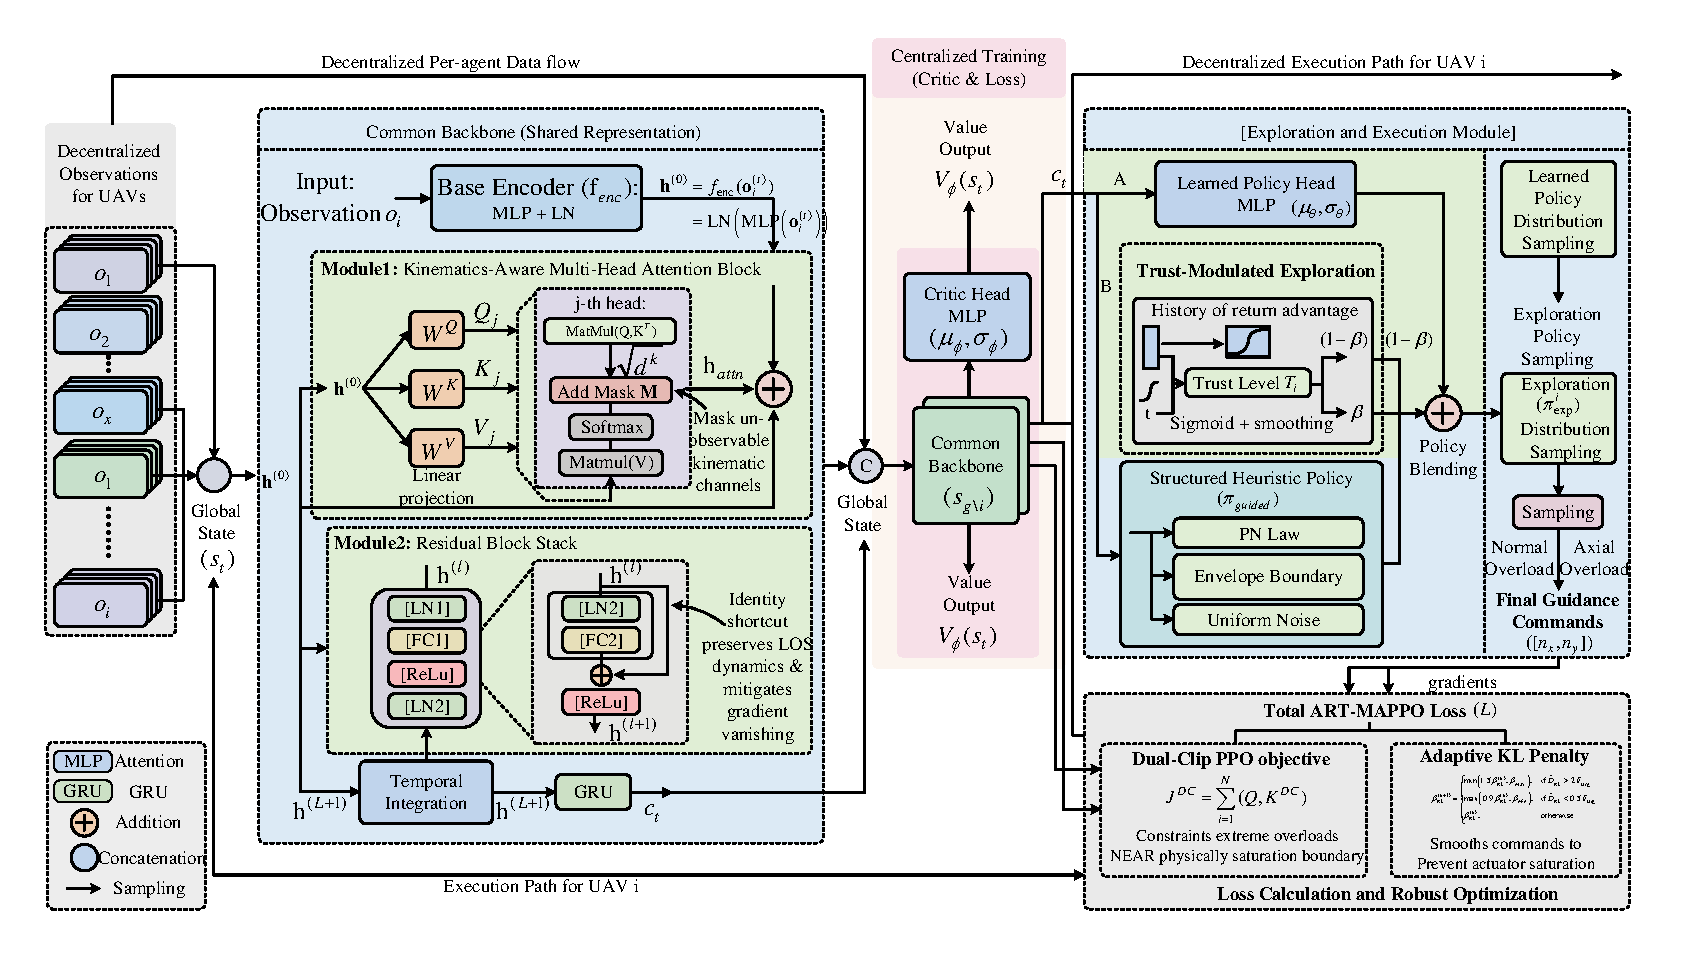
\includegraphics[width=7.3in]{rlsuanfa.pdf}
%DIFDELCMD < %%%
\DIFdelendFL \DIFaddbeginFL 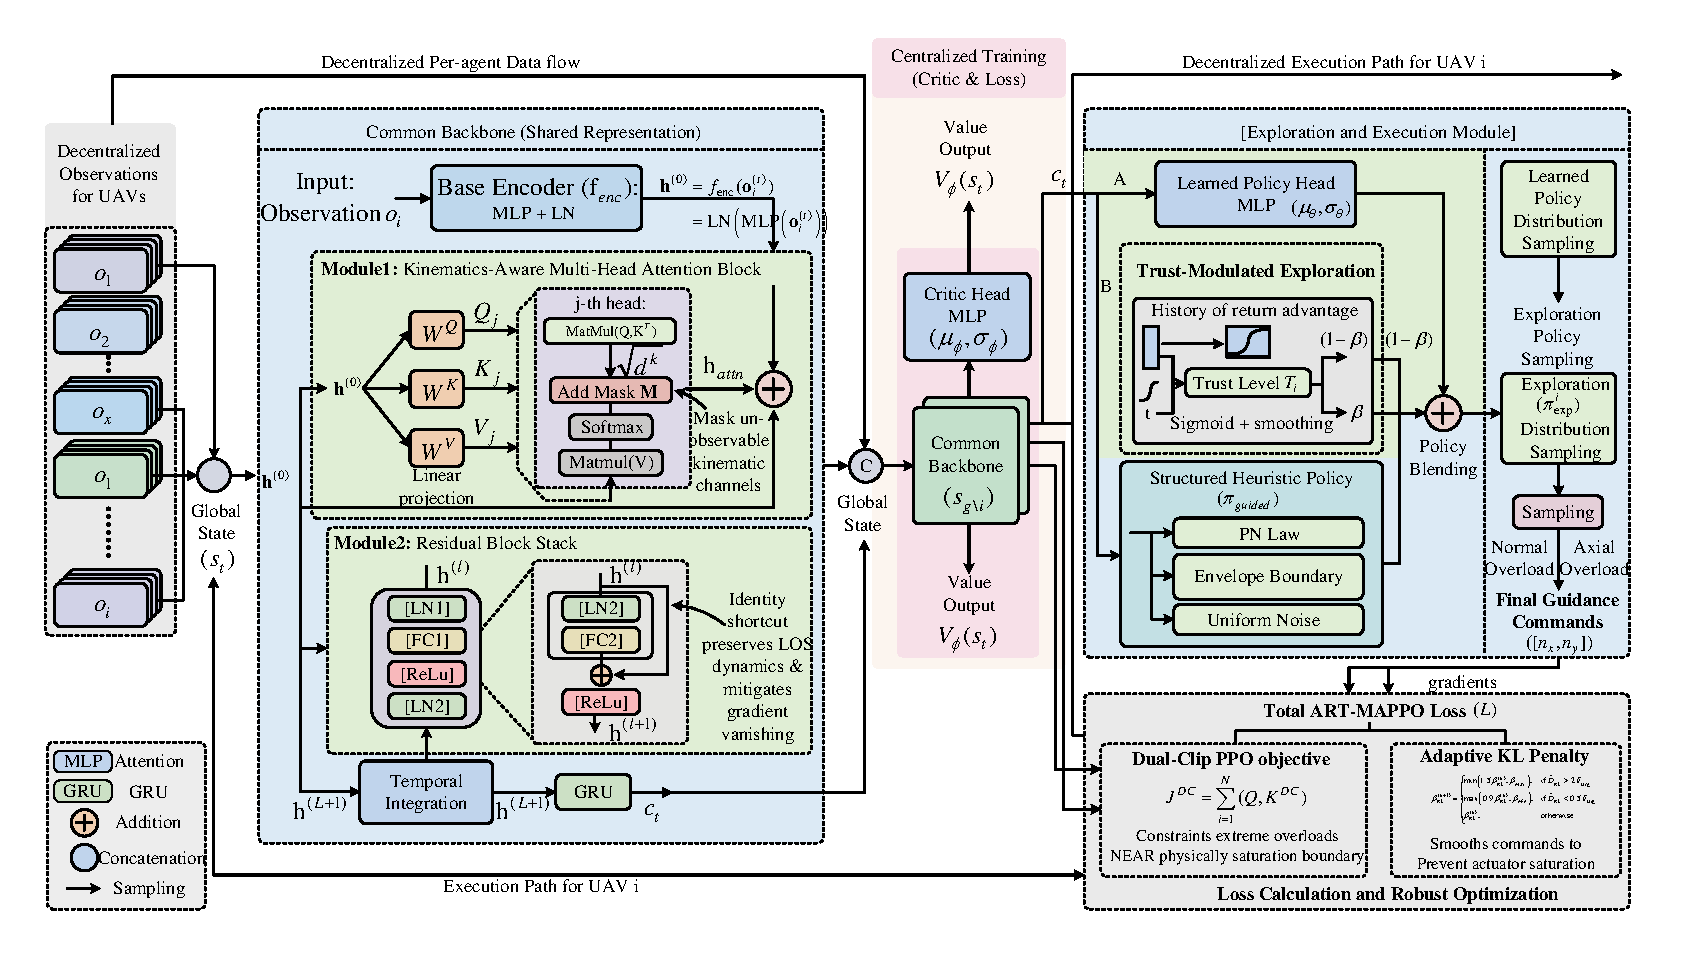
\includegraphics[width=7.0in]{rlsuanfa.pdf}
\DIFaddendFL \caption{\DIFdelbeginFL \DIFdelFL{Overall workflow of the }\DIFdelendFL ART-MAPPO \DIFdelbeginFL \DIFdelFL{algorithm for cooperative swarm interception, showing the interaction among the }\DIFdelendFL \DIFaddbeginFL \DIFaddFL{information flow from physical observations through }\DIFaddendFL attention-residual \DIFdelbeginFL \DIFdelFL{network, }\DIFdelendFL \DIFaddbeginFL \DIFaddFL{and
recurrent encoding to }\DIFaddendFL trust-modulated exploration \DIFdelbeginFL \DIFdelFL{, }\DIFdelendFL and \DIFdelbeginFL \DIFdelFL{dual-clip adaptive KL optimization}\DIFdelendFL \DIFaddbeginFL \DIFaddFL{regularized actor--critic updates}\DIFaddendFL .}
\label{fig:algorithm_flow}
\end{figure*}

\subsection{State Representation and Reward Design}
\label{subsec:state_reward}

\DIFdelbegin \emph{\DIFdel{1) Observation Space:}} %DIFAUXCMD
\DIFdel{The observation vector for interceptor $i$ at time step $t$ is designed to capture the essential kinematic quantities for guidance and
coordination:
}\begin{displaymath}
\DIFdel{
\mathbf{o}_i^{(t)} = \left[o_i^{(t),1},\; o_i^{(t),2},\; o_i^{(t),3},\; o_i^{(t),4}\right]^\top \in \mathbb{R}^{n_o},\quad n_o = 4
}\end{displaymath}%DIFAUXCMD
\DIFdel{The four components are defined as:
%DIF <  \begin{align}
%DIF <  o_i^{(t),1} &= \begin{cases} \dfrac{V_i \dot{q}_t}{g}, & |\dot{q}_t - \dot{q}_{t-1}| \leq \Delta\dot{q}_{\max} \\[6pt] \dfrac{V_i \dot{q}_{t-1}}{g}, & |\dot{q}_t - \dot{q}_{t-1}| > \Delta\dot{q}_{\max} \end{cases} \label{eq:o1} \\[6pt]
%DIF <  o_i^{(t),2} &= \gamma_{D_i} - q_i \label{eq:o2} \\[4pt]
%DIF <  o_i^{(t),3} &= \left(n_{x_i}^2 + n_{y_i}^2\right) \cdot \Delta t \label{eq:o3} \\[4pt]
%DIF <  o_i^{(t),4} &= \frac{r_i}{\min_{j \in \mathcal{G}_i} t_{go_j}} - V_i \label{eq:o4}
%DIF <  \end{align}
}\begin{align*}
\DIFdel{o_i^{(t),1} }&\DIFdel{=
\begin{cases}
\dfrac{V_i \dot{q}_i^{(t)}}{g}, &
\left|\dot{q}_i^{(t)} - \dot{q}_i^{(t-1)}\right| \leq \Delta \dot{q}_{\max}
\\[6pt]
\dfrac{V_i \dot{q}_i^{(t-1)}}{g}, &
\left|\dot{q}_i^{(t)} - \dot{q}_i^{(t-1)}\right| > \Delta \dot{q}_{\max}
\end{cases}
%
}\\[6pt]
\DIFdel{o_i^{(t),2} }&\DIFdel{= \gamma_{D_i} - q_i
%
}\\[4pt]
\DIFdel{o_i^{(t),3} }&\DIFdel{= \left(n_{x_i}^2 + n_{y_i}^2\right)\cdot \Delta t
%
}\\[4pt]
\DIFdel{o_i^{(t),4} }&\DIFdel{= \frac{r_i}{\min_{j \in \mathcal{G}_i} t_{go_j}} - V_i
%DIFDELCMD < \label{eq:o4}%%%
}\end{align*}%DIFAUXCMD
\DIFdelend \DIFaddbegin \DIFadd{The local observation retains relative three-dimensional geometry, cooperative timing, and
the previous applied command. Using fixed physical scales, it is
}\begin{equation}
\DIFadd{\label{eq:observation_space}
\begin{split}
\mathbf o_i^{(t)}=\operatorname{clip}\bigl([&
d_i/d_{\mathrm{ref}},\ \Delta z_i/z_{\mathrm{ref}},\
\dot d_i/V_{\mathrm{ref}},\ e_{\angle,i}/\pi,\\
&V_i/V_{\mathrm{ref}},\ V_{T(i)}/V_{\mathrm{ref}},\
\theta_i/\pi,\ \gamma_i/\pi,\ \boldsymbol\ell_{iT}^{\top},\\
&(t_{go,i}-\bar t_{go,i})/T_{\mathrm{ref}},\
(t_{go,i}^{\max}-t_{go,i}^{\min})/T_{\mathrm{ref}},\\
&(t_{go,i}-t_{go,i}^{\min})/T_{\mathrm{ref}},\
(\mathbf a_i^{(t-1)})^{\top}]^{\top},-1,1\bigr)
\in\mathbb R^{17}.
\end{split}
}\end{equation}\DIFaddend 
\DIFdelbegin \DIFdel{where $\Delta\dot{q}_{\max} = 0.03$~rad/s is the LOS-rate noise threshold,
$\mathcal{G}_i$ denotes the set of interceptors assigned to the same target as interceptor $i$, and
$\Delta t$ is the
simulation timestep. Component $o_i^{(t),1}$ is a smoothed required normal acceleration proportional to $V_i \dot{q}_i^{(t)} / g$,
where the previous LOS-rate estimate is retained when the
instantaneous measurement jump exceeds $\Delta \dot{q}_{\max}$. Component $o_i^{(t),2}$ }\DIFdelend \DIFaddbegin \DIFadd{Here, $\Delta z_i$ is the defender--target altitude difference,
$\boldsymbol\ell_{iT}\in\mathbb R^3$ }\DIFaddend is the \DIFdelbegin \DIFdel{lead-angle deviation driving heading correction, where $q_i$ (and its derivative $\dot{q}_i$) denotes the specific line-of-sight (LOS) angle between interceptor $i$ and its dynamically assigned target. 
Component $o_i^{(t),3}$ encodes the instantaneous control energy expenditure. Component $o_i^{(t),4}$ is }\DIFdelend \DIFaddbegin \DIFadd{LOS unit vector, and
$\widehat{\mathbf v}_i=\mathbf v_i/(\|\mathbf v_i\|_2+\varepsilon_{\mathrm{num}})$ is the
unit velocity direction. Therefore,
$e_{\angle,i}=\arccos[\operatorname{clip}(\widehat{\mathbf v}_i^{\top}
\boldsymbol\ell_{iT},-1,1)]$ is }\DIFaddend the
\DIFdelbegin \DIFdel{velocity error relative to the desired approach speed $r_i / \min_j t_{go_j}$, which drives time-coordinated impact.
}%DIFDELCMD < 

%DIFDELCMD < %%%
\emph{\DIFdel{2) Reward Function:}} %DIFAUXCMD
\DIFdel{The reward function incorporates five components to guide the learning process:
}\begin{displaymath}
\DIFdel{
\begin{split}
r_i^{(t)} =& \; w_1 r_i^{\text{dist}} + w_2 r_i^{\text{angle}} + w_3 r_i^{\text{hit}} \\
&+ w_4 r_i^{\text{coord}} + w_5 r_i^{\text{energy}}
\end{split}
}\end{displaymath}%DIFAUXCMD
\DIFdel{with each component defined as:
}\begin{align*}
\DIFdel{r_i^{\text{dist}} }&\DIFdel{= \exp\!\left(-\alpha_d \left\|\mathbf{p}_i^{(t)} - \mathbf{p}_{\text{tgt}}\right\|\right) }\\
\DIFdel{r_i^{\text{angle}} }&\DIFdel{= -\alpha_a \left|\gamma_{D_i} - q_i\right| }\\
\DIFdel{r_i^{\text{hit}} }&\DIFdel{= R_{\text{hit}} \cdot \mathbb{I}\!\left(\left\|\mathbf{p}_i^{(t)} - \mathbf{p}_{\text{tgt}}\right\| < d_{\text{kill}}\right) }\\
\DIFdel{r_i^{\text{coord}} }&\DIFdel{= -\alpha_c \left| t_{go_i}^{(t)} - \bar{t}_{go}^{(t)} \right|, \quad \bar{t}_{go}^{(t)} = \frac{1}{|\mathcal{G}_i|}\sum_{j \in \mathcal{G}_i} t_{go_j}^{(t)} }\\
\DIFdel{r_i^{\text{energy}} }&\DIFdel{= -\alpha_e \left(n_{x_i}^2 + n_{y_i}^2\right) 
}\end{align*}%DIFAUXCMD
\DIFdel{where $\mathbf{p}_i^{(t)} = [x_i, y_i]^\top$ is the interceptor position, $\mathbf{p}_{\text{tgt}}$ is the target position, $d_{\text{kill}}$ is the lethal radius, $R_{\text{hit}} > 0$ is the terminal success reward, and $w_k$, $\alpha_k$ are weighting coefficients.
The distance reward $r_i^{\text{dist}} \in (0,1]$ provides dense, bounded feedback for target approach.The coordination reward $r_i^{\text{coord}}$ penalizes deviation from the group mean }\DIFdelend \DIFaddbegin \DIFadd{three-dimensional velocity-to-LOS angle. The mean, minimum, and maximum }\DIFaddend time-to-go \DIFdelbegin \DIFdel{$\bar{t}_{go}^{(t)}$, encouraging simultaneous impact;
this term is computed by the centralized critic during training and obtained via inter-agent communication during execution.The energy term $r_i^{\text{energy}}$ regularizes control effort to prevent actuator saturation.}%DIFDELCMD < 

%DIFDELCMD < %%%
\subsection{\DIFdel{Evaluation Criteria}}
%DIFAUXCMD
\addtocounter{subsection}{-1}%DIFAUXCMD
%DIFDELCMD < \label{subsec:eval}
%DIFDELCMD < %%%
\DIFdelend \DIFaddbegin \DIFadd{values are
computed over the cooperative group $\mathcal G_i$. The previous command is available before
the current action is selected and supplies short-term actuator history without violating
causality. Fixed scales $d_{\mathrm{ref}},z_{\mathrm{ref}},V_{\mathrm{ref}}$, and
$T_{\mathrm{ref}}$ make the heterogeneous physical channels comparable.
}\DIFaddend 

\DIFdelbegin \DIFdel{To quantitatively evaluate the proposed cooperative interception method, we adopt four metrics that capture temporal coordination, terminal load safety, guidance accuracy, and operational efficiency.}\DIFdelend The \DIFdelbegin \DIFdel{first three metrics are formally defined as follows.
}\begin{displaymath}
\DIFdel{%DIFDELCMD < \label{E1}%%%
E_{co\text{-}time} = \frac{1}{m}\sum_{i=1}^{m} \left| t_{go_i} - \frac{1}{m}\sum_{j=1}^{m} t_{go_j} \right|
}\end{displaymath}%DIFAUXCMD
\begin{displaymath}
\DIFdel{%DIFDELCMD < \label{E2}%%%
E_{n} = \frac{1}{m}\sum_{i=1}^{m} |n_{y_i}|
}\end{displaymath}%DIFAUXCMD
\begin{displaymath}
\DIFdel{%DIFDELCMD < \label{E3}%%%
E_{miss} = \frac{1}{m}\sum_{i=1}^{m} d_{tf_i}
}\end{displaymath}%DIFAUXCMD
\DIFdelend \DIFaddbegin \DIFadd{reward connects each physical objective to one interpretable component:
}\begin{equation}
\DIFadd{\label{eq:reward_function}
r_i^{(t)}=\lambda_d r_i^{\mathrm{dist}}
+\lambda_q r_i^{\mathrm{angle}}
+\lambda_h r_i^{\mathrm{hit}}
+\lambda_c r_i^{\mathrm{coord}}
+\lambda_u r_i^{\mathrm{effort}}.
}\end{equation}\DIFaddend 
\DIFaddbegin \DIFadd{The components are summarized below to avoid another rapid sequence of five displayed
equations.
}\begin{table}[!t]
\centering
\caption{\DIFaddFL{Reward Components and Physical Roles}}
\label{tab:reward_components}
\renewcommand{\arraystretch}{1.15}
\footnotesize
\begin{tabular}{@{}p{0.25\linewidth}p{0.67\linewidth}@{}}
\toprule
\DIFaddFL{Component }& \DIFaddFL{Definition and role }\\
\midrule
\DIFaddFL{$r_i^{\mathrm{dist}}$
}& \DIFaddFL{$\exp[-\|\mathbf p_i-\mathbf p_{\mathrm{tgt}}\|/d_{\mathrm{ref}}]$;
bounded dense feedback for closing range.}\\
\DIFaddFL{$r_i^{\mathrm{angle}}$
}& \DIFaddFL{$-e_{\angle,i}$; penalizes three-dimensional velocity-to-LOS misalignment.}\\
\DIFaddFL{$r_i^{\mathrm{hit}}$
}& \DIFaddFL{$R_{\mathrm{hit}}\mathbb I[\text{first entry into }d_{\mathrm{kill}}]$;
one-time terminal success reward.}\\
\DIFaddFL{$r_i^{\mathrm{coord}}$
}& \DIFaddFL{$-|t_{go,i}-|\mathcal G_i|^{-1}\sum_{j\in\mathcal G_i}t_{go,j}|$;
promotes simultaneous arrival.}\\
\DIFaddFL{$r_i^{\mathrm{effort}}$
}& \DIFaddFL{$-[\|\mathbf a_i^{(t)}\|_2^2+\kappa_{\Delta}
\|\mathbf a_i^{(t)}-\mathbf a_i^{(t-1)}\|_2^2]$;
penalizes all three load channels and their command variation.}\\
\bottomrule
\end{tabular}
\end{table}
\DIFadd{The environment computes these rewards during training; the critic estimates their discounted
return but does not generate the reward. At deployment, no reward or centralized critic is
required.
}\DIFaddend 

\DIFdelbegin \DIFdel{Here, Eq.~}%DIFDELCMD < \eqref{E1} %%%
\DIFdel{measures the mean deviation of individual time-to-go values from the group mean, thereby assessing temporal coordination among interceptors assigned to the same target. Eq.
~}%DIFDELCMD < \eqref{E2} %%%
\DIFdel{gives the average terminal normal overload, which reflects control effort and maneuver aggressiveness during the terminal guidance phase. Eq. ~}%DIFDELCMD < \eqref{E3} %%%
\DIFdel{denotes the mean terminal miss distance, where $d_{tf_i}$ is the relative distance between interceptor $i$ and its assigned target at the terminal engagement time $t_{f_i}$, serving as a direct indicator of guidance accuracy.
The fourth metric, coordinated interception duration, quantifies operational efficiency and is reported as the mean elapsed time between the earliest and latest terminal engagements within each coordinated group. All four metrics are reported in }\DIFdelend \DIFaddbegin \subsection{\DIFadd{Sensitivity of Reward Weights and Hyperparameters}}
\label{subsec:reward_sensitivity}

\DIFadd{The weights $\lambda_d$ and $\lambda_q$ regulate early approach and heading alignment, whereas
$\lambda_h$ and $\lambda_c$ determine the balance between terminal interception and coordinated
arrival. Excessive coordination weight can delay a defender with favorable geometry; excessive
effort weight $\lambda_u$ can suppress the normal-load commands required against a maneuvering
target. We therefore normalize all reward components first, tune hit/coordination weights around
mission success, and then increase the effort term until command peaks and variations satisfy
the desired envelope without degrading interception reliability.
}

\DIFadd{The PPO clipping factor $\varepsilon_{\mathrm{PPO}}$, dual-clip parameter $c_{\mathrm{DC}}$,
target divergence $\delta_{\mathrm{KL}}$, and $\beta_{\mathrm{KL}}$ adaptation determine policy
update conservatism. Smaller clipping/divergence targets improve stability but can slow
adaptation; larger values learn aggressive maneuvers faster but increase return variance.
$\lambda_{\mathrm{GAE}}$ and $c_e$ control the bias--variance and exploration--exploitation
tradeoffs. Their numerical settings and sensitivity tests are reported with }\DIFaddend the simulation
results \DIFdelbegin \DIFdel{to provide a comprehensive assessment of effectiveness, safety, precision, and efficiency.
}\DIFdelend \DIFaddbegin \DIFadd{rather than expanded into additional equations here.
}

\begin{algorithm}[!t]
\caption{\DIFadd{ART-MAPPO Cooperative Interception Guidance}}
\label{alg:artmappo}
\footnotesize
\begin{algorithmic}[1]
\REQUIRE \DIFadd{Consensus assignment $\mathbf X^{*}$, environment, episode horizon
$H_{\mathrm{ep}}$, actor $\theta$, critic $\phi$, trust and PPO parameters
}\ENSURE \DIFadd{Decentralized shared guidance policy $\pi_{\theta}$
}\STATE \DIFadd{Initialize networks, GRU states $\mathbf g_i$, trust states $\mathcal T_i$, and buffer
$\mathcal D$
}\FOR{episode $k=1,2,\ldots$}
    \STATE \DIFadd{Reset the scenario and form cooperative groups from $\mathbf X^{*}$
    }\FOR{$t=0$ to $H_{\mathrm{ep}}-1$}
        \FOR{each defender $i$}
            \STATE \DIFadd{Construct $\mathbf o_i^{(t)}$ using }\eqref{eq:observation_space}
            \STATE \DIFadd{Encode attention/residual features and update $\mathbf g_i^{(t)}$
            }\STATE \DIFadd{Sample $\mathbf a_i^{(t)}$ from }\eqref{eq:exploration_policy} \DIFadd{and clip it
            to $\mathcal A$
        }\ENDFOR
        \STATE \DIFadd{Execute the joint action and compute }\eqref{eq:reward_function}
        \STATE \DIFadd{Store the transition in $\mathcal D$
    }\ENDFOR
    \STATE \DIFadd{Update return statistics and trust using
    }\eqref{eq:trust_statistics}\DIFadd{--}\eqref{eq:trust_update}
    \STATE \DIFadd{Estimate $\widehat A_t$ using }\eqref{eq:gae}
    \STATE \DIFadd{Update actor and critic by minimizing }\eqref{eq:total_loss}\DIFadd{; adapt
    $\beta_{\mathrm{KL}}$ using }\eqref{eq:kl_adaptation}
    \STATE \DIFadd{Clear $\mathcal D$
}\ENDFOR
\STATE \DIFadd{Deploy $\pi_{\theta}$ with local observations, local GRU states, and $\beta_i=0$
}\end{algorithmic}
\end{algorithm}
 \DIFaddend 

%DIF < % ===========================================================
\section{Simulation Verification}
\label{sec:simulation}

\subsection{Experimental Setup and Implementation Details}
\label{subsec:setup}

All training and evaluation were performed on an Intel Core i7-9700F CPU / Nvidia RTX 3090
GPU server running Ubuntu 18.04.
The simulation step size was 0.05\,s \DIFaddbegin \DIFadd{and the maximum episode duration was 75\,s}\DIFaddend .
Table~\ref{table2} summarizes the key hyperparameters of ART-MAPPO.

\begin{table}[!t]
\centering
\renewcommand{\arraystretch}{1.4}
\caption{ART-MAPPO Algorithm Parameters}
\label{table2}
\begin{tabular}{ll}
\hline\hline
Parameter & Value \\ \hline
PPO clipping factor (\DIFdelbeginFL \DIFdelFL{$\epsilon$}\DIFdelendFL \DIFaddbeginFL \DIFaddFL{$\varepsilon_{\mathrm{PPO}}$}\DIFaddendFL ) & 0.2 \\
Dual-clip parameter (\DIFdelbeginFL \DIFdelFL{$c$}\DIFdelendFL \DIFaddbeginFL \DIFaddFL{$c_{\mathrm{DC}}$}\DIFaddendFL ) & 3.0 \\
Target KL divergence (\DIFdelbeginFL \DIFdelFL{$\delta_{\text{targ}}$}\DIFdelendFL \DIFaddbeginFL \DIFaddFL{$\delta_{\mathrm{KL}}$}\DIFaddendFL ) & 0.02 \\
Entropy bonus coefficient ($c_e$) & 0.01 \\
GAE parameter ($\lambda_{\mathrm{GAE}}$) & 0.97 \\
LR schedule & Cosine Annealing \\
Optimizer & AdamW \\
Mini-batch number & 4 \\
Buffer size & 4096 \\
Learning rate & $3\times10^{-4}$ \\
Attention heads ($H$) & 4 \\
Residual blocks ($L$) & 2 \\ \hline
\end{tabular}
\end{table}


The \DIFaddbegin \DIFadd{horizontal projection of the }\DIFaddend simulation environment is depicted in Fig.~\ref{chushi}.
\DIFdelbegin \DIFdel{$A_{\text{UAV}}$ are randomly spawned within an annular region of radii $D_1$--$D_2$}\DIFdelend \DIFaddbegin \DIFadd{In the three-dimensional case presets, the 20 defenders start near the defended center at
radii 52.63--65.44}\DIFaddend \,m \DIFdelbegin \DIFdel{with speed
$V_A\in[10,40]$}\DIFdelend \DIFaddbegin \DIFadd{and altitude 0}\DIFaddend \,m\DIFdelbegin \DIFdel{/s. To simulate a directional swarm attack toward the high-value target area, their initial heading angles $\gamma_A$ are uniformly distributed within $[q_A-30^\circ, q_A+30^\circ]$, where $q_A$ explicitly denotes the initial line-of-sight (LOS) angle from the specific attacker to the center of the defended area. $D_{\text{UAV}}$ are
uniformly distributed within a disk of radius $D_3$}\DIFdelend \DIFaddbegin \DIFadd{, while the eight attackers start at radii
1987.72--2145.95\,m and altitude 120\,m. Initial defender and attacker speeds are
20.32--30.02}\DIFaddend \,m\DIFdelbegin \DIFdel{with
$V_D\in[10,40]$}\DIFdelend \DIFaddbegin \DIFadd{/s and 30.23--45.87}\DIFaddend \,m/s\DIFdelbegin \DIFdel{and $\gamma_D\in[0,2\pi]$}\DIFdelend \DIFaddbegin \DIFadd{, respectively. The attackers initially point toward
the defended region and then execute the case-specific three-dimensional maneuvers described
below}\DIFaddend .


\begin{figure}[!t]
\centering
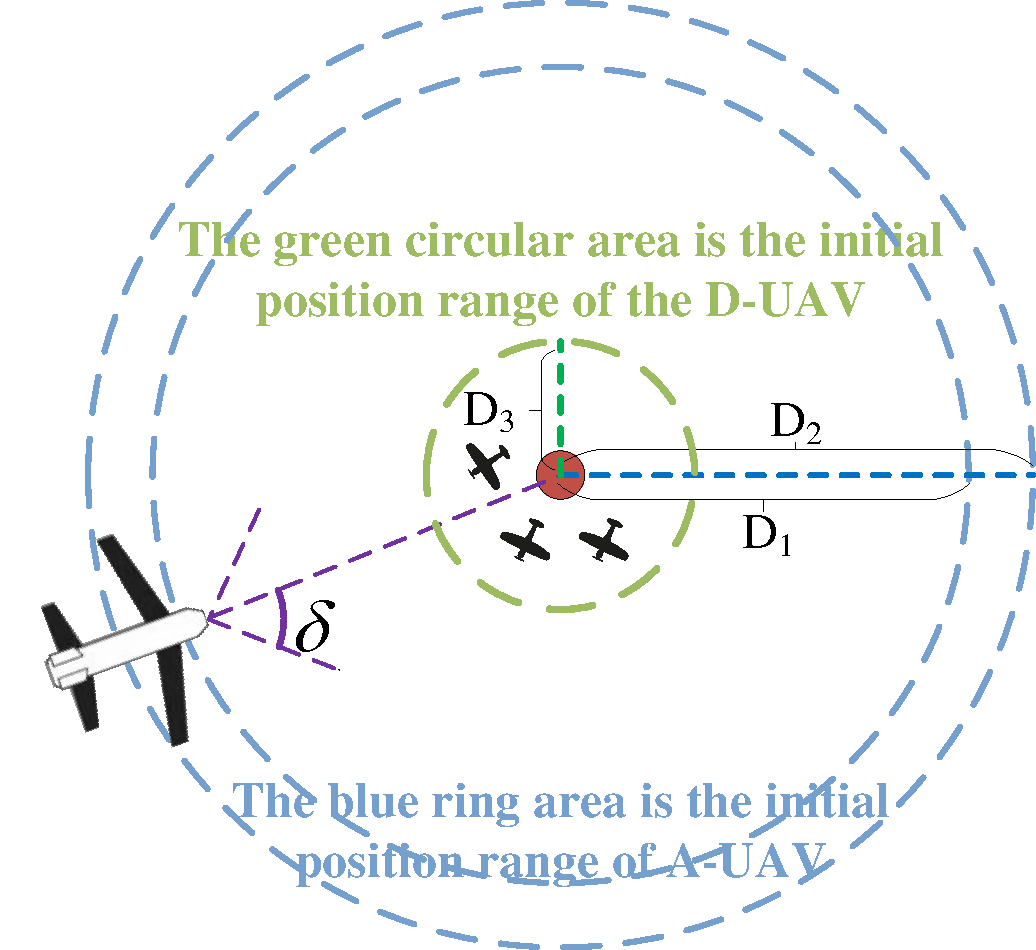
\includegraphics[width=3.0in]{chushi01.pdf}
\caption{Simulation environment configuration for training.}
\label{chushi}
\end{figure}

A representative scenario of 20 $D_{\text{UAV}}$ versus 8 $A_{\text{UAV}}$ is considered\DIFdelbegin \DIFdel{, with $D_1=100$\,m,
$D_2=1500$\,m, and $D_3=1600$\,m}\DIFdelend .
Table~\ref{chushicanshu} summarizes the \DIFdelbegin \DIFdel{UAV kinematic parameters}\DIFdelend \DIFaddbegin \DIFadd{audited three-dimensional initialization and
kinematic constraints}\DIFaddend .

\begin{table*}[!t]
\centering
\caption{UAV Parameters for Attackers and Defenders}
\label{chushicanshu}
\renewcommand{\arraystretch}{1.6}
\begin{tabular}{ccccc}
\hline\hline
 & Initial \DIFdelbeginFL \DIFdelFL{position $(x,y)$ }\DIFdelendFL \DIFaddbeginFL \DIFaddFL{radius / altitude }\DIFaddendFL & Initial velocity $V$ & Initial heading $\gamma$ & Maneuverability \DIFdelbeginFL \DIFdelFL{$(n_x,n_y,V)$ }\DIFdelendFL \DIFaddbeginFL \DIFaddFL{$(n_x,n_y,n_z)$ }\DIFaddendFL \\ \hline
$D_{\text{UAV}}$ & \DIFdelbeginFL \DIFdelFL{$r\sim U[0,D_3]$, $\theta\sim U[0,2\pi]$ }\DIFdelendFL \DIFaddbeginFL \DIFaddFL{52.63--65.44\,m / 0\,m }\DIFaddendFL & \DIFdelbeginFL \DIFdelFL{$V_D\sim U[10,40]$}\DIFdelendFL \DIFaddbeginFL \DIFaddFL{20.32--30.02}\DIFaddendFL \,m/s & \DIFdelbeginFL \DIFdelFL{$\gamma_D\sim U[0,2\pi]$ }\DIFdelendFL \DIFaddbeginFL \DIFaddFL{$\gamma_D\in[0,2\pi]$ }\DIFaddendFL & \DIFdelbeginFL \DIFdelFL{$n_x\in[-0.1g,1g]$, $n_y\in[-1g,1g]$ }\DIFdelendFL \DIFaddbeginFL \DIFaddFL{$n_x\in[-0.1,1]$, $n_y,n_z\in[-1,1]$ }\DIFaddendFL \\
$A_{\text{UAV}}$ & \DIFdelbeginFL \DIFdelFL{$r\sim U[D_1,D_2]$, $\theta\sim U[0,2\pi]$ }\DIFdelendFL \DIFaddbeginFL \DIFaddFL{1987.72--2145.95\,m / 120\,m }\DIFaddendFL & \DIFdelbeginFL \DIFdelFL{$V_A\sim U[10,40]$}\DIFdelendFL \DIFaddbeginFL \DIFaddFL{30.23--45.87}\DIFaddendFL \,m/s & \DIFdelbeginFL \DIFdelFL{$\gamma_A\sim U[q_A-30^\circ,q_A+30^\circ]$ }\DIFdelendFL \DIFaddbeginFL \DIFaddFL{Toward defended area }\DIFaddendFL & \DIFdelbeginFL \DIFdelFL{$n_x=0$, $n_y\in[-1g,1g]$ }\DIFdelendFL \DIFaddbeginFL \DIFaddFL{Case-specific 3-D maneuver }\DIFaddendFL \\ \hline
\end{tabular}
\end{table*}

Two dynamic engagement scenarios are designed to evaluate cooperative guidance performance.
The scenario configurations are listed in Table~\ref{changjingqingkuang}.

\begin{table}[!t]
\centering
\renewcommand{\arraystretch}{1.4}
\caption{Combat Scenario Settings}
\label{changjingqingkuang}
\begin{tabular}{cccc}
\hline\hline
 & $N_{D\text{-UAV}}$ & $N_{A\text{-UAV}}$ & $A_{\text{UAV}}$ Strategy \\ \hline
Case 1 & 20 & 8 & Hybrid Evasion \\
Case 2 & 20 & 8 & Sinusoidal Maneuver \\ \hline
\end{tabular}
\end{table}

\DIFaddbegin \DIFadd{To represent delayed communication and sensing uncertainty, every defender receives the
position and velocity packets used to construct Eq.~}\eqref{eq:observation_space} \DIFadd{after an
end-to-end delay of 50\,ms. For each Cartesian component,
$\widehat{\mathbf p}(t)=\mathbf p(t-50\,\mathrm{ms})+\boldsymbol\eta_p$ with
$\boldsymbol\eta_p\sim\mathcal N(\mathbf0\,\mathrm{m},9\mathbf I_3\,\mathrm{m}^2)$, and
$\widehat{\mathbf v}(t)=\mathbf v(t-50\,\mathrm{ms})+\boldsymbol\eta_v$ with
$\boldsymbol\eta_v\sim\mathcal N(\mathbf0\,\mathrm{m/s},
0.09\mathbf I_3\,\mathrm{m}^2/\mathrm{s}^2)$. Thus, every position component has mean error
0\,m and variance 9\,m$^2$, while every velocity component has mean error 0\,m/s and variance
0.09\,(m/s)$^2$. Range, altitude difference, LOS direction, closing speed, heading, pitch,
velocity-to-LOS angle, and time-to-go are recomputed from these delayed noisy Cartesian states;
no additional independent noise is imposed on those derived quantities. Previous applied loads
are internally measured without additive observation noise, while the commanded loads pass
through a first-order response with a 300-ms time constant. Table~\ref{tab:uncertainty_settings}
summarizes these settings in physical units.
}

\begin{table}[!t]
\centering
\caption{\DIFaddFL{Communication Delay and Observation-Uncertainty Settings}}
\label{tab:uncertainty_settings}
\renewcommand{\arraystretch}{1.15}
\footnotesize
\begin{tabular}{@{}p{0.29\linewidth}p{0.20\linewidth}p{0.39\linewidth}@{}}
\toprule
\DIFaddFL{Observed quantity }& \DIFaddFL{Delay / response }& \DIFaddFL{Error distribution }\\
\midrule
\DIFaddFL{Position $x,y,z$ }& \DIFaddFL{50\,ms }& \DIFaddFL{Mean $0$\,m; variance $9$\,m$^2$ }\\
\DIFaddFL{Velocity $v_x,v_y,v_z$ }& \DIFaddFL{50\,ms }& \DIFaddFL{Mean $0$\,m/s; variance $0.09$\,(m/s)$^2$ }\\
\DIFaddFL{Derived geometry and $t_{go}$ }& \DIFaddFL{50\,ms }& \DIFaddFL{No independent noise; computed from $\widehat{\mathbf p},\widehat{\mathbf v}$ }\\
\DIFaddFL{Previous loads $n_x,n_y,n_z$ }& \DIFaddFL{300\,ms response }& \DIFaddFL{Mean $0$; variance $0$ }\\
\bottomrule
\end{tabular}
\end{table}




\subsection{\DIFadd{Evaluation Criteria}}
\label{subsec:eval}

\DIFadd{The evaluation metrics are defined from quantities measured at interception, rather than from
time-to-go values that vanish at the terminal instant. For target $t_j$, let
$\mathcal G_j=\{i:X_{ij}=1\}$ be its cooperative defender group,
$m_j=|\mathcal G_j|$, $t_i^{\mathrm{arr}}$ the first time defender $i$ reaches the lethal
radius, and $\mathcal W_i=[t_i^{\mathrm{arr}}-\Delta T_{\mathrm{term}},
t_i^{\mathrm{arr}}]$ the terminal measurement window. The four group-level metrics are
collected in one equation:
}\begin{equation}
\DIFadd{\label{eq:evaluation_metrics}
\begin{aligned}
\bar t_j^{\mathrm{arr}}
 &=\frac{1}{m_j}\sum_{i\in\mathcal G_j}t_i^{\mathrm{arr}},\\
E_{\mathrm{co\text{-}time}}^{(j)}
 &=\frac{1}{m_j}\sum_{i\in\mathcal G_j}
 \left|t_i^{\mathrm{arr}}-\bar t_j^{\mathrm{arr}}\right|,\\
\bar n_{i,\mathrm{term}}
 &=\frac{1}{|\mathcal W_i|}\sum_{t\in\mathcal W_i}
 \sqrt{(n_{y_i}^{(t)})^2+(n_{z_i}^{(t)})^2},\\
E_n^{(j)}
 &=\frac{1}{m_j}\sum_{i\in\mathcal G_j}
 \bar n_{i,\mathrm{term}},\\
E_{\mathrm{miss}}^{(j)}
 &=\frac{1}{m_j}\sum_{i\in\mathcal G_j}d_i(t_i^{\mathrm{arr}}),\\
E_t^{(j)}&=\max_{i\in\mathcal G_j}t_i^{\mathrm{arr}}-t_0.
\end{aligned}
}\end{equation}
\DIFadd{Here, $E_{\mathrm{co\text{-}time}}$ measures arrival-time dispersion,
$E_n$ is the mean terminal-window resultant normal load factor, $E_{\mathrm{miss}}$ is the terminal miss
distance, and $E_t$ is the time from engagement start $t_0$ until the last member of the group
arrives. This separates synchronization quality from total engagement duration. A trial-level
value is the mean of the corresponding group values over the eight targets. Monte Carlo
boxplots use successful trials only; interception success rate is reported separately so that
failed trials are not hidden by the conditional metric distributions.
 }

\DIFaddend \subsection{Target Assignment Performance and Spatial Topology}
\label{subsec:assignment_results}

To evaluate the IDBO algorithm, it is benchmarked against PSO, GWO, SSA, BOA, and standard DBO. 

Fig.~\ref{fig:convergence} illustrates the statistical performance in terms of average cost convergence over iterations. IDBO significantly outperforms the baselines, reaching the lowest steady-state cost within 100~iterations. \begin{figure}[!ht] 
\centering 
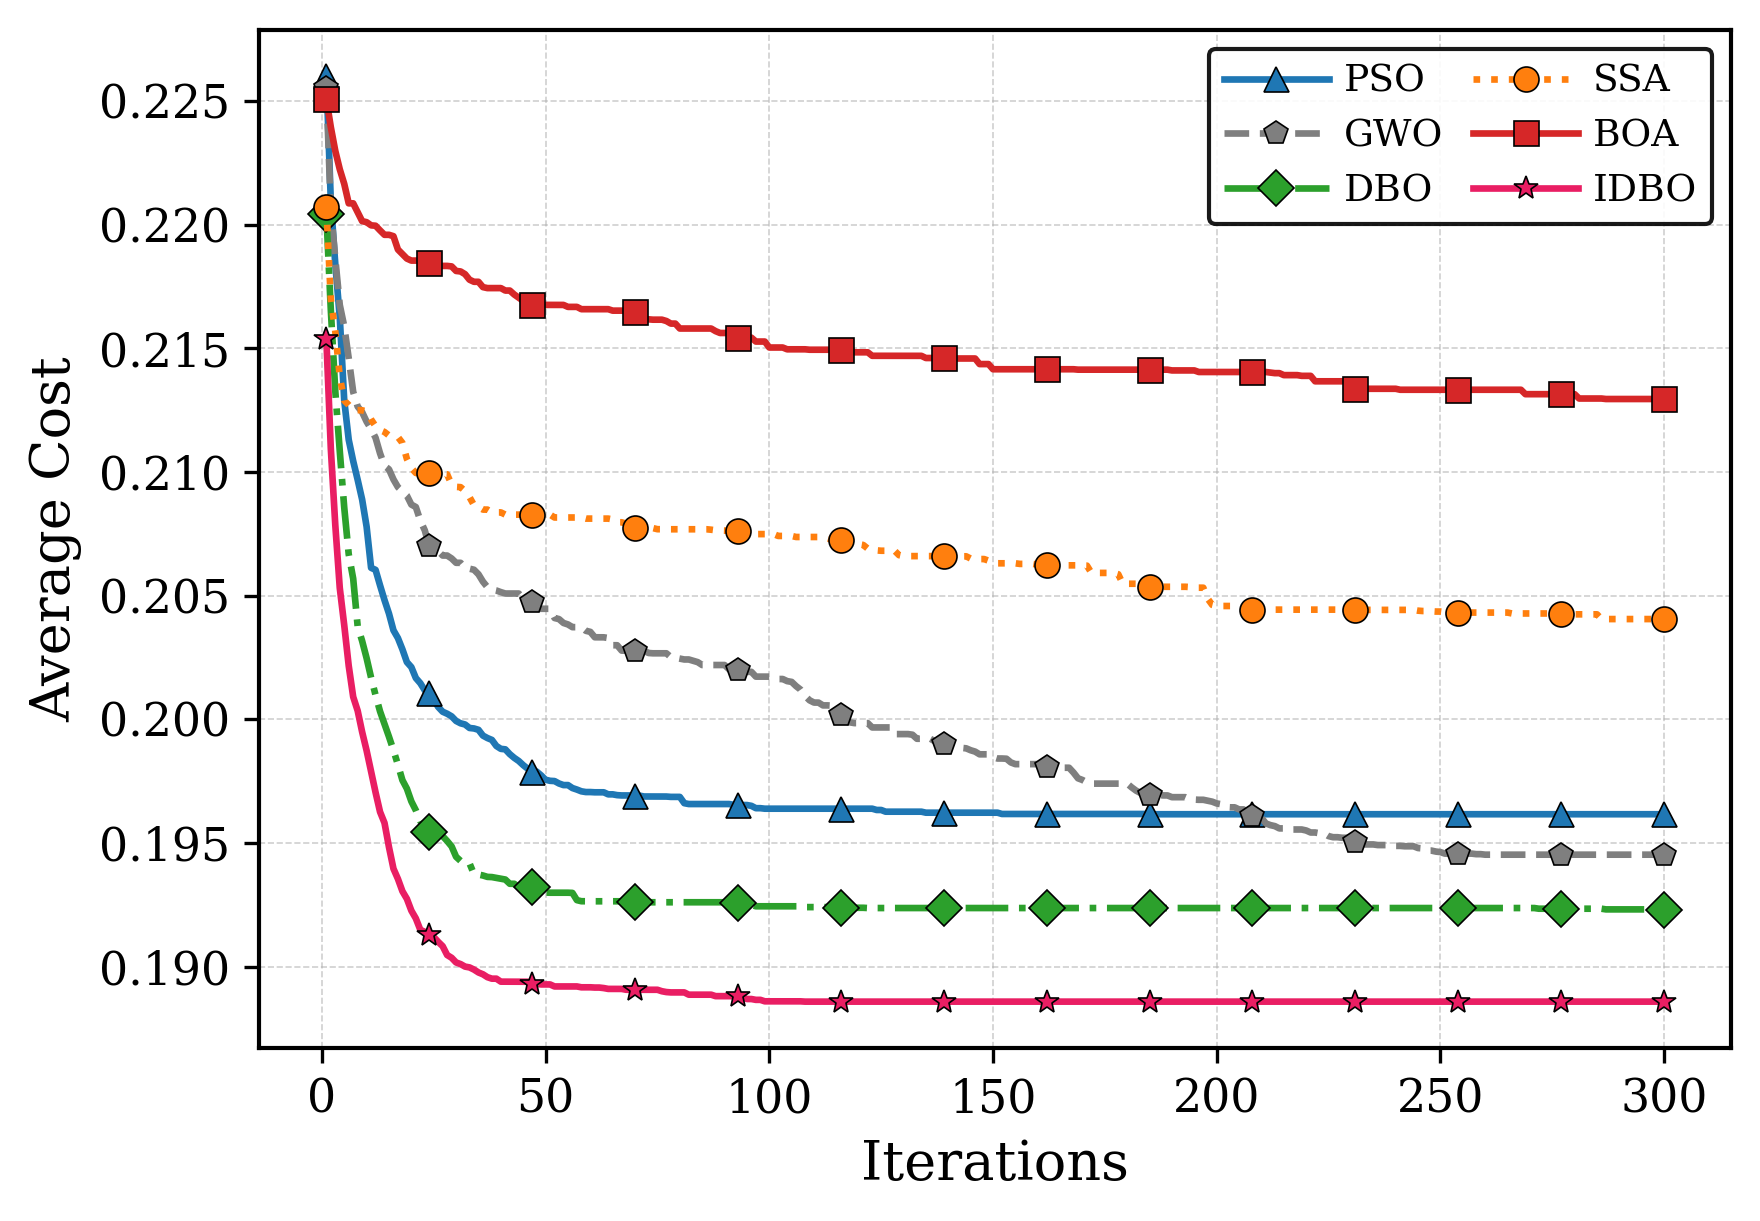
\includegraphics[width=3.25in]{convergence.png} 
\caption{Average cost convergence over iterations for target assignment algorithms.} 
\label{fig:convergence} 
\end{figure}

Furthermore, the violin plot in Fig.~\ref{fig:violin} evaluates the algorithmic robustness across multiple independent runs. It shows IDBO's compact distribution at the lowest median cost, highlighting its superior stability and consistency compared to the other heuristic methods.

\begin{figure}[!ht] 
\centering 
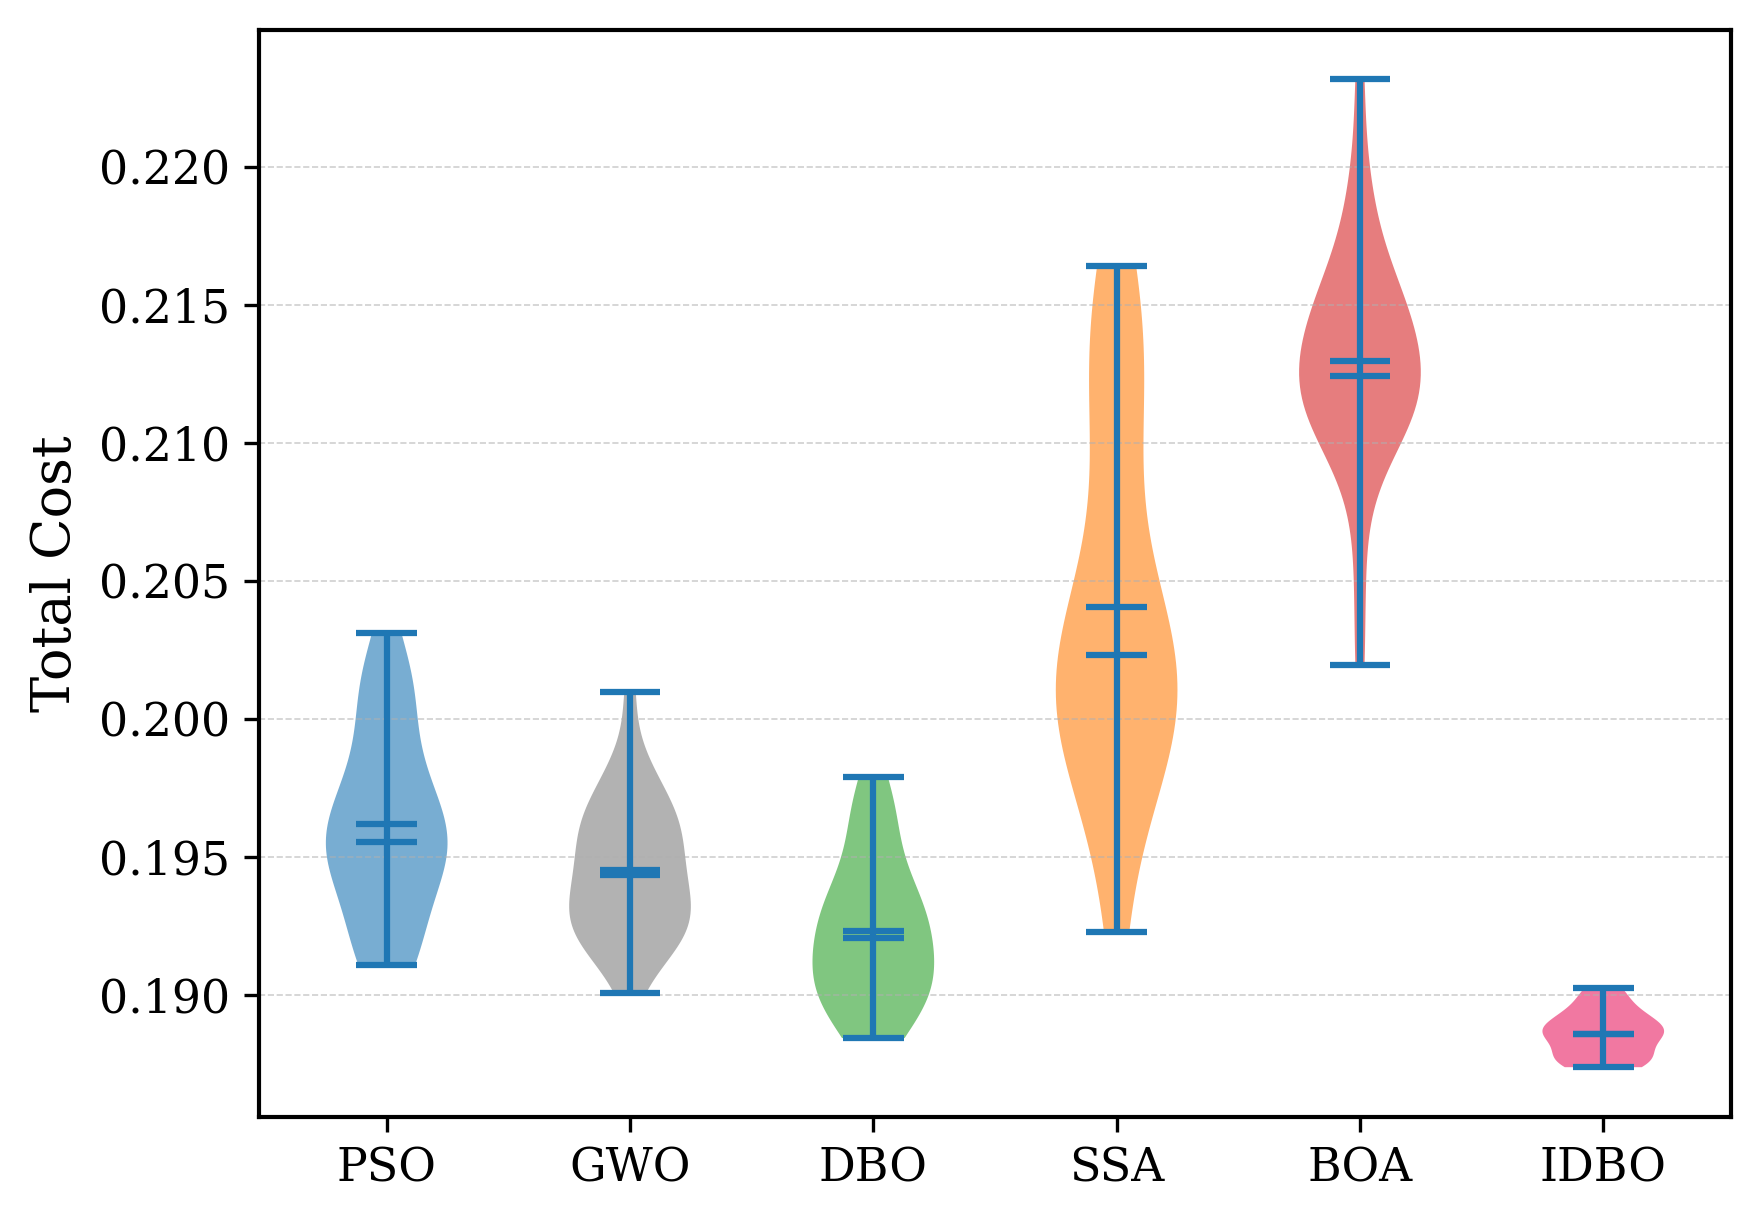
\includegraphics[width=3.2in]{violin.png} 
\caption{Violin plot of total cost distribution evaluating algorithm robustness.} 
\label{fig:violin} 
\end{figure}

The optimal assignment mapping generated by the algorithm is visualized in Fig.~\ref{fig:assignment_topology}. Attackers $A_1$--$A_4$ are each allocated three defenders, while $A_5$--$A_8$ are intercepted by two defenders each, perfectly respecting the per-target capacity constraint $L_{\max}$ and ensuring sufficient numerical superiority for cooperative strikes.

\begin{figure}[!ht]
\centering
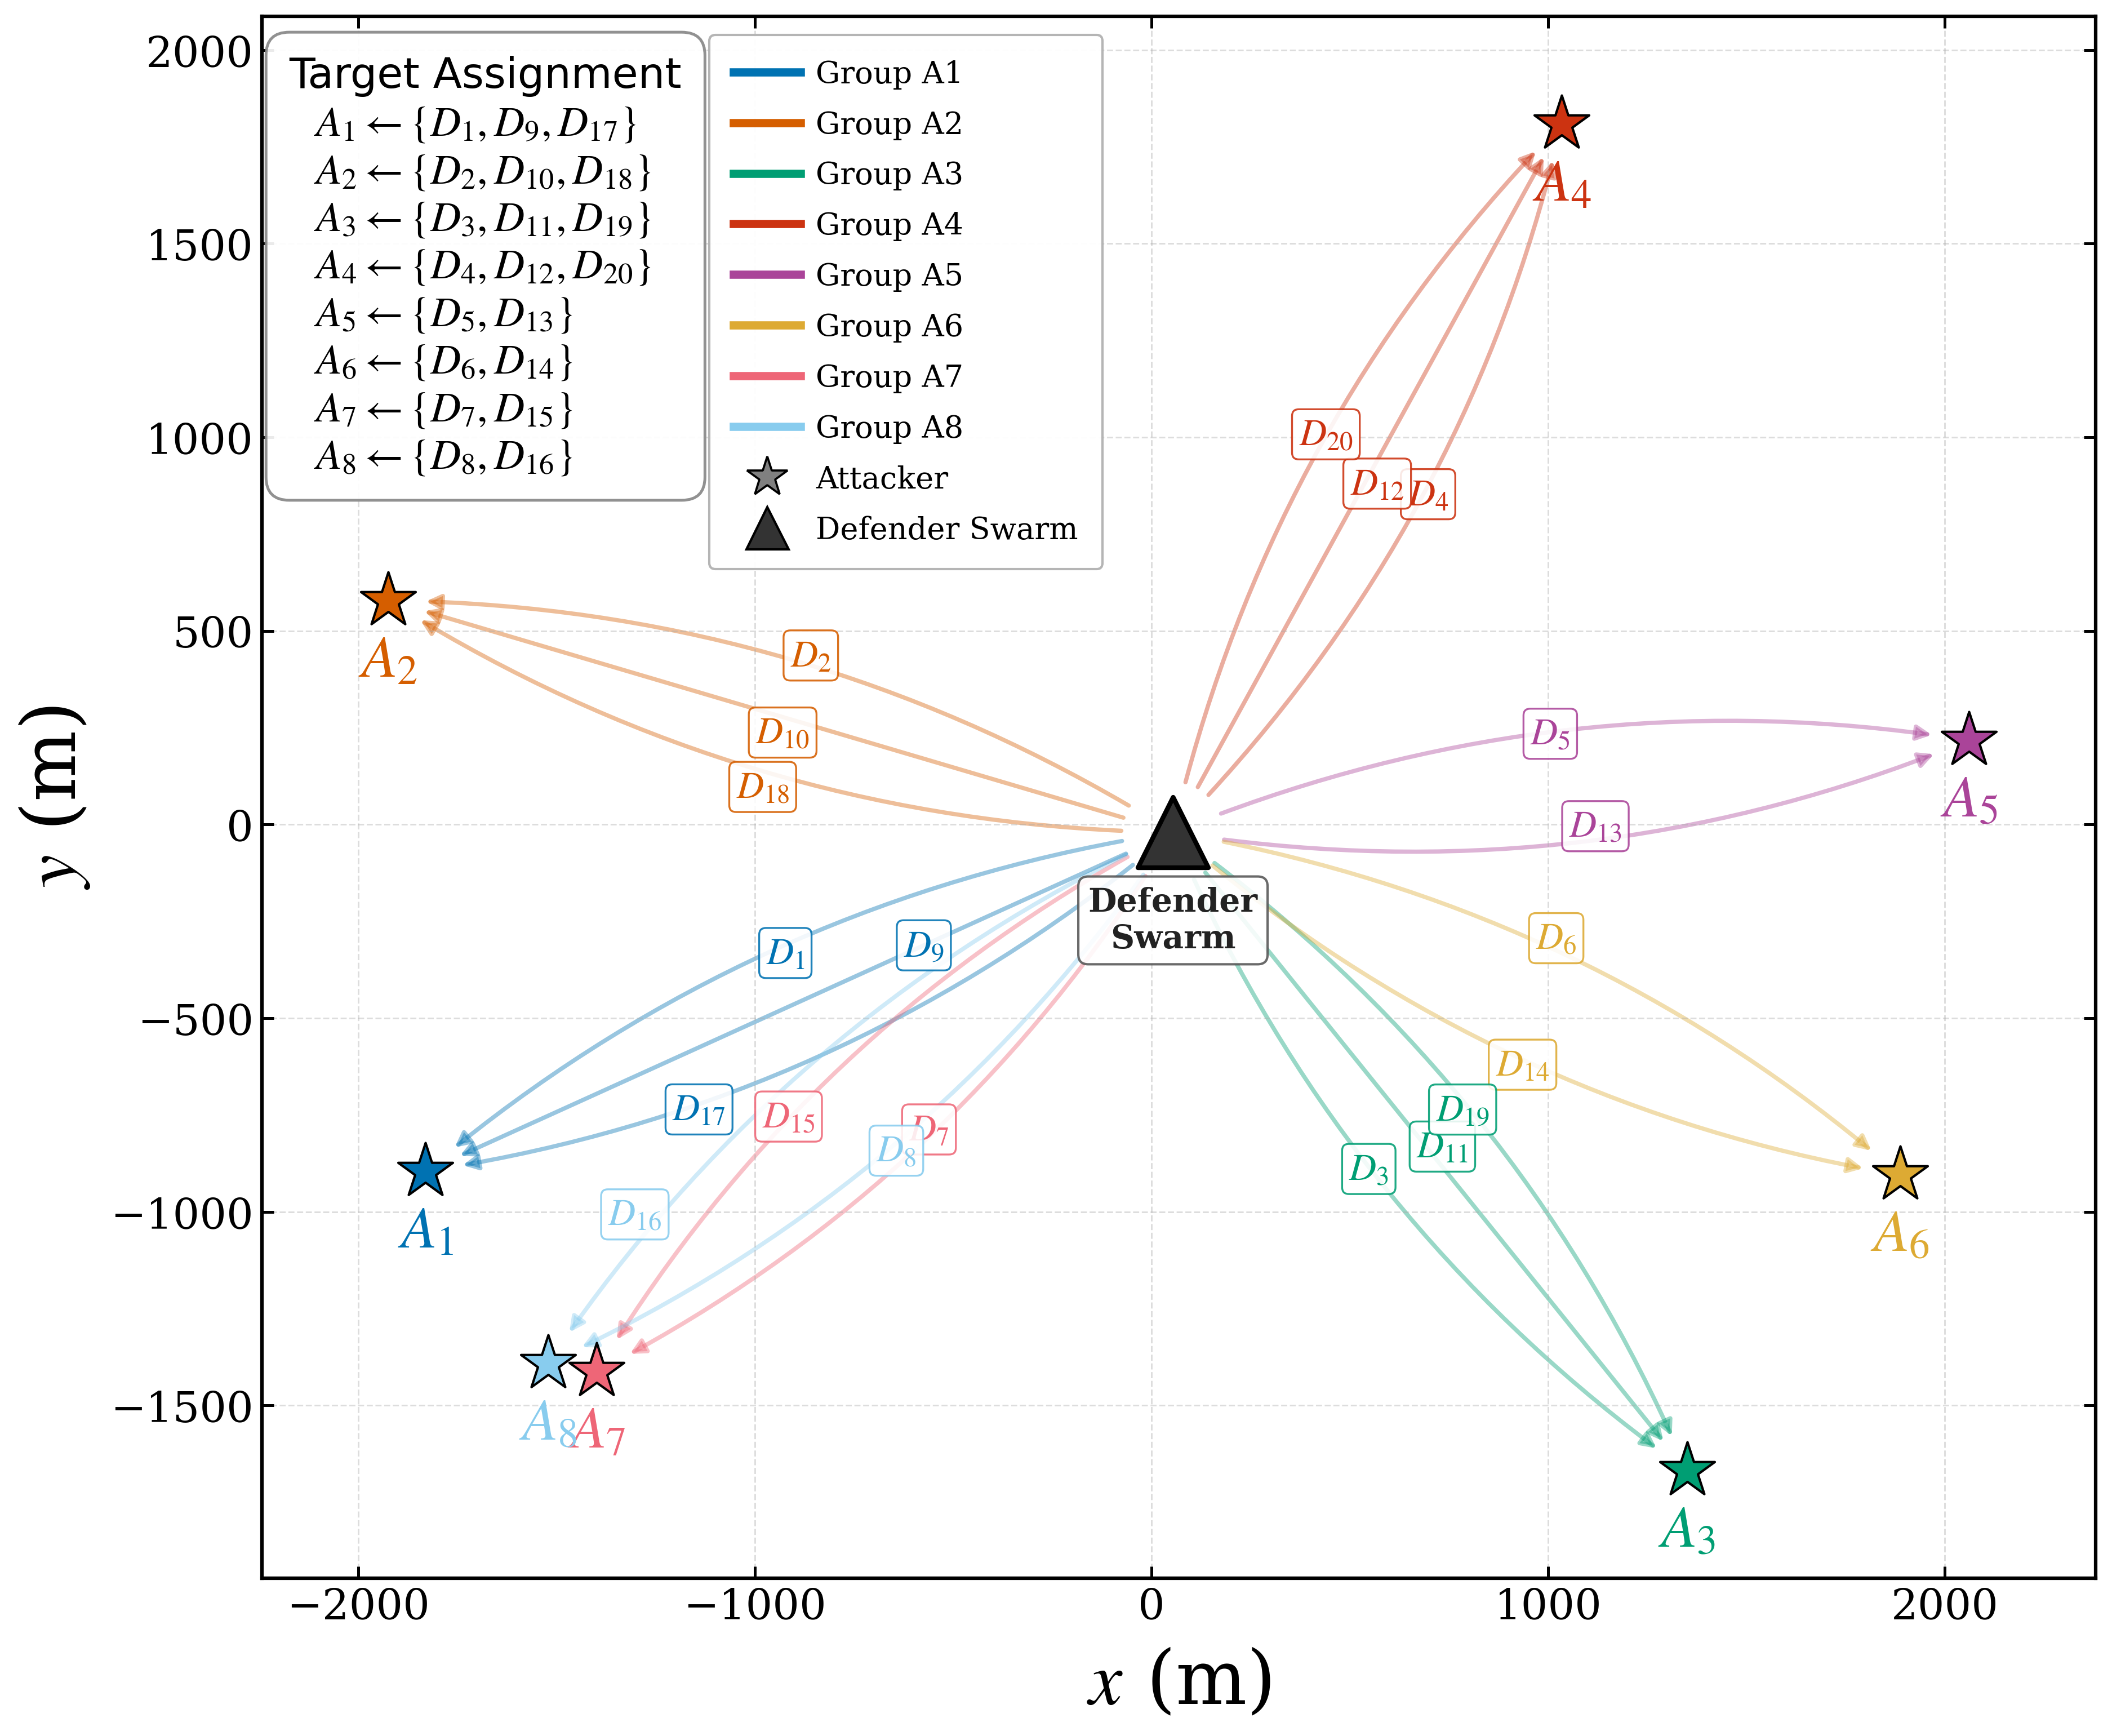
\includegraphics[width=3.2in]{target_assignment_topology.png}
\caption{Visualized spatial topology of the target assignment results.}
\label{fig:assignment_topology}
\end{figure}








\subsection{RL Model Training and Convergence Analysis}
\label{subsec:training}

To evaluate the learning efficiency and robustness of the proposed ART-MAPPO, comparative training experiments were conducted against standard MAPPO, IPPO, IA2C, and IQL. All models were trained over 10,000 episodes with a maximum horizon of 25 steps per episode. To ensure statistical significance and eliminate the bias of favorable network initialization, all learning curves in Fig.~\ref{fig:training_convergence} are averaged across 5 independent random seeds, with the shaded regions denoting the standard deviation.

As illustrated in Fig.~\ref{fig:training_convergence}(a), ART-MAPPO demonstrates a superior learning paradigm, achieving the highest asymptotic normalized reward of $8.97 \pm 0.64$ (averaged over the final 500 episodes). This represents a notable performance improvement of 8.2\%, 12.3\%, 14.4\%, and 29.8\% over IQL, MAPPO, IPPO, and IA2C, respectively. The advantage of ART-MAPPO is particularly pronounced during the intermediate training phase. By episode 4,000, ART-MAPPO establishes a significant performance leap, outperforming standard MAPPO by 43.6\% and IQL by 16.6\%, highlighting its ability to rapidly escape local optima early in the training process.

Furthermore, the proposed method exhibits accelerated convergence alongside enhanced training stability. When evaluated on a 100-episode smoothed curve, ART-MAPPO reaches 90\% of its optimal asymptotic performance by episode 5,591. In contrast, the most competitive baseline, IQL, requires 6,477 episodes (a 13.7\% delay), while standard MAPPO lags significantly, requiring 7,654 episodes. Regarding algorithmic stability, ART-MAPPO maintains a tight variance across random seeds ($\sigma = 0.64$), whereas standard MAPPO exhibits a standard deviation of 1.34 (approximately twice as large). This confirms that the proposed enhancements effectively mitigate the high-variance gradient updates typical in multi-agent policy-based methods.

These macroscopic performance gains are directly supported by the network-level metrics. The critic loss (Fig.~\ref{fig:training_convergence}(b)) of ART-MAPPO converges to the lowest steady-state error with minimal oscillation, a direct consequence of the dual-clip mechanism and adaptive KL penalty. Concurrently, the policy entropy (Fig.~\ref{fig:training_convergence}(c)) demonstrates an optimal, gradual decay trajectory, validating that the trust-modulated exploration mechanism successfully balances early-stage extensive state-space exploration with late-stage strict policy exploitation.

\DIFaddbegin \DIFadd{It should be emphasized that the convergence discussed here is empirical training
convergence rather than a global optimality guarantee for the nonconvex MARL problem. In
particular, ART-MAPPO inherits the practical convergence interpretation of PPO-style policy
gradient methods: a stable learning process is indicated by a saturating reward curve, bounded
inter-seed variance, a nondivergent critic loss, and a gradually decreasing policy entropy.
The dual-clip objective and adaptive KL penalty do not prove convergence to the global
optimum; instead, they restrict the policy update magnitude and reduce destructive policy
oscillations caused by large importance-sampling ratios. Therefore, the convergence claim for
ART-MAPPO should be understood as statistically validated stability and asymptotic performance
under the tested training settings, supported by the five-seed learning curves and the
network-level diagnostics in Fig.~\ref{fig:training_convergence}.
}

\DIFaddend \begin{figure}[!t]
\centering
\subfloat[Training Reward]{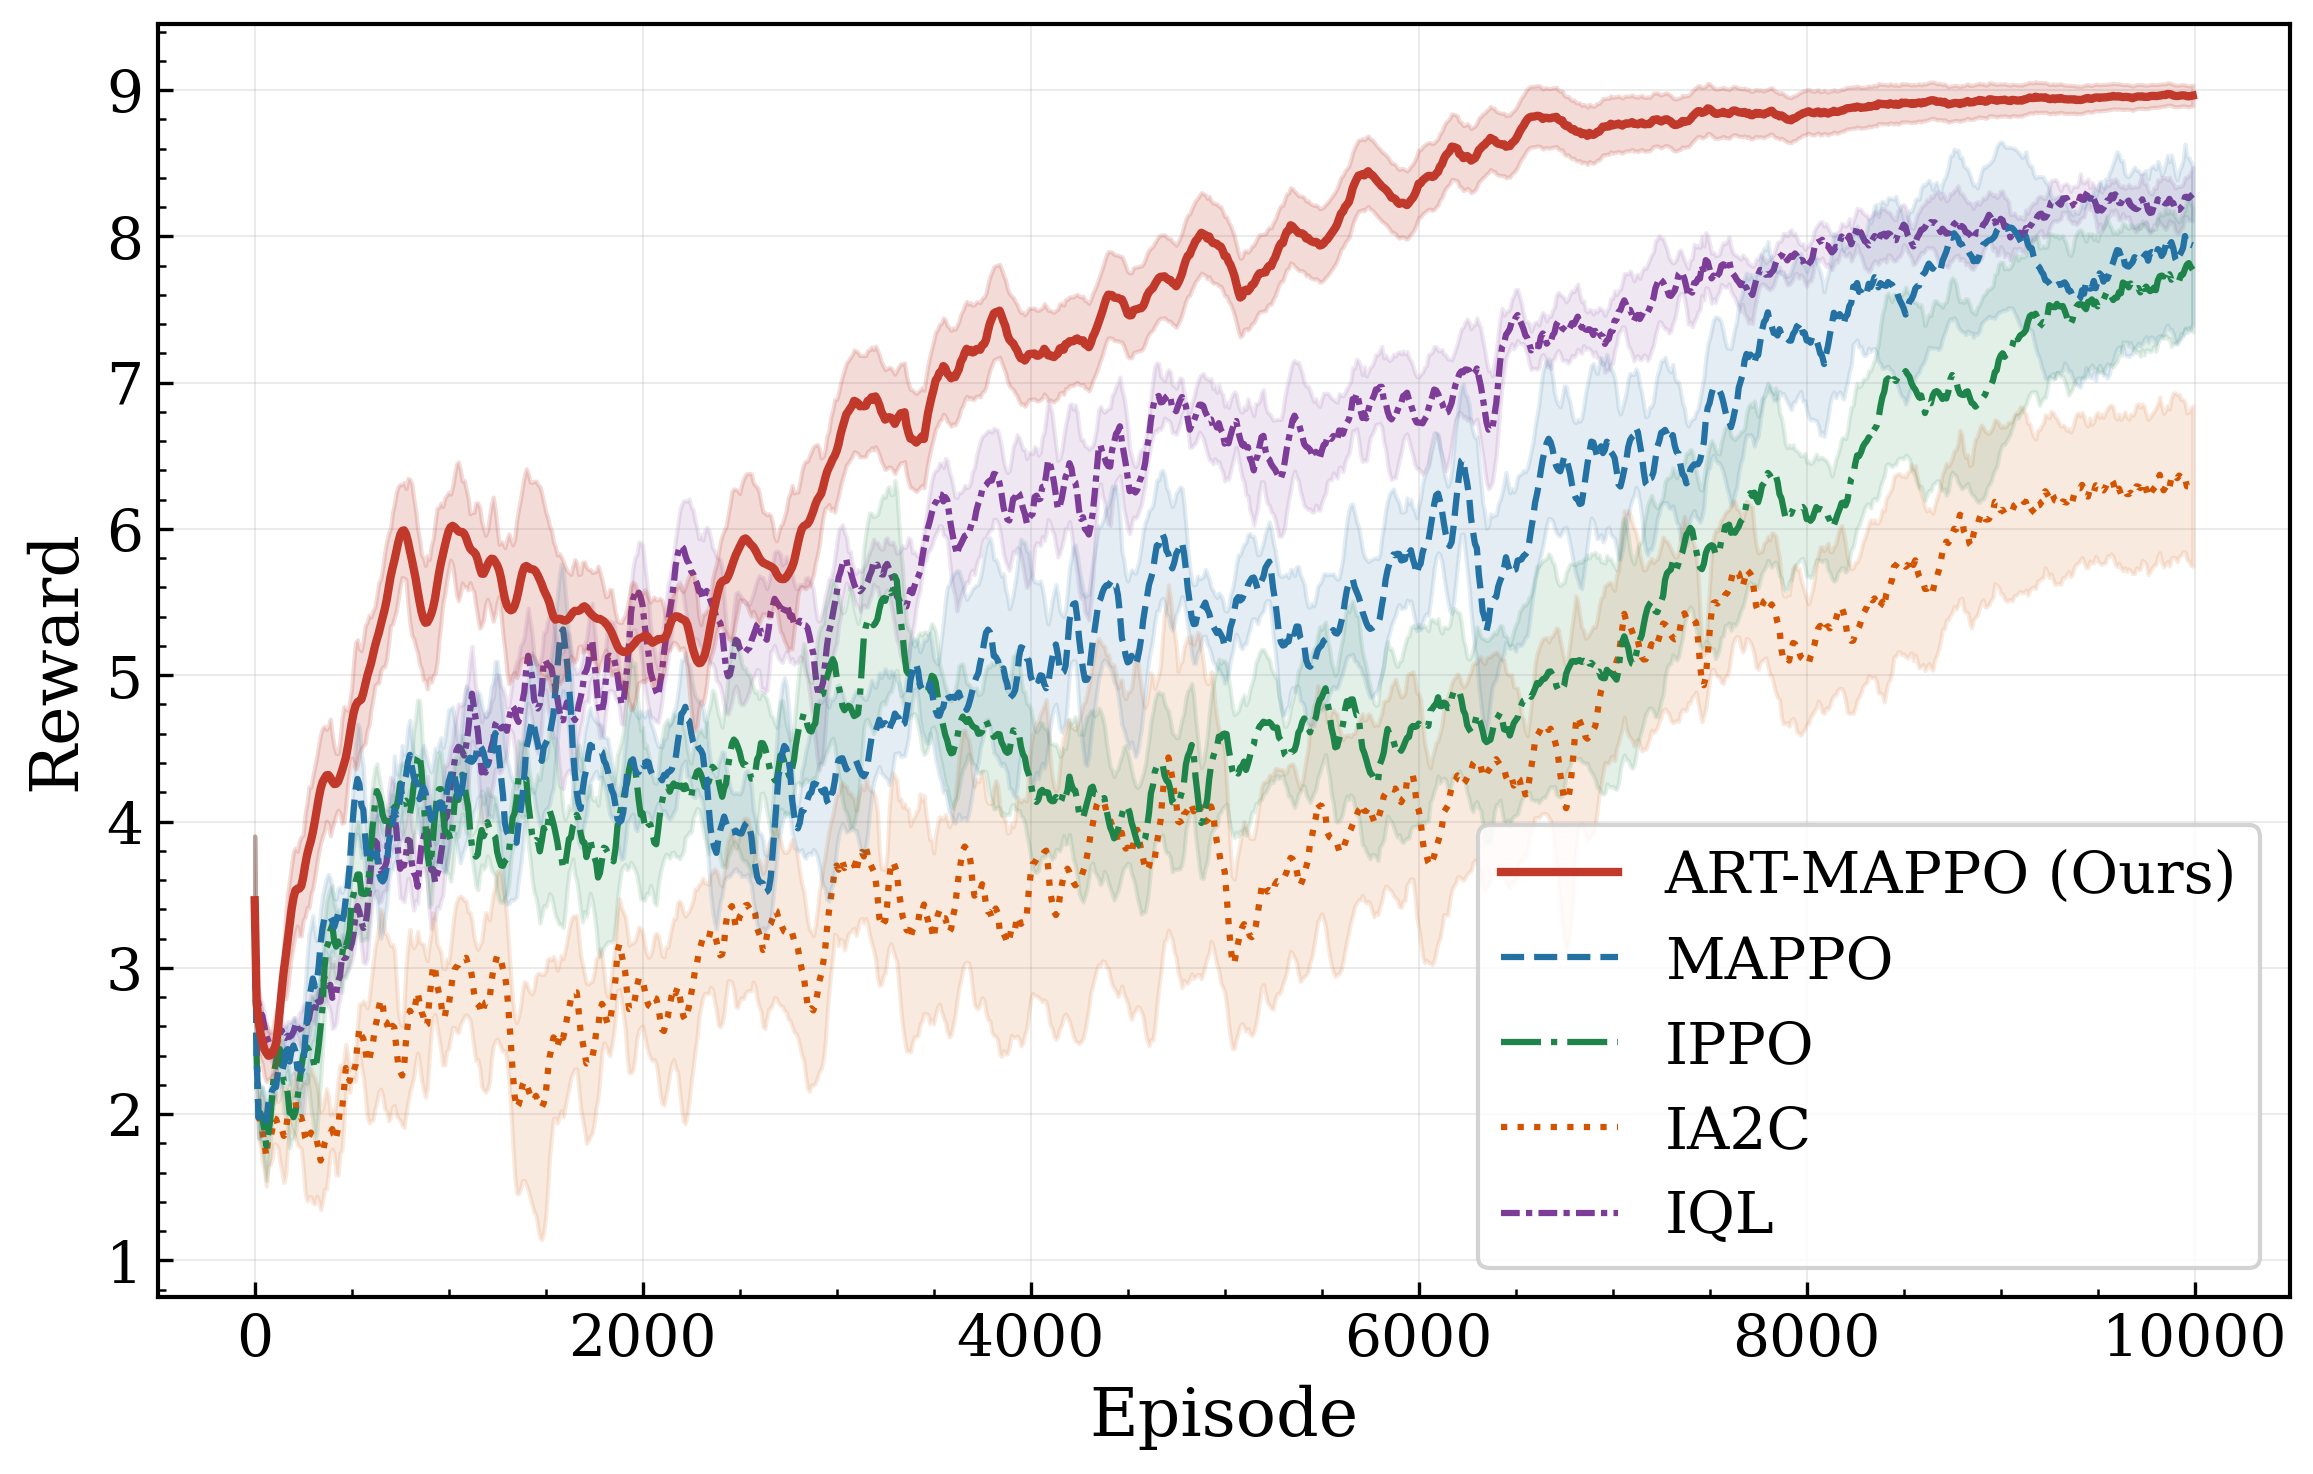
\includegraphics[width=3.0in]{fig_a_reward.png}}
\hfill
\subfloat[Critic Loss]{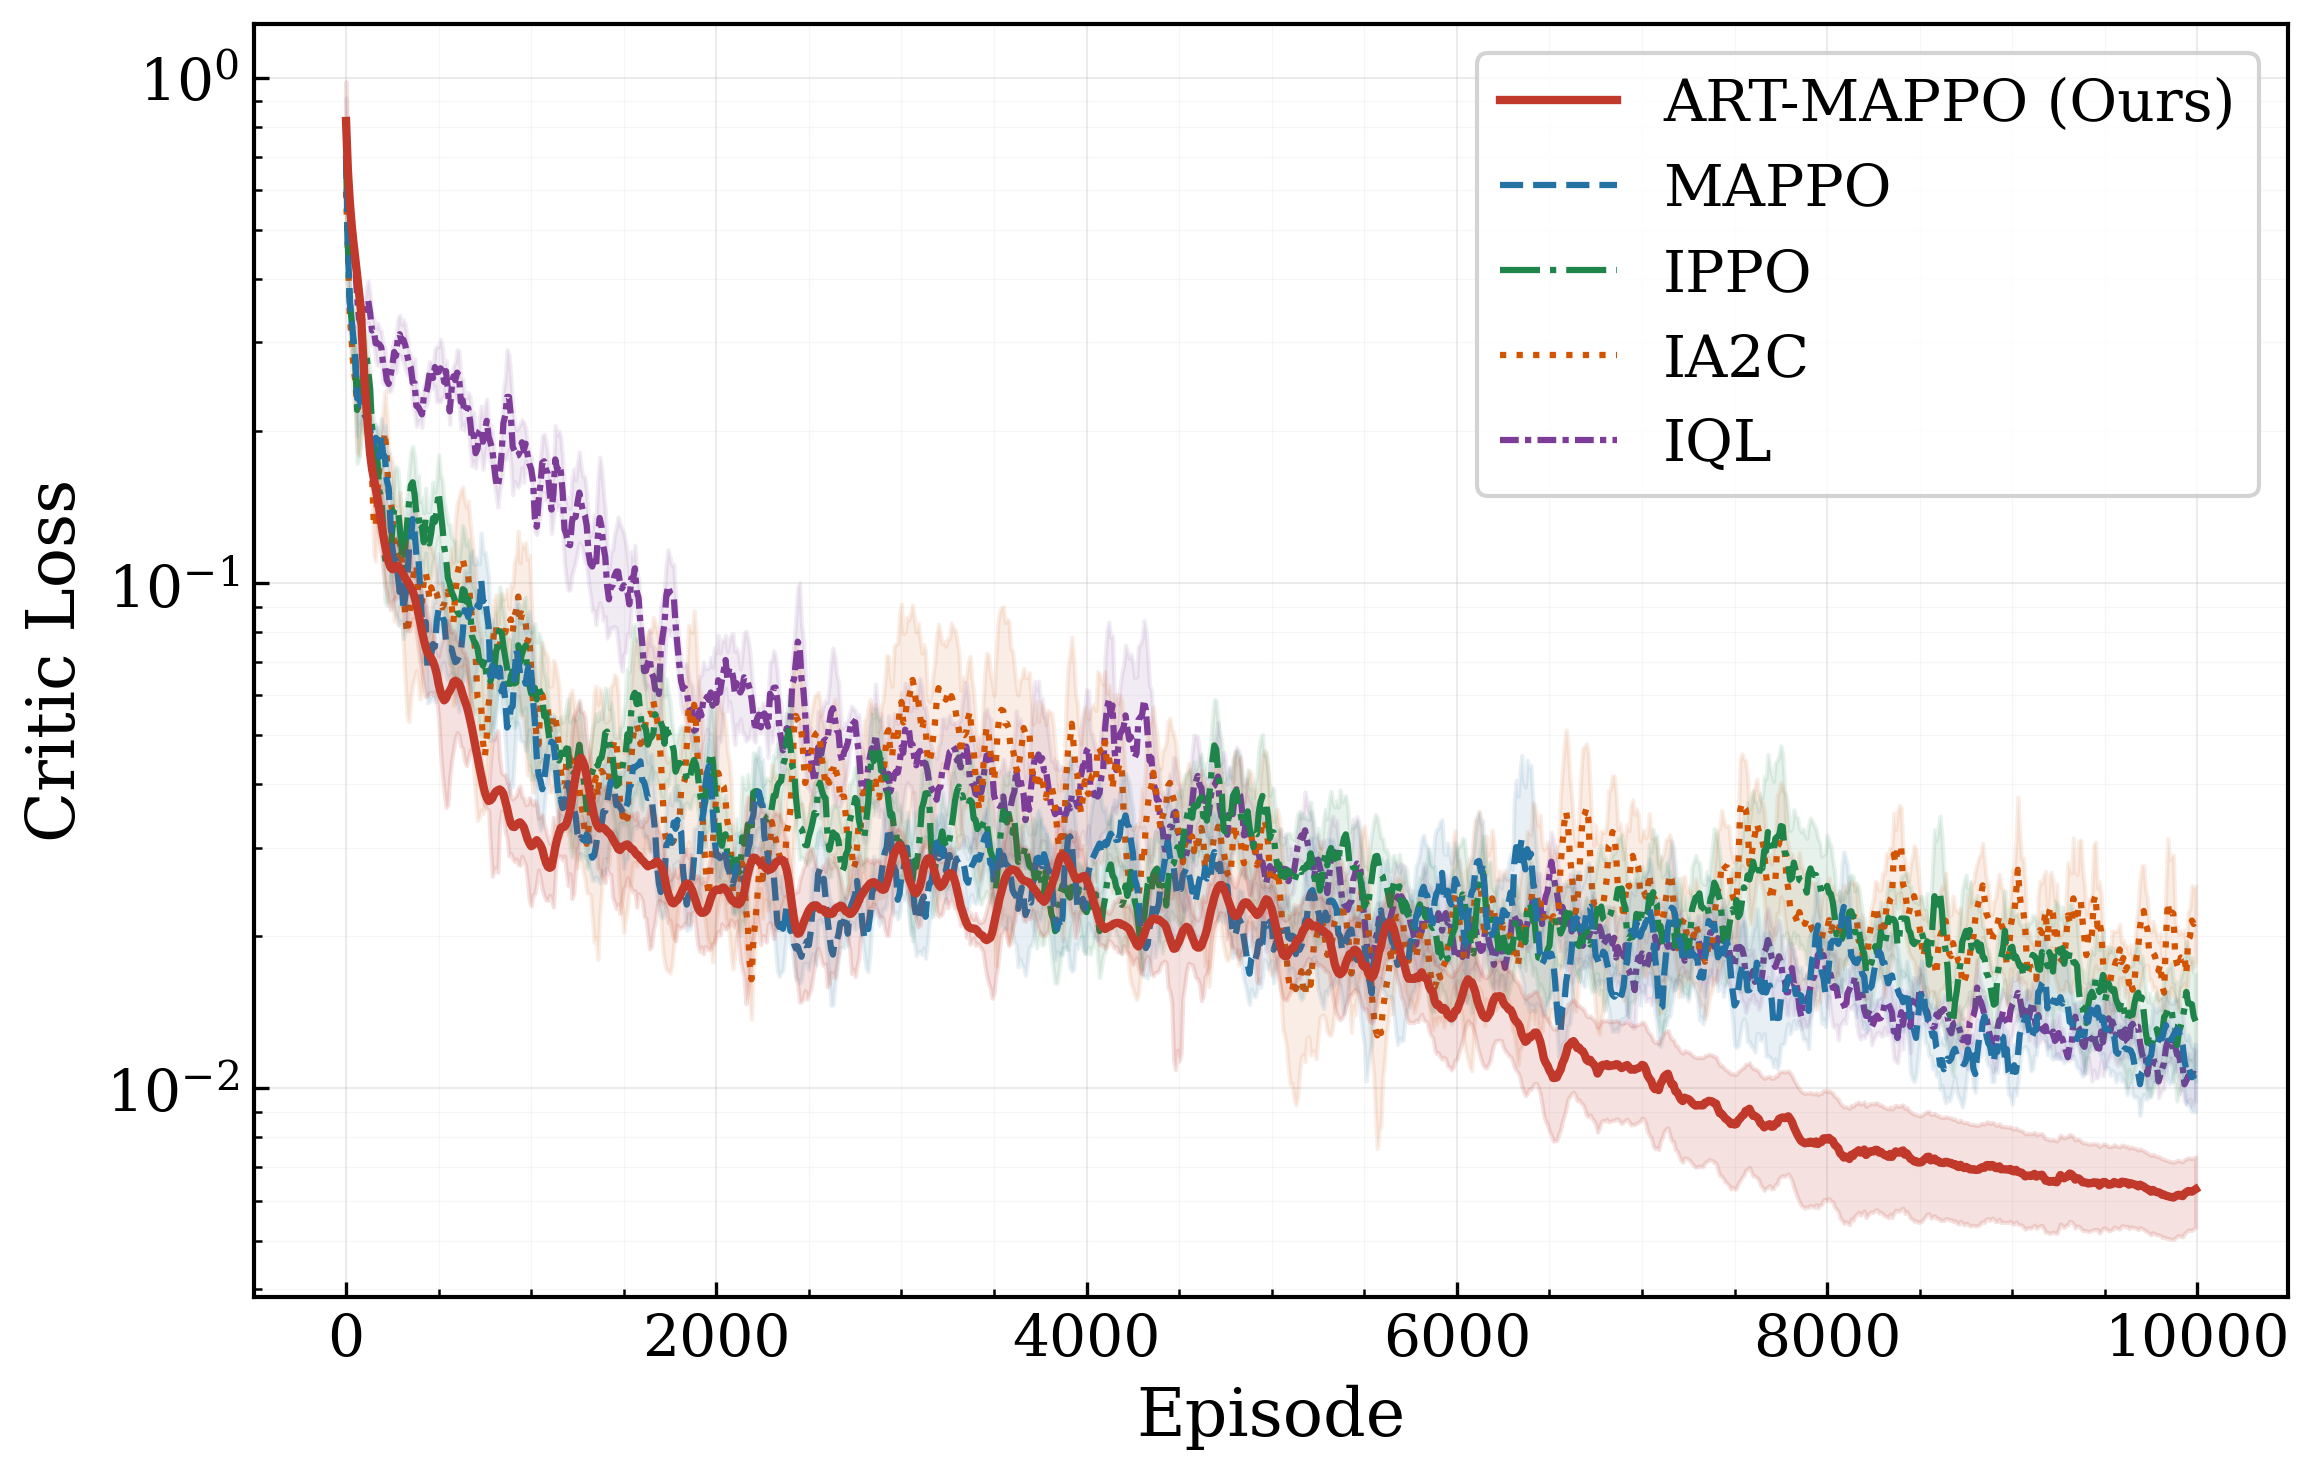
\includegraphics[width=3.0in]{fig_b_critic_loss.png}}
\hfill
\subfloat[Policy Entropy]{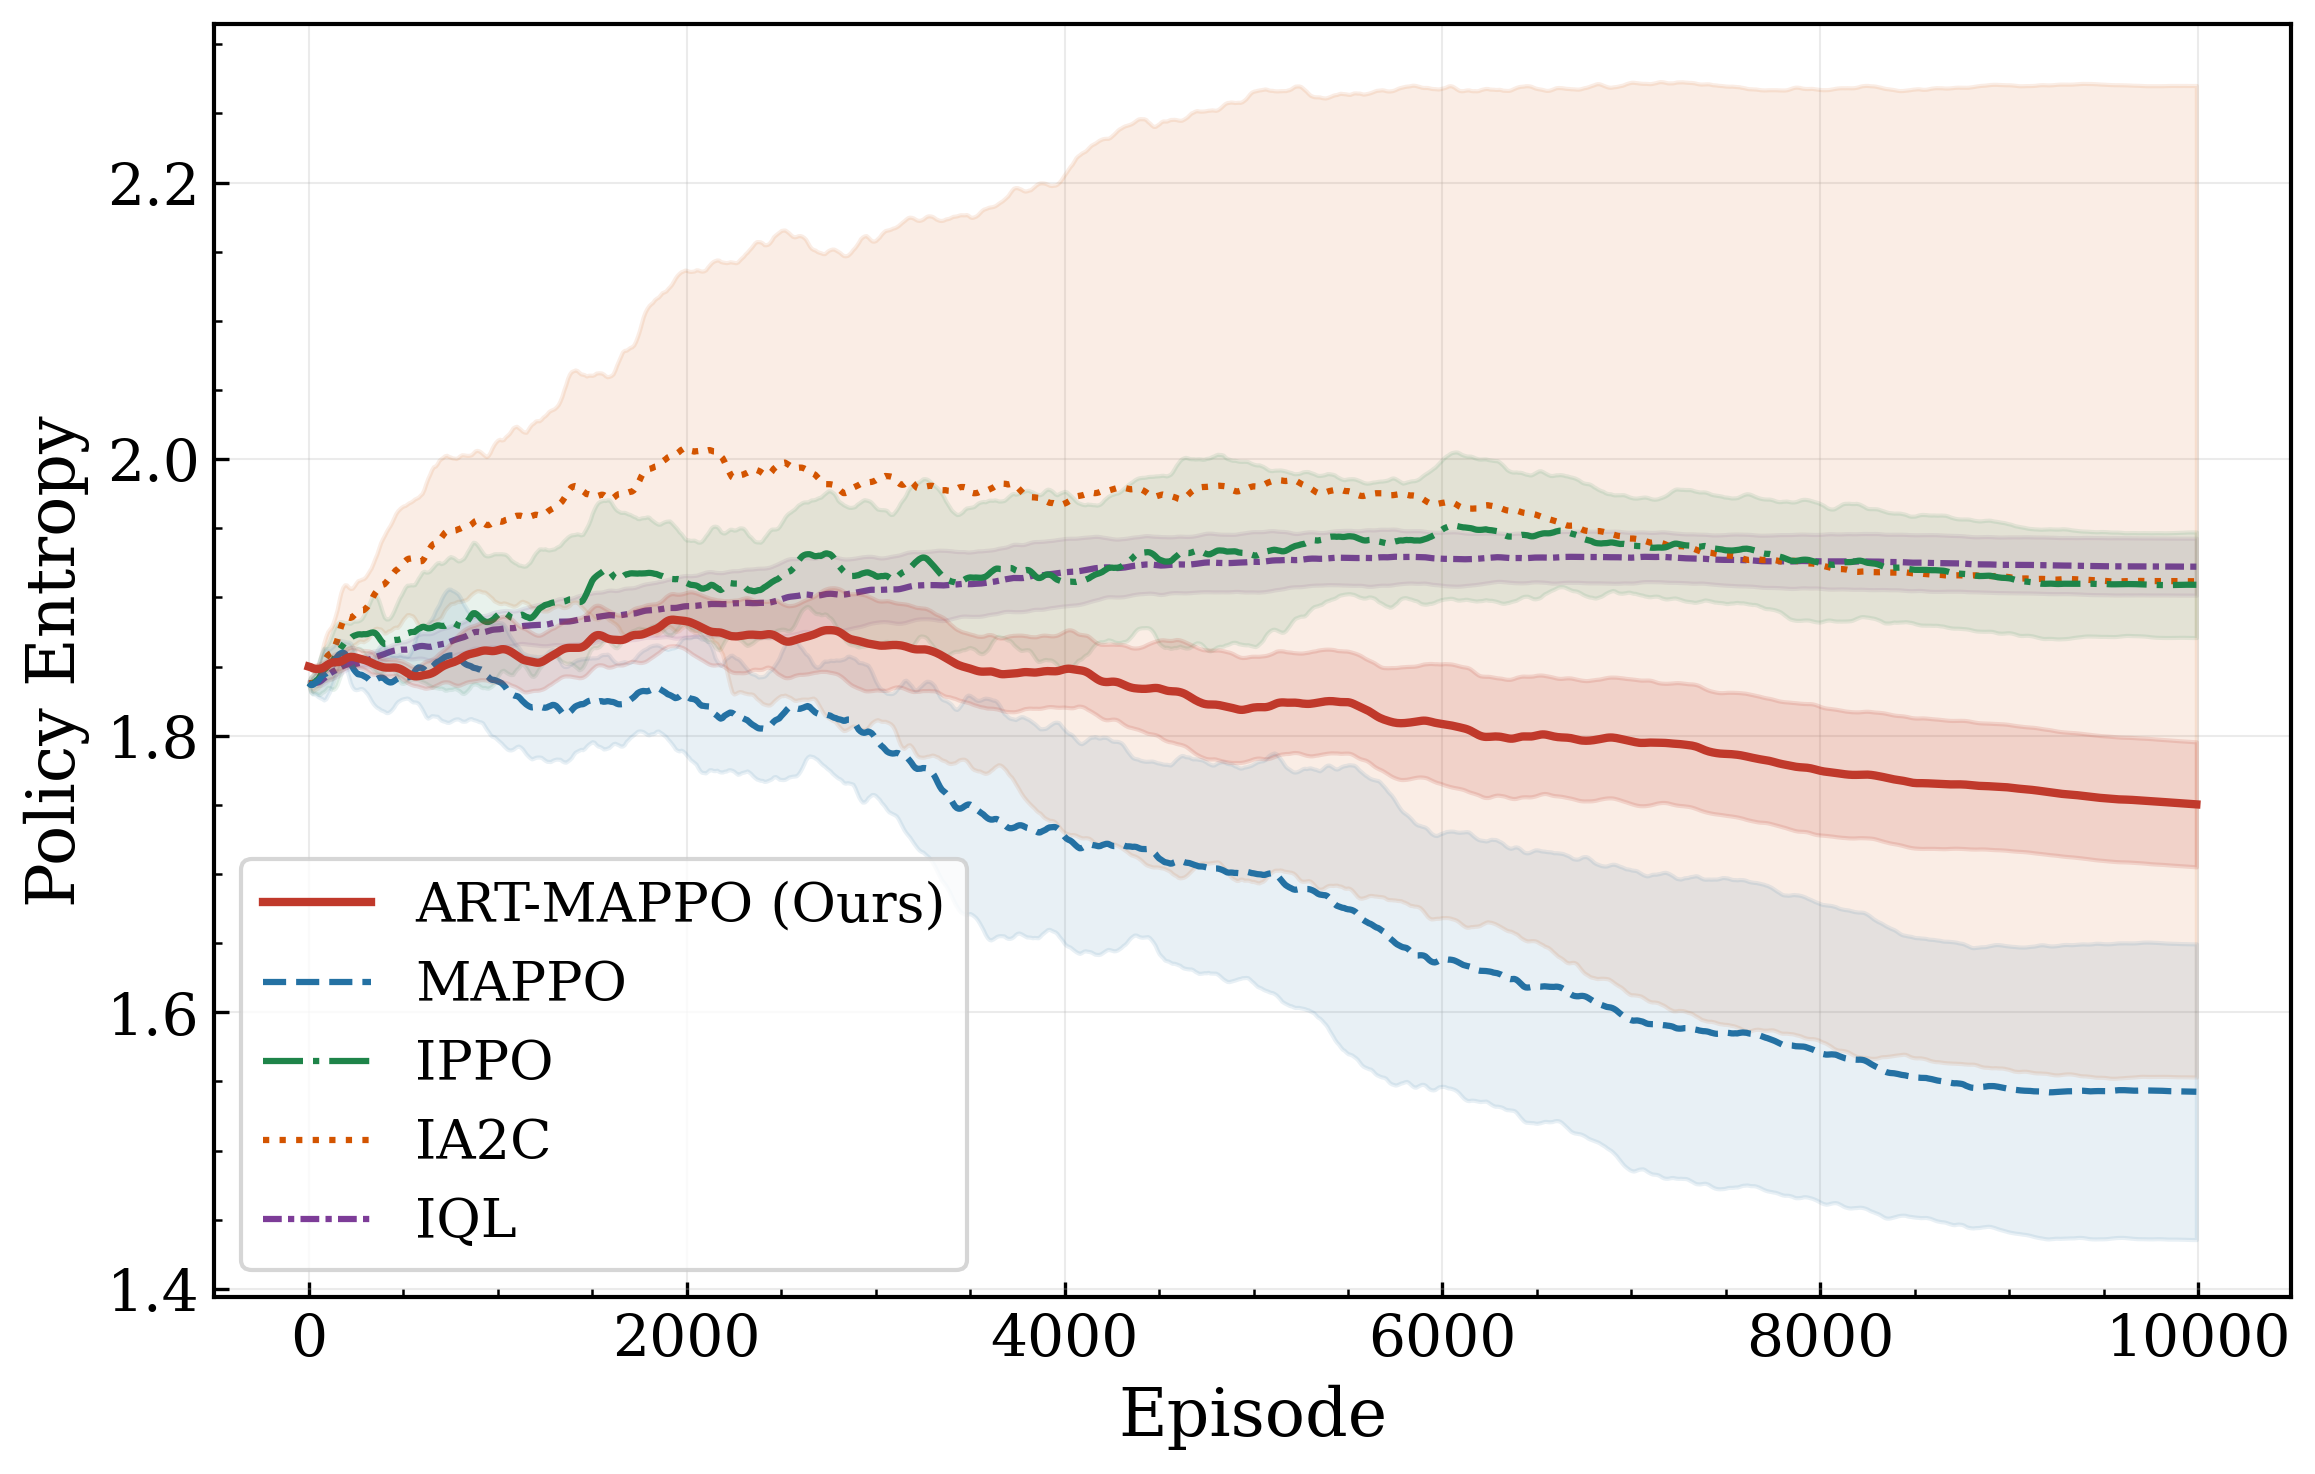
\includegraphics[width=3.0in]{fig_c_entropy.png}}
\caption{Comparative training curves of ART-MAPPO and baseline algorithms over 10,000 episodes. Solid lines and shaded regions represent the mean and standard deviation across 5 independent random seeds, respectively. Notably, ART-MAPPO achieves the highest asymptotic reward (+12.3\% over standard MAPPO) and the fastest convergence rate (reaching 90\% optimality by episode 5,591), while demonstrating significantly enhanced training stability.}
\label{fig:training_convergence}
\end{figure}




%DIF < %%%-------------------------------------------------------------------------------------------
\DIFaddbegin \subsection{\DIFadd{Offline Reward-Function Sensitivity Analysis}}
\label{subsec:offline_reward_sensitivity}

\DIFadd{We further examine the sensitivity of the reward definition to three representative weights
and one nonlinear shaping hyperparameter. The implementation keys
$w_{\mathrm{hit}}$, $w_{\mathrm{coord}}$, and $w_{\mathrm{energy}}$ correspond to the
terminal, coordination, and effort weights $\lambda_h$, $\lambda_c$, and $\lambda_u$ in
}\eqref{eq:reward_function}\DIFadd{, respectively, while
$\alpha_d\equiv d_{\mathrm{ref}}^{-1}$ determines the exponential distance-reward decay.
Their nominal values are $w_{\mathrm{hit}}=200$,
$w_{\mathrm{coord}}=18$, $w_{\mathrm{energy}}=0.005$, and
$\alpha_d=2\times10^{-4}\,\mathrm{m}^{-1}$. Each parameter is independently multiplied by
$\kappa\in\{0.50,0.75,1.00,1.25,1.50\}$ while all other reward parameters remain nominal.
}

\DIFadd{This experiment isolates reward-function sensitivity from policy adaptation. Specifically,
the trained nominal ART-MAPPO policies are frozen, and no gradient, optimizer step, or policy
update is performed. We collect 100 stochastic evaluation episodes (50 per case) and store
the distance, time-to-go mismatch, three-axis control effort, and first-hit events. In every
recorded episode, all 20 defenders reach their assigned targets and all eight attackers are
intercepted, so the sparse hit contribution is evaluated on successful trajectories without
changing any event indicator. Every
parameter setting is then evaluated by recomputing the reward on these }\emph{\DIFadd{same}} \DIFadd{state--action
trajectories. For episode $e$, the normalized cumulative-reward variation is
}\begin{equation}
\DIFadd{\label{eq:normalized_reward_sensitivity}
\Delta G_{e}^{\mathrm{norm}}(\kappa;\theta)=
\frac{G_e(\kappa\theta_0)-G_e(\theta_0)}{\sum_t|r_e(t;\theta_0)|+10^{-8}},
}\end{equation}
\DIFadd{where $G_e(\theta)=\sum_t r_e(t;\theta)$. Thus, Fig.~\ref{fig:reward_sensitivity}
characterizes the mapping $\theta\mapsto r(s,a;\theta)$ for fixed trajectories rather than
the performance of policies retrained under altered rewards.
}

\begin{figure*}[!t]
\centering
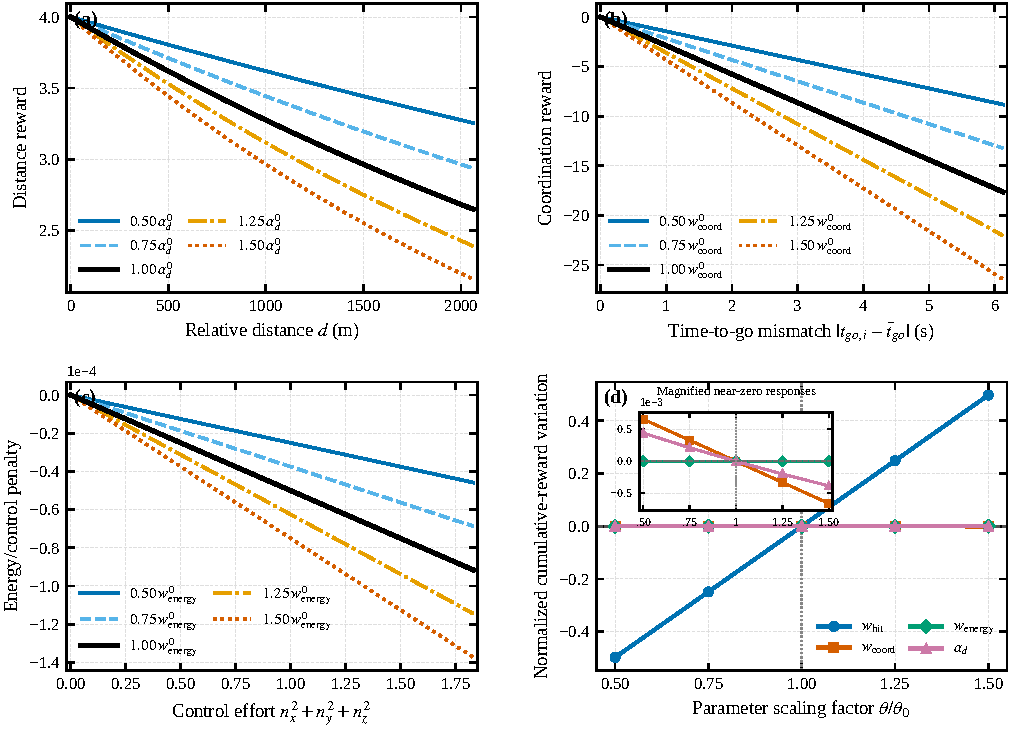
\includegraphics[width=7.0in]{reward_sensitivity_v10.pdf}
\caption{\DIFaddFL{Sensitivity of the reward function to representative weighting and shaping
parameters. (a) Distance reward versus relative distance under variations of $\alpha_d$.
(b) Coordination reward versus time-to-go mismatch under variations of
$w_{\mathrm{coord}}$. (c) Energy/control penalty versus three-axis control effort under
variations of $w_{\mathrm{energy}}$. (d) Mean normalized cumulative-reward variation on 100
fixed ART-MAPPO evaluation trajectories; shaded regions denote 95\% confidence intervals,
and the inset magnifies the three near-zero responses.}}
\label{fig:reward_sensitivity}
\end{figure*}

\DIFadd{The component-level responses in Figs.~\ref{fig:reward_sensitivity}(a)--(c) agree with the
reward definition. Reducing $\alpha_d$ to $1.0\times10^{-4}\,\mathrm{m}^{-1}$ extends the
distance-reward e-folding range from the nominal 5.0\,km to 10.0\,km, whereas increasing it
to $3.0\times10^{-4}\,\mathrm{m}^{-1}$ contracts that range to 3.33\,km. The resulting
separation of the curved profiles over the observed 0--2.063\,km range confirms a nonlinear,
rather than merely amplitude-scaled, change in the reward landscape. In contrast, the
coordination and effort terms change linearly with their outer weights. At the nominal
setting, the coordination slope is
$-w_{\mathrm{coord}}\alpha_c=-2.88$ reward units per second of time-to-go mismatch; the
$0.5$--$1.5\times$ sweep changes this slope from $-1.44$ to $-4.32$. Similarly, the
effort-penalty slope changes from $-2.5\times10^{-5}$ to
$-7.5\times10^{-5}$ per unit of $n_x^2+n_y^2+n_z^2$.
}

\DIFadd{For a dimensionless comparison around the nominal point, we use
}\begin{equation}
\DIFadd{\label{eq:local_reward_sensitivity}
S_{\theta}=\frac{1}{100}\sum_{e=1}^{100}
\frac{\left|\Delta G_e^{\mathrm{norm}}(1.25;\theta)
-\Delta G_e^{\mathrm{norm}}(0.75;\theta)\right|}{0.5}.
}\end{equation}
\DIFadd{The resulting indices are $0.995913$ for $w_{\mathrm{hit}}$, $0.001317$ for
$w_{\mathrm{coord}}$, $0.000823$ for $\alpha_d$, and
$1.35\times10^{-8}$ for $w_{\mathrm{energy}}$. The terminal weight is therefore the
dominant cumulative-reward sensitivity for these successful fixed trajectories: the mean
nominal hit contribution is $8.80\times10^6$, compared with a mean total return of
$8.825\times10^6$. The coordination and distance-shaping parameters have substantially
smaller but clearly resolved effects around the nominal point. In particular, increasing
$w_{\mathrm{coord}}$ steepens the penalty for any given arrival-time mismatch, while
$\alpha_d$ produces the expected asymmetric nonlinear response in
Fig.~\ref{fig:reward_sensitivity}(d). The very small effort index reflects its small nominal
coefficient and the bounded control effort on the evaluated trajectories; it does not imply
that high control effort is unpenalized, because panel (c) still shows the proportional
increase in the instantaneous penalty. Finally, the variation is exactly zero at
$\kappa=1$ for all four parameters, and all confidence intervals are computed over the same
100 episodes, confirming a controlled one-factor-at-a-time comparison.
}\DIFaddend 

\subsection{Cooperative Interception against Maneuvering Targets}
\label{subsec:cases}

Based on the optimal assignment topology, we evaluate \DIFdelbegin \DIFdel{the terminal cooperative guidance
performance against }\DIFdelend \DIFaddbegin \DIFadd{three-dimensional cooperative guidance
in }\DIFaddend two maneuvering scenarios\DIFdelbegin \DIFdel{, each benchmarked against classical PN}\DIFdelend \DIFaddbegin \DIFadd{. ART-MAPPO and the capacity-matched PN reference use the same
initial states, target assignment, hit radius, speed limits, load-factor envelope, and other
scenario settings described in Section~\ref{subsec:setup}. For each
method and case, we report the three-dimensional trajectory, its horizontal projection, all
three load commands and their associated attitude/speed responses, time-to-go histories, and
terminal arrival-time differences}\DIFaddend .

\subsubsection{Case~1: Interception against Evasive Maneuvering Targets}

In \DIFdelbegin \DIFdel{this scenario}\DIFdelend \DIFaddbegin \DIFadd{Case~1}\DIFaddend , the attacking UAVs \DIFdelbegin \DIFdel{($A_{\text{UAV}}$) }\DIFdelend initially execute a \DIFdelbegin \DIFdel{constant-$g$ }\DIFdelend \DIFaddbegin \DIFadd{constant-load }\DIFaddend evasive maneuver and transition
to \DIFdelbegin \DIFdel{proportional navigation (PN ) }\DIFdelend \DIFaddbegin \DIFadd{PN }\DIFaddend guidance after 15\,s. \DIFdelbegin \DIFdel{The defending swarm is tasked with neutralizing these highly dynamic threats utilizing the pre-computed assignment topology}\DIFdelend \DIFaddbegin \DIFadd{This creates simultaneous horizontal and vertical closing demands
while the defenders must preserve the assignment groups and coordinate their terminal arrival
times}\DIFaddend .

\DIFaddbegin \emph{\DIFadd{1) ART-MAPPO:}} \DIFaddend Fig.~\DIFdelbegin \DIFdel{\ref{fig:case1_mappo_traj} illustrates the 2D engagementtrajectories generated by the proposed ART-MAPPO algorithm. Guided by the intelligent policy, the defending swarm effectively divides into eight coordinated combat units. Despite the evasive maneuvers of the targets, ART-MAPPO generates remarkably smooth and direct pursuit curves, enabling all interceptors to successfully converge on their respective targets without unnecessary detours}\DIFdelend \DIFaddbegin \DIFadd{\ref{fig:case1_mappo_traj_3d} shows the complete spatial
engagement. Starting below the attackers, the defenders climb from the defended region and
close on the eight elevated target trajectories. The horizontal projection in
Fig.~\ref{fig:case1_mappo_traj_xy} preserves the original plan-view interpretation and shows
that all 20 defenders converge on the targets specified by the assignment topology}\DIFaddend .

\begin{figure}[!ht]
\centering
\DIFdelbeginFL %DIFDELCMD < 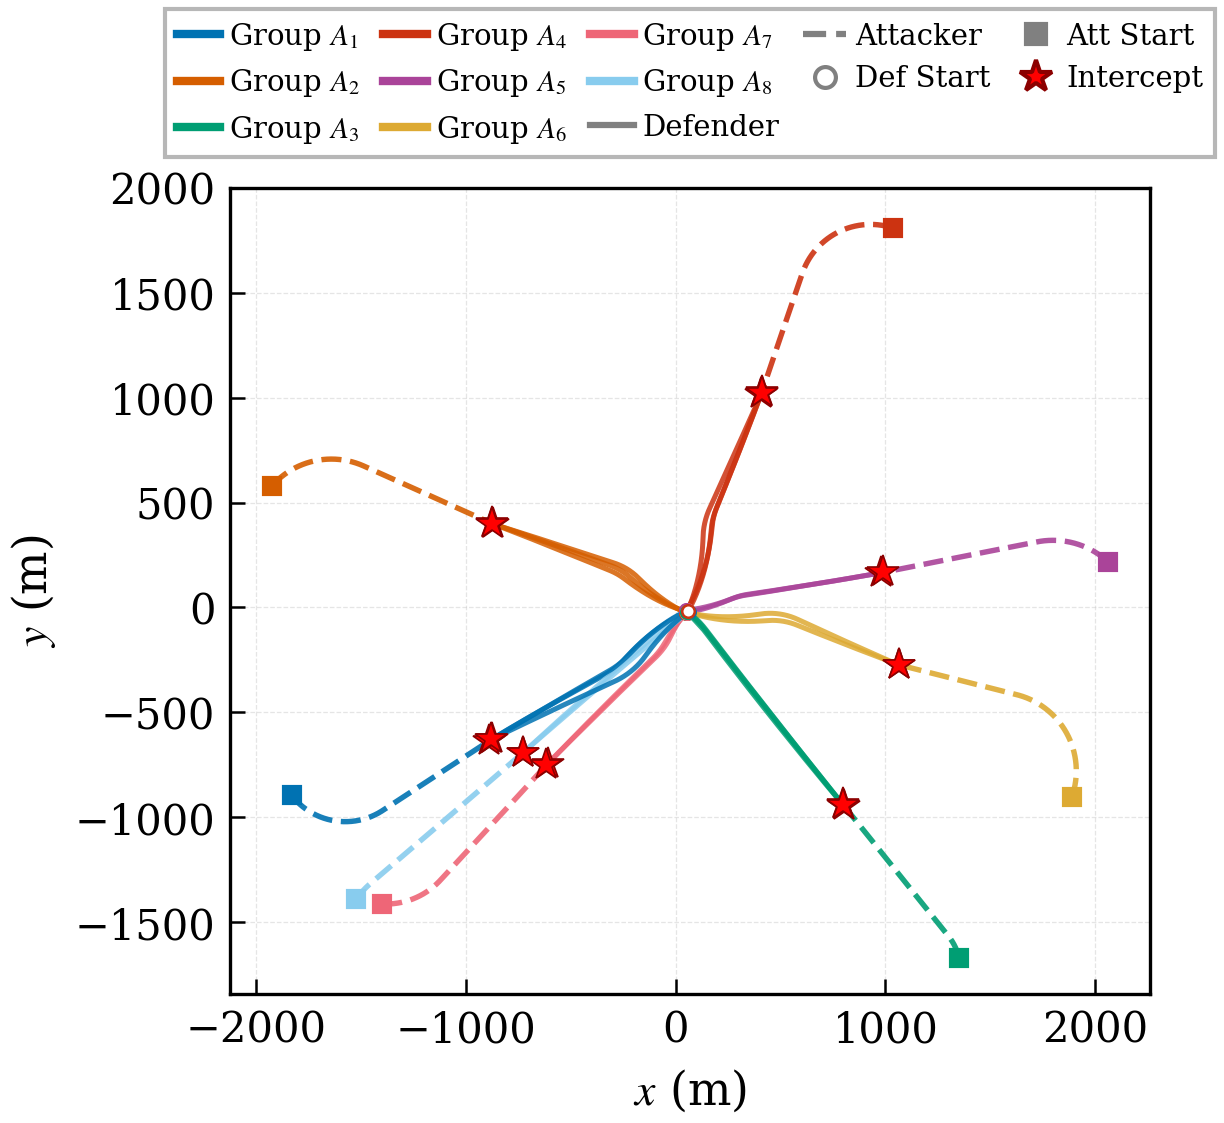
\includegraphics[width=3.2in]{mappo_nopn_trajectory.png}
%DIFDELCMD < %%%
\DIFdelendFL \DIFaddbeginFL 
\includegraphics[width=3.15in]{../new_sim_fig/figures_v10/mappo/mappo_nopn_trajectory_3d.png}
\DIFaddendFL \caption{\DIFdelbeginFL \DIFdelFL{Engagement }\DIFdelendFL \DIFaddbeginFL \DIFaddFL{Three-dimensional engagement }\DIFaddendFL trajectories of the defending swarm using ART-MAPPO in
Case~1.}
\DIFdelbeginFL %DIFDELCMD < \label{fig:case1_mappo_traj}
%DIFDELCMD < %%%
\DIFdelendFL \DIFaddbeginFL \label{fig:case1_mappo_traj_3d}
\DIFaddendFL \end{figure}

\DIFdelbegin \DIFdel{To deeply analyze the operational efficiency and constraint adherence of the proposed method, Fig.~\ref{fig:case1_mappo_kine} presents the comprehensive kinematic and control profiles of ART-MAPPO. Most critically, the normal
acceleration (}\DIFdelend \DIFaddbegin \begin{figure}[!ht]
\centering

\includegraphics[width=3.15in]{../new_sim_fig/figures_v10/mappo/mappo_nopn_trajectory.png}
\caption{\DIFaddFL{Horizontal projection of the ART-MAPPO engagement trajectories in Case~1.}}
\label{fig:case1_mappo_traj_xy}
\end{figure}

\DIFadd{The corresponding command and state histories are separated into three physically related
pairs in Figs.~\ref{fig:case1_mappo_yaw}--\ref{fig:case1_mappo_axial}. The horizontal normal
command }\DIFaddend $n_y$ \DIFdelbegin \DIFdel{) profile in Fig.~\ref{fig:case1_mappo_kine}(a) highlights the safety and robustness of the learned policy: }\DIFdelend \DIFaddbegin \DIFadd{and heading $\gamma_D$ form the yaw-plane response, while $n_z$ and pitch
$\theta_D$ show the vertical response that is absent from a planar model. }\DIFaddend ART-MAPPO \DIFdelbegin \DIFdel{strictly bounds its lateral overload within the physical }\DIFdelend \DIFaddbegin \DIFadd{keeps
$n_y$ inside the }\DIFaddend $\pm1$ \DIFdelbegin \DIFdel{\,g limit throughout the entire mid-course and terminal phases, completely avoiding the risk of actuator saturation. Furthermore,
the heading angles smoothly adjust to the optimal collision course (}\DIFdelend \DIFaddbegin \DIFadd{envelope and uses a substantially smaller vertical command for most
of the engagement. The smooth pitch histories confirm gradual altitude capture. Meanwhile,
$n_x$ and $V_D$ show how the policy regulates closing speed without decoupling temporal
coordination from the two normal-load channels.
}

\begin{figure}[!ht]
\centering

\includegraphics[width=3.1in]{../new_sim_fig/figures_v10/mappo/standalone_duav_legend.png}\\[-2pt]
\subfloat[Normal load $n_y$]{
\includegraphics[width=3.2in]{../new_sim_fig/figures_v10/mappo/mappo_nopn_ny.png}}\\[-2pt]
\subfloat[Heading $\gamma_D$]{
\includegraphics[width=3.2in]{../new_sim_fig/figures_v10/mappo/mappo_nopn_heading.png}}
\caption{\DIFaddFL{Yaw-plane command and response of ART-MAPPO in Case~1.}}
\label{fig:case1_mappo_yaw}
\end{figure}

\begin{figure}[!ht]
\centering

\includegraphics[width=3.1in]{../new_sim_fig/figures_v10/mappo/standalone_duav_legend.png}\\[-2pt]
\subfloat[Vertical load $n_z$]{
\includegraphics[width=3.2in]{../new_sim_fig/figures_v10/mappo/mappo_nopn_nz.png}}\\[-2pt]
\subfloat[Pitch $\theta_D$]{
\includegraphics[width=3.2in]{../new_sim_fig/figures_v10/mappo/mappo_nopn_pitch.png}}
\caption{\DIFaddFL{Pitch-plane command and response of ART-MAPPO in Case~1.}}
\label{fig:case1_mappo_pitch}
\end{figure}

\begin{figure}[!ht]
\centering

\includegraphics[width=3.1in]{../new_sim_fig/figures_v10/mappo/standalone_duav_legend.png}\\[-2pt]
\subfloat[Axial load $n_x$]{
\includegraphics[width=3.2in]{../new_sim_fig/figures_v10/mappo/mappo_nopn_nx.png}}\\[-2pt]
\subfloat[Velocity $V_D$]{
\includegraphics[width=3.2in]{../new_sim_fig/figures_v10/mappo/mappo_nopn_velocity.png}}
\caption{\DIFaddFL{Axial command and speed response of ART-MAPPO in Case~1.}}
\label{fig:case1_mappo_axial}
\end{figure}

\DIFadd{The $t_{go}$ histories in }\DIFaddend Fig.~\DIFdelbegin \DIFdel{\ref{fig:case1_mappo_kine}(b)). As shown in the velocity ($V_D$) and axial acceleration ($n_x$) profiles (}\DIFdelend \DIFaddbegin \DIFadd{\ref{fig:case1_mappo_tgo} converge within the eight target
groups despite the three-dimensional engagement geometry. The terminal
summary in }\DIFaddend Fig.~\DIFdelbegin \DIFdel{\ref{fig:case1_mappo_kine}(c) and (d)), ART-MAPPO actively manages its forward energy, commanding maximum axial acceleration early in the engagement to rapidly reach the speed limit of
40}\DIFdelend \DIFaddbegin \DIFadd{\ref{fig:case1_mappo_sync} reports a maximum within-group arrival spread of
0.25}\DIFaddend \,\DIFdelbegin \DIFdel{m/s. This intelligent energy management dramatically minimizes the overall interception duration}\DIFdelend \DIFaddbegin \DIFadd{s, below the 0.5-s synchronization criterion}\DIFaddend .

\begin{figure}[!ht]
\centering
\DIFdelbeginFL %DIFDELCMD < 
\includegraphics[width=3.0in]{standalone_duav_legend.png}
%DIFDELCMD < \subfloat[Normal acceleration $n_y$]{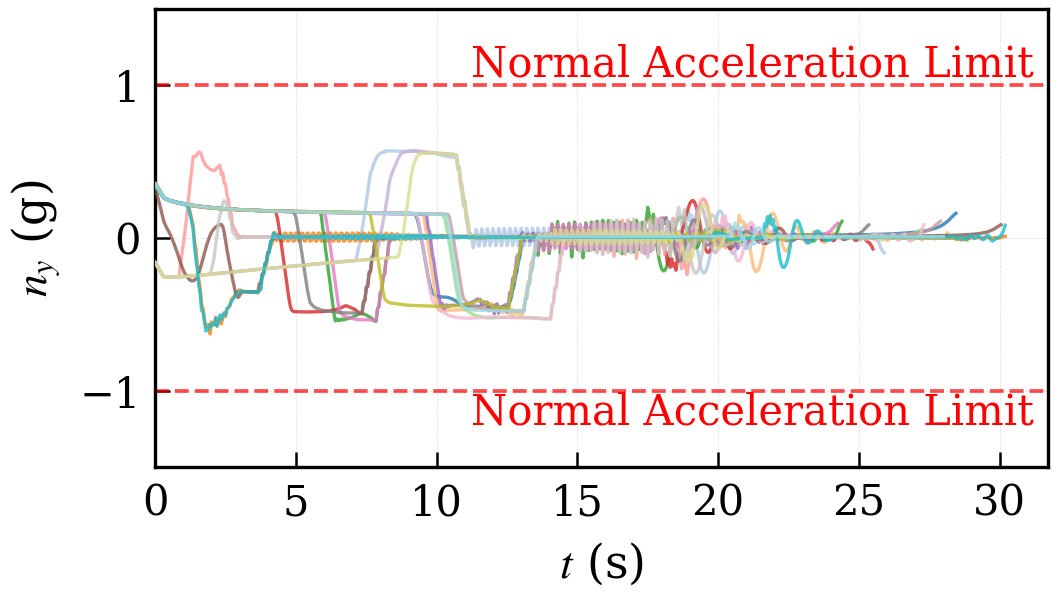
\includegraphics[width=3.0in]{mappo_nopn_ny.png}}
%DIFDELCMD < \hfil
%DIFDELCMD < \subfloat[Heading angle $\gamma_D$]{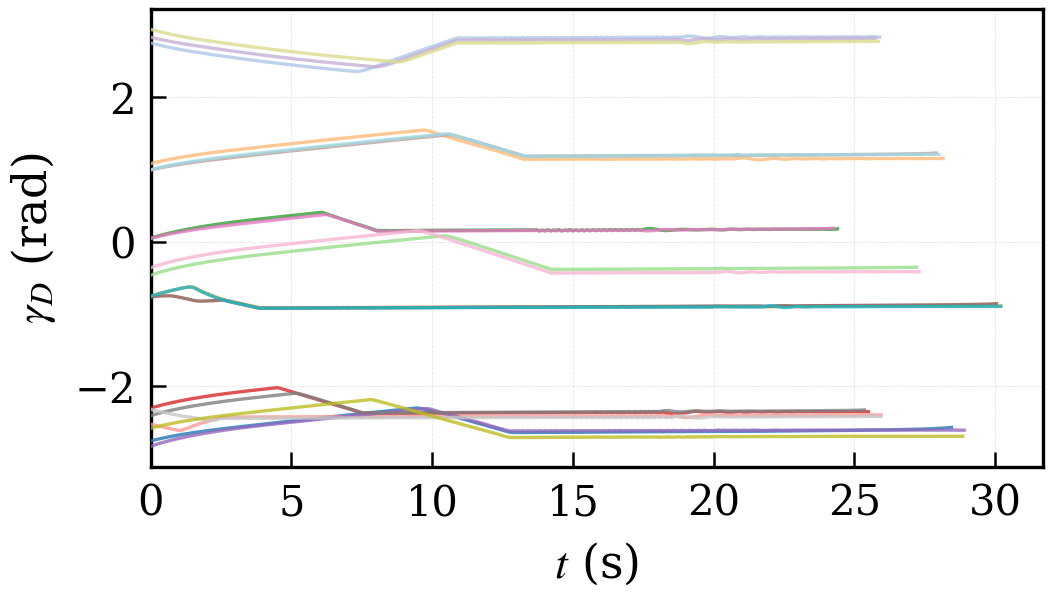
\includegraphics[width=3.0in]{mappo_nopn_heading.png}}
%DIFDELCMD < \hfil
%DIFDELCMD < \subfloat[Velocity $V_D$]{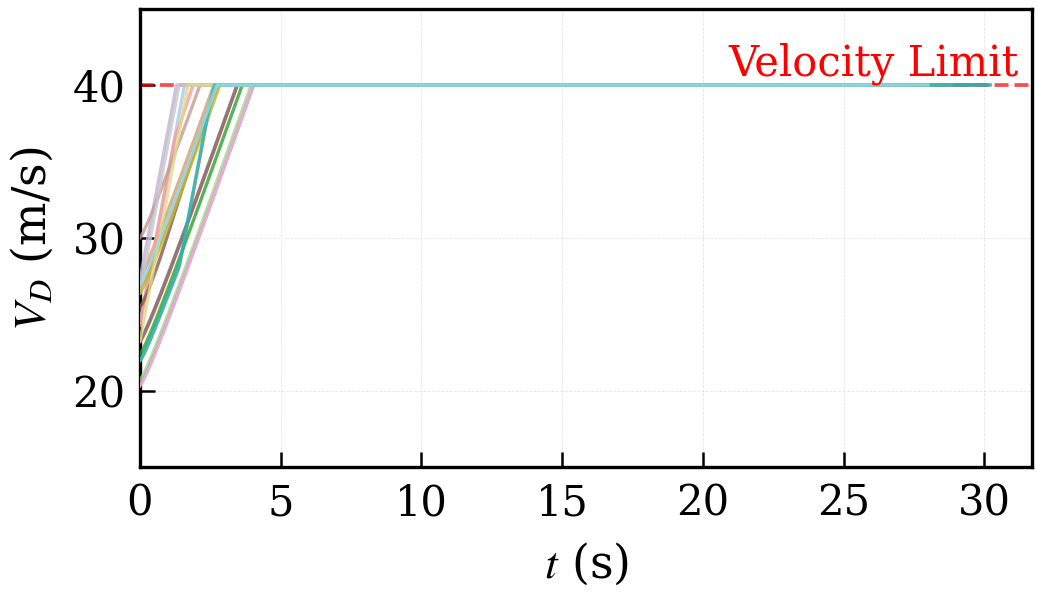
\includegraphics[width=3.0in]{mappo_nopn_velocity.png}}
%DIFDELCMD < \hfil
%DIFDELCMD < \subfloat[Axial acceleration $n_x$]{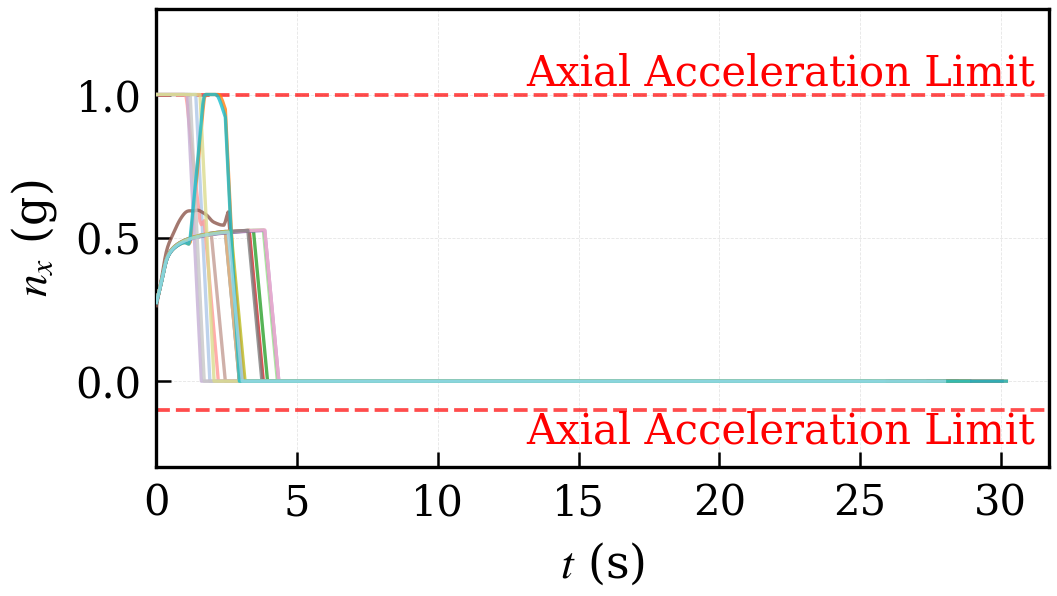
\includegraphics[width=3.0in]{mappo_nopn_nx.png}}
%DIFDELCMD < \vspace{0pt}
%DIFDELCMD < %%%
\DIFdelendFL \DIFaddbeginFL 
\includegraphics[width=3.2in]{../new_sim_fig/figures_v10/mappo/mappo_nopn_tgo.png}
\DIFaddendFL \caption{\DIFdelbeginFL \DIFdelFL{Kinematic and control effort }\DIFdelendFL \DIFaddbeginFL \DIFaddFL{Time-to-go ($t_{go}$) }\DIFaddendFL profiles of \DIFaddbeginFL \DIFaddFL{the defending swarm using }\DIFaddendFL ART-MAPPO \DIFdelbeginFL \DIFdelFL{for }\DIFdelendFL \DIFaddbeginFL \DIFaddFL{in }\DIFaddendFL Case~1.\DIFdelbeginFL \DIFdelFL{The algorithm successfully maximizes closing speed while strictly adhering to the $\pm1$\,g normal overload constraint.}\DIFdelendFL }
\DIFdelbeginFL %DIFDELCMD < \label{fig:case1_mappo_kine}
%DIFDELCMD < %%%
\DIFdelendFL \DIFaddbeginFL \label{fig:case1_mappo_tgo}
\DIFaddendFL \end{figure}

\DIFdelbegin \DIFdel{In stark contrast, the performance of the baseline PN guidance is presented in
Fig.~\ref{fig:case1_pn_traj} andFig.~\ref{fig:case1_pn_kine}. While PN eventually intercepts the targets (Fig.~\ref{fig:case1_pn_traj}), }\DIFdelend \DIFaddbegin \begin{figure}[!ht]
\centering

\includegraphics[width=3.0in]{../new_sim_fig/figures_v10/mappo/mappo_nopn_time_sync.png}
\caption{\DIFaddFL{Terminal arrival time differences $\Delta t$ within each ART-MAPPO interceptor group
in Case~1.}}
\label{fig:case1_mappo_sync}
\end{figure}

\emph{\DIFadd{2) PN baseline:}} \DIFadd{The capacity-matched PN reference is shown in
Figs.~\ref{fig:case1_pn_traj_3d} and~\ref{fig:case1_pn_traj_xy}. PN also completes the selected
engagement, but }\DIFaddend its purely reactive \DIFdelbegin \DIFdel{nature leads to a highly inefficient pursuit strategy. As clearly depicted in Fig.~\ref{fig:case1_pn_kine}(a), the normal acceleration ($n_y$) of PN drastically diverges, severely violating the $\pm1$\,g physical limit because the algorithm lacks predictive capability against evasive maneuvers, thus demanding excessive and
sudden control efforts in the terminal phase. In realistic flight conditions, such catastrophic actuator saturation would inevitably result in structural damage or loss of control, rendering the interception a failure. Consequently, the velocity decays significantly over time (Fig.~\ref{fig:case1_pn_kine}(c)), dragging out the interception duration}\DIFdelend \DIFaddbegin \DIFadd{commands produce visibly different spatial curvature and
control transients. The same command limits are imposed on both methods, so the comparison does
not attribute physically unavailable load authority to the baseline}\DIFaddend .

\begin{figure}[!ht]
\centering
\DIFdelbeginFL %DIFDELCMD < 
\includegraphics[width=3.2in]{pn_nopn_trajectory.png}
%DIFDELCMD < %%%
\DIFdelendFL \DIFaddbeginFL 
\includegraphics[width=3.15in]{../new_sim_fig/figures_v10/pn/pn_nopn_trajectory_3d.png}
\DIFaddendFL \caption{\DIFdelbeginFL \DIFdelFL{Engagement }\DIFdelendFL \DIFaddbeginFL \DIFaddFL{Three-dimensional engagement }\DIFaddendFL trajectories of the defending swarm using the PN
baseline in Case~1.}
\DIFdelbeginFL %DIFDELCMD < \label{fig:case1_pn_traj}
%DIFDELCMD < %%%
\DIFdelendFL \DIFaddbeginFL \label{fig:case1_pn_traj_3d}
\DIFaddendFL \end{figure}

\begin{figure}[!ht]
\centering
\DIFdelbeginFL %DIFDELCMD < 
\includegraphics[width=3.0in]{standalone_duav_legend.png}
%DIFDELCMD < \subfloat[Normal acceleration $n_y$]{
\includegraphics[width=3.0in]{pn_nopn_ny.png}}
%DIFDELCMD < \hfil
%DIFDELCMD < \subfloat[Heading angle $\gamma_D$]{
\includegraphics[width=3.0in]{pn_nopn_heading.png}}
%DIFDELCMD < \hfil
%DIFDELCMD < \subfloat[Velocity $V_D$]{
\includegraphics[width=3.0in]{pn_nopn_velocity.png}}
%DIFDELCMD < \hfil
%DIFDELCMD < \subfloat[Axial acceleration $n_x$]{
\includegraphics[width=3.0in]{pn_nopn_nx.png}}
%DIFDELCMD < \vspace{0pt}
%DIFDELCMD < %%%
\DIFdelendFL \DIFaddbeginFL 
\includegraphics[width=3.15in]{../new_sim_fig/figures_v10/pn/pn_nopn_trajectory.png}
\DIFaddendFL \caption{\DIFdelbeginFL \DIFdelFL{Kinematic }\DIFdelendFL \DIFaddbeginFL \DIFaddFL{Horizontal projection of the PN engagement trajectories in Case~1.}}
\label{fig:case1_pn_traj_xy}
\end{figure}

\DIFadd{Figures~\ref{fig:case1_pn_yaw}--\ref{fig:case1_pn_axial} give the corresponding yaw-plane,
pitch-plane, and axial responses. The PN commands are clipped to $n_x\in[-0.1,1]$ }\DIFaddend and
\DIFdelbegin \DIFdel{control effort profiles }\DIFdelend \DIFaddbegin \DIFadd{$n_y,n_z\in[-1,1]$, and the command histories show more direct use of the available bounds.
The pitch response remains finite and the speed histories remain within the common vehicle
envelope, providing a physically matched three-dimensional reference.
}

\begin{figure}[!ht]
\centering

\includegraphics[width=3.1in]{../new_sim_fig/figures_v10/pn/standalone_duav_legend.png}\\[-2pt]
\subfloat[Normal load $n_y$]{
\includegraphics[width=3.2in]{../new_sim_fig/figures_v10/pn/pn_nopn_ny.png}}\\[-2pt]
\subfloat[Heading $\gamma_D$]{
\includegraphics[width=3.2in]{../new_sim_fig/figures_v10/pn/pn_nopn_heading.png}}
\caption{\DIFaddFL{Yaw-plane command and response }\DIFaddendFL of the \DIFaddbeginFL \DIFaddFL{capacity-matched }\DIFaddendFL PN baseline \DIFdelbeginFL \DIFdelFL{for }\DIFdelendFL \DIFaddbeginFL \DIFaddFL{in }\DIFaddendFL Case~\DIFdelbeginFL \DIFdelFL{1, illustrating severe terminal actuator saturation ($n_y$ exceeding $\pm1$\,g limits).}\DIFdelendFL \DIFaddbeginFL \DIFaddFL{1.}\DIFaddendFL }
\DIFdelbeginFL %DIFDELCMD < \label{fig:case1_pn_kine}
%DIFDELCMD < %%%
\DIFdelendFL \DIFaddbeginFL \label{fig:case1_pn_yaw}
\DIFaddendFL \end{figure}

\DIFdelbegin \DIFdel{Beyond individual interception capabilities, a core requirement of swarm defense is the execution of a simultaneous saturation strike to prevent the targets from defeating the interceptors piecemeal. This vital temporal coordination is dynamically achieved during the flight,
as evidenced by the time-to-go ($t_{go}$) profiles in Fig.~\ref{fig:case1_mappo_tgo}. The }\DIFdelend \DIFaddbegin \begin{figure}[!ht]
\centering

\includegraphics[width=3.1in]{../new_sim_fig/figures_v10/pn/standalone_duav_legend.png}\\[-2pt]
\subfloat[Vertical load $n_z$]{
\includegraphics[width=3.2in]{../new_sim_fig/figures_v10/pn/pn_nopn_nz.png}}\\[-2pt]
\subfloat[Pitch $\theta_D$]{
\includegraphics[width=3.2in]{../new_sim_fig/figures_v10/pn/pn_nopn_pitch.png}}
\caption{\DIFaddFL{Pitch-plane command and response of the capacity-matched PN baseline in Case~1.}}
\label{fig:case1_pn_pitch}
\end{figure}

\begin{figure}[!ht]
\centering

\includegraphics[width=3.1in]{../new_sim_fig/figures_v10/pn/standalone_duav_legend.png}\\[-2pt]
\subfloat[Axial load $n_x$]{
\includegraphics[width=3.2in]{../new_sim_fig/figures_v10/pn/pn_nopn_nx.png}}\\[-2pt]
\subfloat[Velocity $V_D$]{
\includegraphics[width=3.2in]{../new_sim_fig/figures_v10/pn/pn_nopn_velocity.png}}
\caption{\DIFaddFL{Axial command and speed response of the capacity-matched PN baseline in Case~1.}}
\label{fig:case1_pn_axial}
\end{figure}

\DIFadd{The PN }\DIFaddend $t_{go}$ \DIFdelbegin \DIFdel{curves of interceptors assigned to the same target rapidly converge as the engagement progresses. This explicitly demonstrates that ART-MAPPO actively shapes the velocity distribution of the swarm to synchronize the remaining flight times long before the actual impact}\DIFdelend \DIFaddbegin \DIFadd{histories also converge in this selected run, as shown in
Fig.~\ref{fig:case1_pn_tgo}. Its maximum terminal group spread is 0.40\,s
(Fig.~\ref{fig:case1_pn_sync}), compared with 0.25\,s for ART-MAPPO. Both satisfy the 0.5-s
criterion, while the learned policy gives the tighter representative Case~1 synchronization}\DIFaddend .

\begin{figure}[!ht]
\centering
\DIFdelbeginFL %DIFDELCMD < 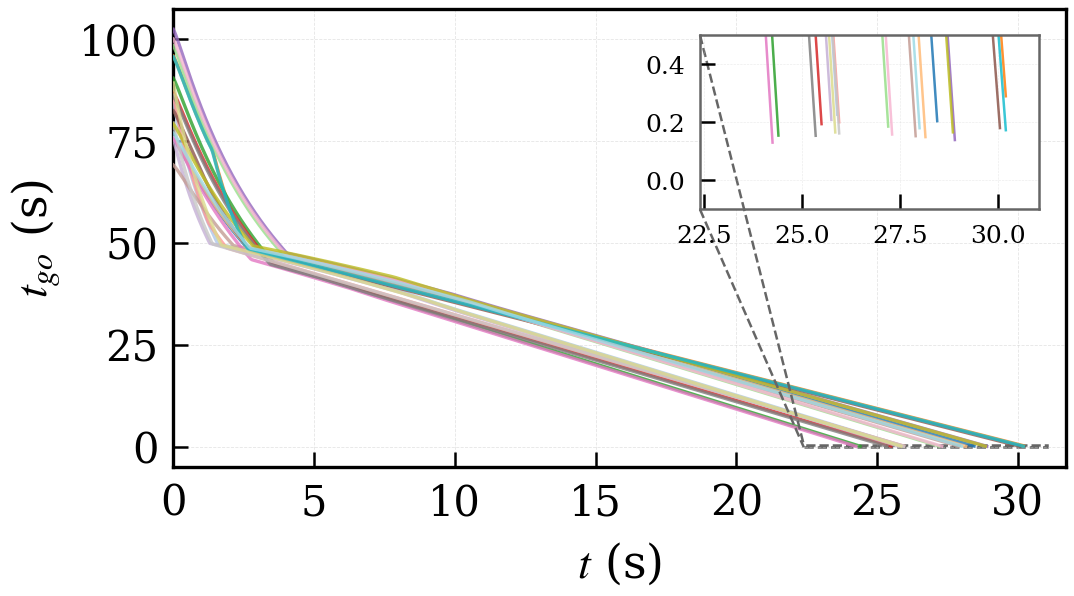
\includegraphics[width=3.2in]{mappo_nopn_tgo.png}
%DIFDELCMD < %%%
\DIFdelendFL \DIFaddbeginFL 
\includegraphics[width=3.2in]{../new_sim_fig/figures_v10/pn/pn_nopn_tgo.png}
\DIFaddendFL \caption{Time-to-go ($t_{go}$) profiles of the defending swarm using \DIFdelbeginFL \DIFdelFL{ART-MAPPO }\DIFdelendFL \DIFaddbeginFL \DIFaddFL{the PN baseline }\DIFaddendFL in
Case~1.\DIFdelbeginFL \DIFdelFL{Interceptors assigned to the same target actively synchronize their remaining flight times to guarantee a simultaneous saturation strike.}\DIFdelendFL }
\DIFdelbeginFL %DIFDELCMD < \label{fig:case1_mappo_tgo}
%DIFDELCMD < %%%
\DIFdelendFL \DIFaddbeginFL \label{fig:case1_pn_tgo}
\DIFaddendFL \end{figure}

\DIFdelbegin \DIFdel{Consequently, Fig.~\ref{fig:case1_time_sync} explicitly validates the ultimate temporal coordination capability by displaying the terminal arrival time difference ($\Delta t$) among the interceptors assigned to each respective target group. The maximum $\Delta t$ across all eight coordinated groups is remarkably tight, bounded to merely 0.45\,s. This quantitatively proves that the proposed framework perfectly bridges the target assignment and the trust-modulated exploration mechanisms, ensuring a strictly temporally coordinated saturation strike against the swarm threat.
}%DIFDELCMD < 

%DIFDELCMD < %%%
\DIFdelend \begin{figure}[!ht]
\centering
\DIFdelbeginFL %DIFDELCMD < 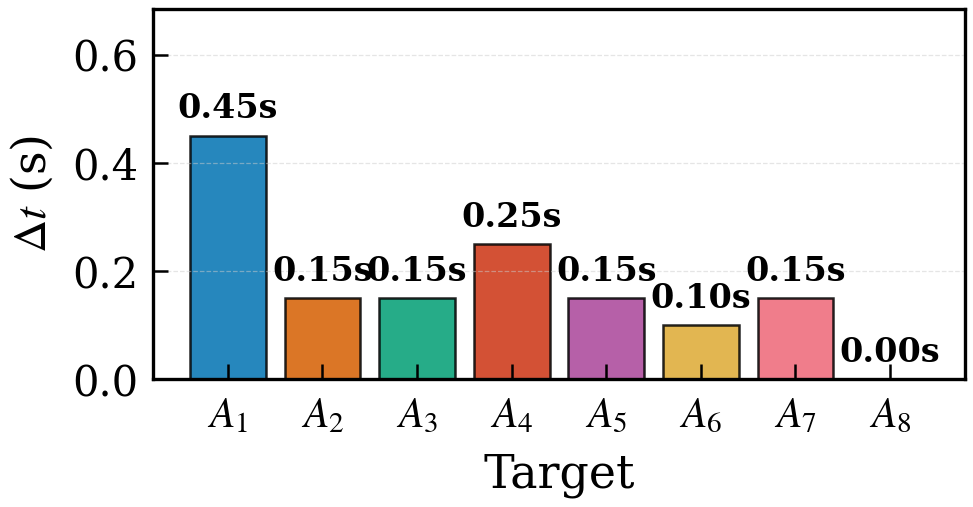
\includegraphics[width=3.0in]{mappo_success_nopn_time_sync.png}
%DIFDELCMD < \caption{%%%
\DIFdelFL{Terminal arrival time differences $\Delta t$ within each coordinated interceptor group under ART-MAPPO. The near-zero $\Delta t$ values explicitly validate the successful execution of temporally synchronized saturation strikes.}%DIFDELCMD < \MBLOCKRIGHTBRACE
%DIFDELCMD < \label{fig:case1_time_sync}
%DIFDELCMD < %%%
\DIFdelendFL \DIFaddbeginFL 
\includegraphics[width=3.0in]{../new_sim_fig/figures_v10/pn/pn_nopn_time_sync.png}
\caption{\DIFaddFL{Terminal arrival time differences $\Delta t$ within each PN interceptor group in
Case~1.}}
\label{fig:case1_pn_sync}
\DIFaddendFL \end{figure}
\DIFaddbegin \FloatBarrier
\DIFaddend 

\subsubsection{Case~2: Interception against Continuous Weaving Targets}

\DIFdelbegin \DIFdel{This scenario evaluates the robustness of the proposed framework against the }\DIFdelend \DIFaddbegin \DIFadd{Case~2 uses a }\DIFaddend sinusoidal penetration maneuver~\cite{Zarchan1995969}\DIFdelbegin \DIFdel{, which represents a highly agile and continuous weaving threat. Such maneuvers induce high-frequency oscillations in the line-of-sight (LOS ) rate, severely challenging both the guidance stability and the temporal coordination of the defending swarm}\DIFdelend \DIFaddbegin \DIFadd{. Its continuous horizontal
and vertical LOS variation provides a more persistent disturbance than the Case~1 transition
and tests whether group timing can be maintained while all three command channels respond}\DIFaddend .

\DIFdelbegin \DIFdel{The 2D engagement trajectories of the ART-MAPPO defending swarm are illustrated }\DIFdelend \DIFaddbegin \emph{\DIFadd{1) ART-MAPPO:}} \DIFadd{The three-dimensional paths }\DIFaddend in
Fig.~\DIFdelbegin \DIFdel{\ref{fig:case2_mappo_traj}. Despite the continuous lateral oscillations of the $A_{\text{UAV}}$, ART-MAPPO explicitly predicts and accommodates the target's weaving motion. The defending swarm maintains all eight coordinated combat units and successfully intercepts every target with smooth pursuit curves}\DIFdelend \DIFaddbegin \DIFadd{\ref{fig:case2_mappo_traj_3d} show that all eight groups maintain spatial closure against
the weaving targets. The horizontal projection in Fig.~\ref{fig:case2_mappo_traj_xy} exposes
the lateral curvature without hiding the altitude evolution shown in the 3-D view}\DIFaddend .

\begin{figure}[!ht]
\centering
\DIFdelbeginFL %DIFDELCMD < 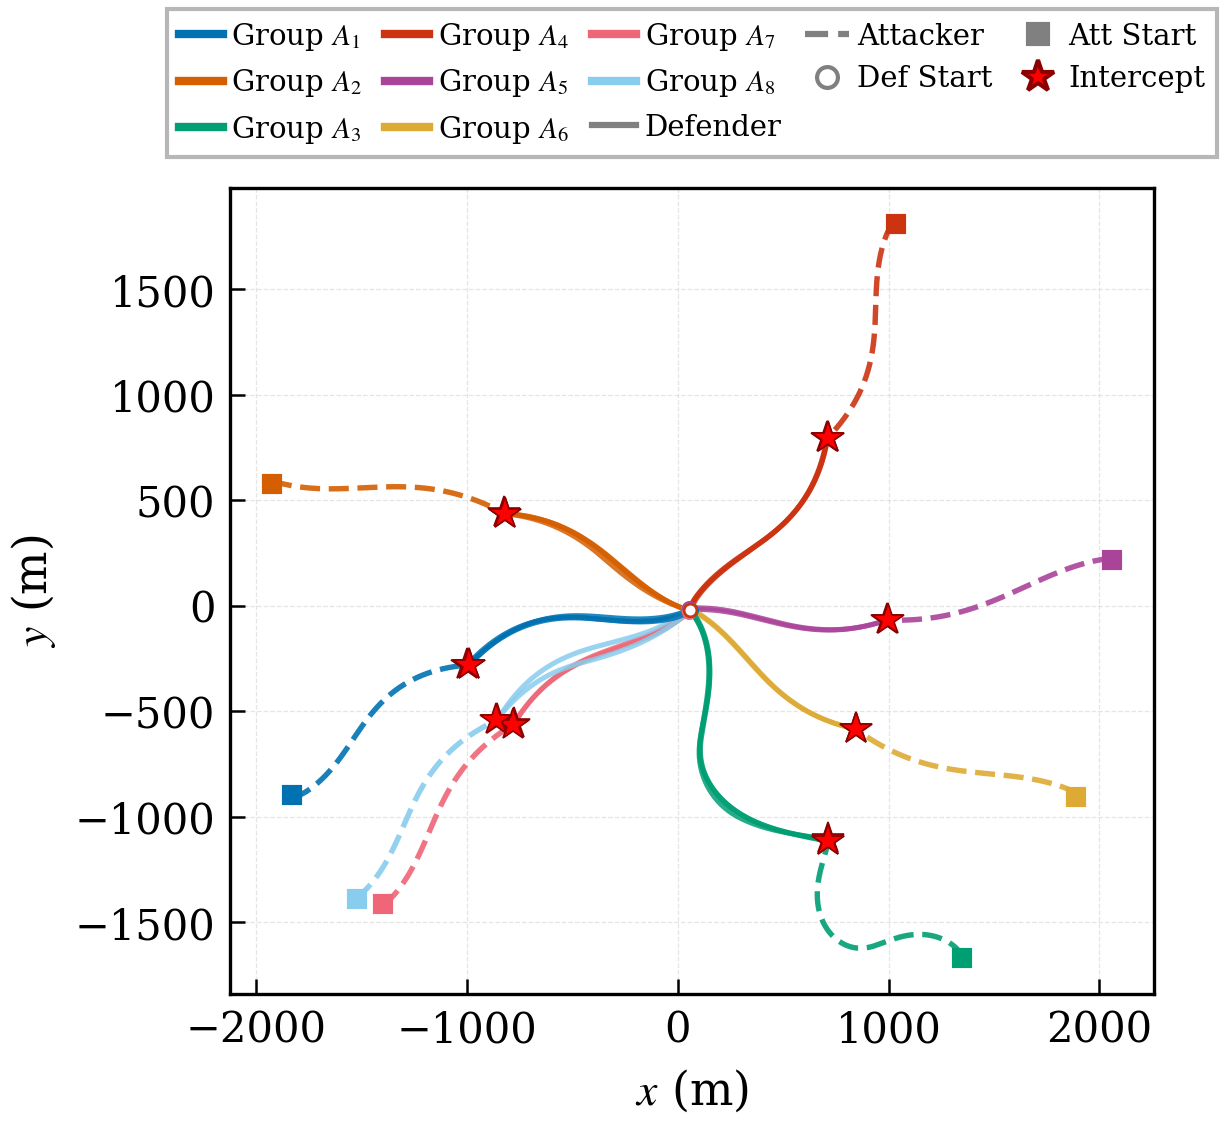
\includegraphics[width=3.2in]{mappo_sin_trajectory.png}
%DIFDELCMD < %%%
\DIFdelendFL \DIFaddbeginFL 
\includegraphics[width=3.15in]{../new_sim_fig/figures_v10/mappo/mappo_sin_trajectory_3d.png}
\DIFaddendFL \caption{\DIFdelbeginFL \DIFdelFL{Engagement trajectories of the defending swarm using }\DIFdelendFL \DIFaddbeginFL \DIFaddFL{Three-dimensional }\DIFaddendFL ART-MAPPO \DIFaddbeginFL \DIFaddFL{engagement trajectories }\DIFaddendFL against continuous weaving
targets \DIFdelbeginFL \DIFdelFL{(}\DIFdelendFL \DIFaddbeginFL \DIFaddFL{in }\DIFaddendFL Case~\DIFdelbeginFL \DIFdelFL{2).}\DIFdelendFL \DIFaddbeginFL \DIFaddFL{2.}\DIFaddendFL }
\DIFdelbeginFL %DIFDELCMD < \label{fig:case2_mappo_traj}
%DIFDELCMD < %%%
\DIFdelendFL \DIFaddbeginFL \label{fig:case2_mappo_traj_3d}
\DIFaddendFL \end{figure}

\DIFdelbegin \DIFdel{The underlying kinematic and control mechanisms of ART-MAPPO are further detailed in Fig.~\ref{fig:case2_mappo_kine}. The most significant advantage is observed in the normal acceleration profile ($n_y$) shown in Fig.~\ref{fig:case2_mappo_kine}(a). To counter the weaving target}\DIFdelend \DIFaddbegin \begin{figure}[!ht]
\centering

\includegraphics[width=3.15in]{../new_sim_fig/figures_v10/mappo/mappo_sin_trajectory.png}
\caption{\DIFaddFL{Horizontal projection of the ART-MAPPO engagement trajectories in Case~2.}}
\label{fig:case2_mappo_traj_xy}
\end{figure}

\DIFadd{As shown in Figs.~\ref{fig:case2_mappo_yaw}--\ref{fig:case2_mappo_axial}}\DIFaddend , ART-MAPPO \DIFdelbegin \DIFdel{generates an intelligent, adaptive oscillatory }\DIFdelend \DIFaddbegin \DIFadd{adapts
}\DIFaddend $n_y$ \DIFdelbegin \DIFdel{command that perfectly tracks the target's maneuvering frequency. Most importantly, it achieves this dynamic tracking while strictly remaining within the safe aerodynamic envelope ($\pm 1$\,g), completely averting terminal saturation.
Furthermore, it smoothly adjusts its heading angle (Fig.~\ref{fig:case2_mappo_kine}(b)). Similar to Case~1, ART-MAPPO aggressively leverages its axial acceleration ($n_x$) to maximize approach velocity, as demonstrated in the velocity and axial acceleration profiles (Fig.~\ref{fig:case2_mappo_kine}(c) and (d))}\DIFdelend \DIFaddbegin \DIFadd{to the continuous lateral disturbance while using $n_z$ to regulate vertical closure.
The heading and pitch histories
remain smooth relative to the command variations, and all load channels remain inside the
prescribed envelope. The axial command raises or preserves closing speed without eliminating
the control authority required in the yaw and pitch planes}\DIFaddend .

\begin{figure}[!ht]
\centering
\DIFdelbeginFL %DIFDELCMD < 
\includegraphics[width=3.0in]{standalone_duav_legend.png}
%DIFDELCMD < \subfloat[Normal acceleration $n_y$]{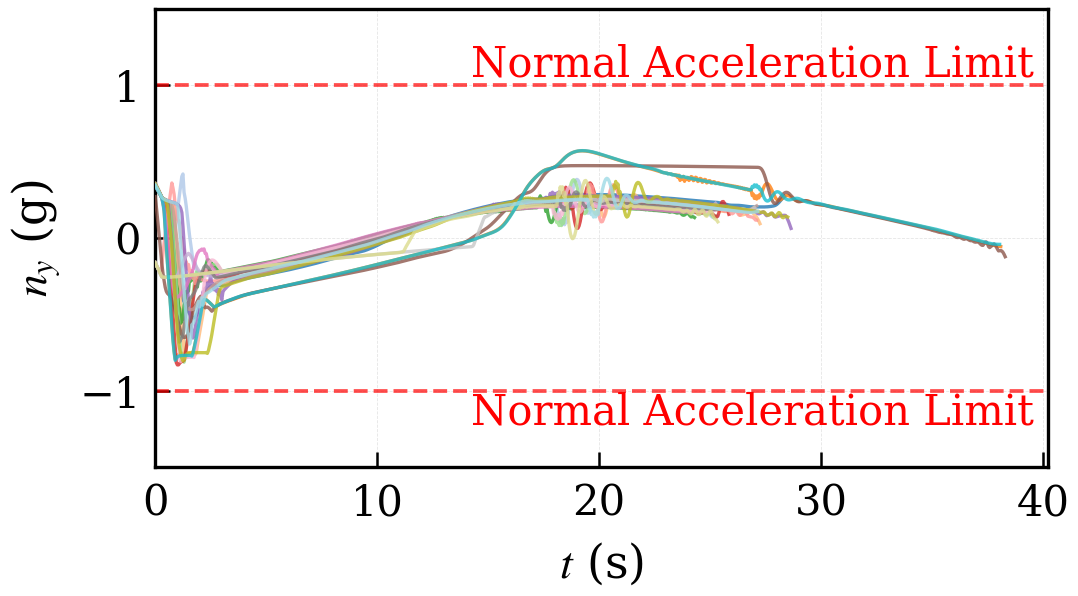
\includegraphics[width=3.0in]{mappo_sin_ny.png}}
%DIFDELCMD < \hfil
%DIFDELCMD < \subfloat[Heading angle $\gamma_D$]{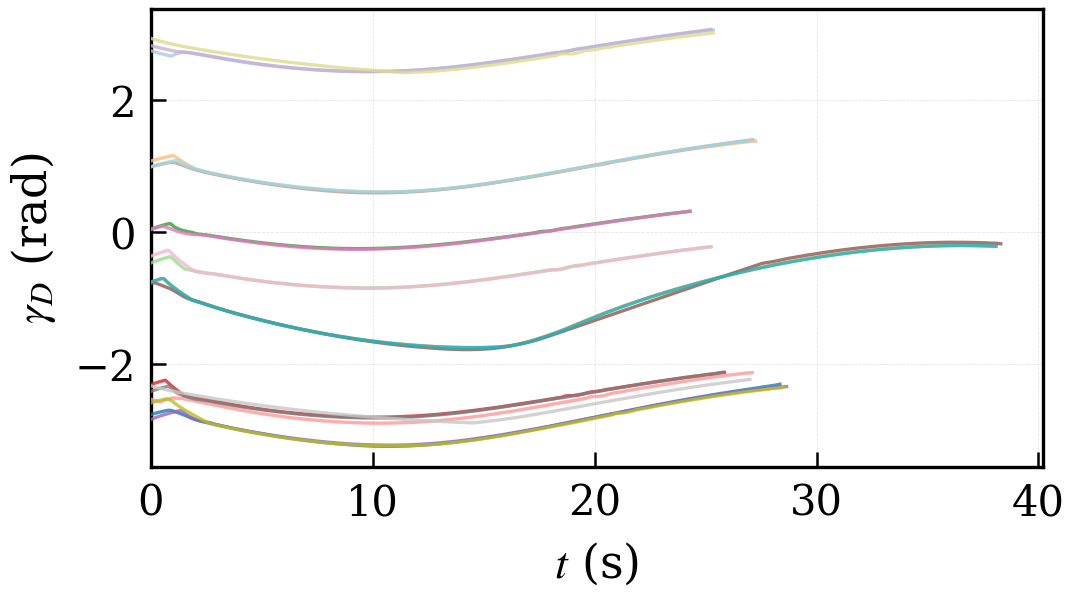
\includegraphics[width=3.0in]{mappo_sin_heading.png}}
%DIFDELCMD < \hfil
%DIFDELCMD < \subfloat[Velocity $V_D$]{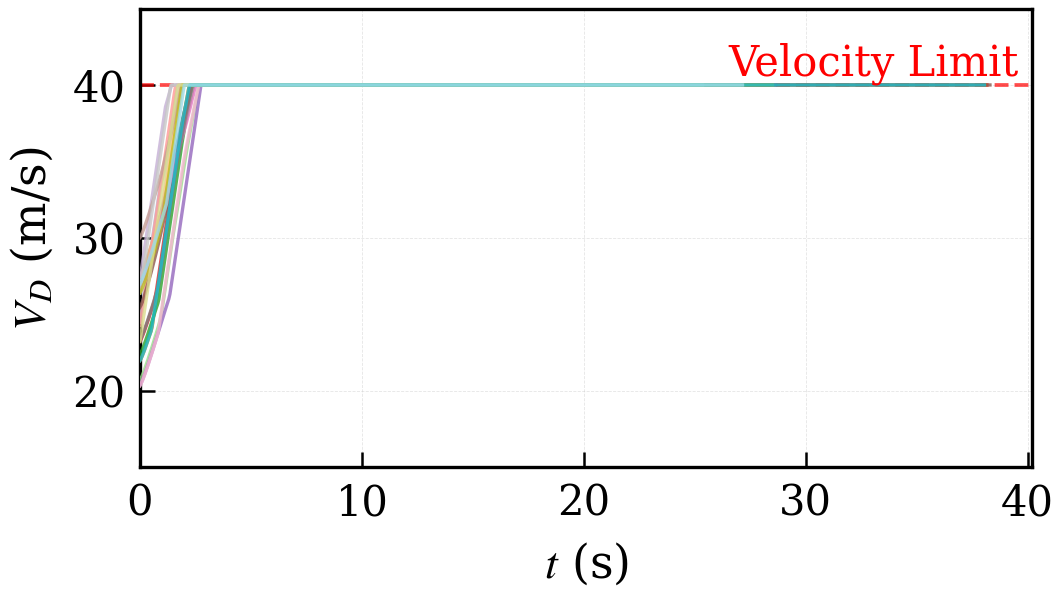
\includegraphics[width=3.0in]{mappo_sin_velocity.png}}
%DIFDELCMD < \hfil
%DIFDELCMD < \subfloat[Axial acceleration $n_x$]{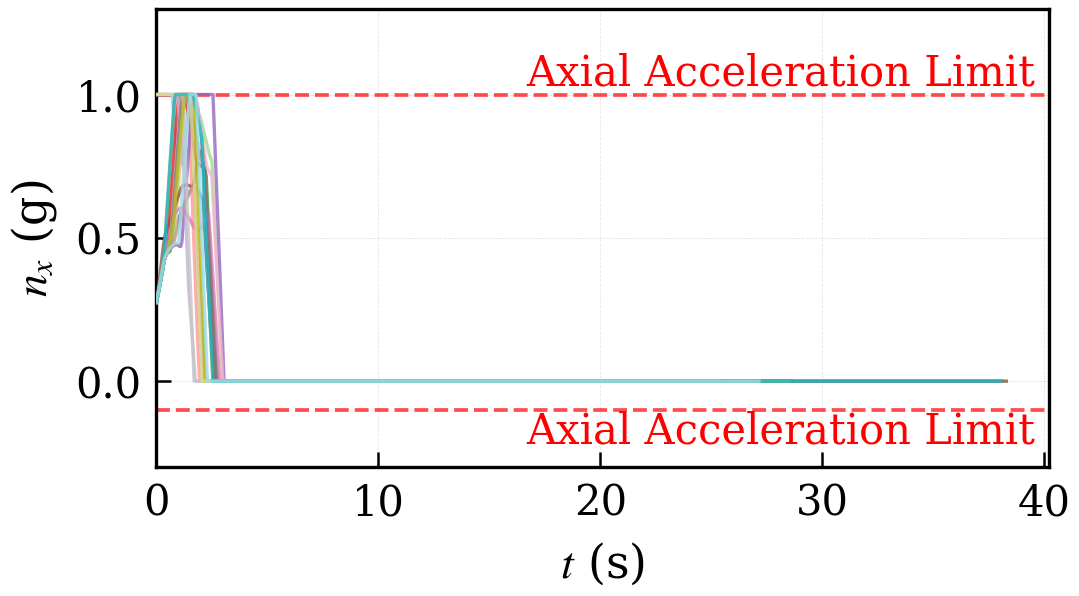
\includegraphics[width=3.0in]{mappo_sin_nx.png}}
%DIFDELCMD < \vspace{0pt}
%DIFDELCMD < %%%
\DIFdelendFL \DIFaddbeginFL 
\includegraphics[width=3.1in]{../new_sim_fig/figures_v10/mappo/standalone_duav_legend.png}\\[-2pt]
\subfloat[Normal load $n_y$]{
\includegraphics[width=3.2in]{../new_sim_fig/figures_v10/mappo/mappo_sin_ny.png}}\\[-2pt]
\subfloat[Heading $\gamma_D$]{
\includegraphics[width=3.2in]{../new_sim_fig/figures_v10/mappo/mappo_sin_heading.png}}
\DIFaddendFL \caption{\DIFdelbeginFL \DIFdelFL{Kinematic }\DIFdelendFL \DIFaddbeginFL \DIFaddFL{Yaw-plane command }\DIFaddendFL and \DIFdelbeginFL \DIFdelFL{control effort profiles }\DIFdelendFL \DIFaddbeginFL \DIFaddFL{response }\DIFaddendFL of ART-MAPPO \DIFdelbeginFL \DIFdelFL{for }\DIFdelendFL \DIFaddbeginFL \DIFaddFL{in }\DIFaddendFL Case~2.\DIFdelbeginFL \DIFdelFL{The policy dynamically outputs adaptive oscillatory normal commands ($n_y$) to track the weaving target without violating the $\pm1$\,g limit.}\DIFdelendFL }
\DIFdelbeginFL %DIFDELCMD < \label{fig:case2_mappo_kine}
%DIFDELCMD < %%%
\DIFdelendFL \DIFaddbeginFL \label{fig:case2_mappo_yaw}
\DIFaddendFL \end{figure}

\DIFdelbegin \DIFdel{Conversely, the PN baseline completely fails to handle the high-frequency dynamic engagement geometry. The reactive nature of PN results in phase-lagged trajectories that struggle to close the distance }\DIFdelend \DIFaddbegin \begin{figure}[!ht]
\centering

\includegraphics[width=3.1in]{../new_sim_fig/figures_v10/mappo/standalone_duav_legend.png}\\[-2pt]
\subfloat[Vertical load $n_z$]{
\includegraphics[width=3.2in]{../new_sim_fig/figures_v10/mappo/mappo_sin_nz.png}}\\[-2pt]
\subfloat[Pitch $\theta_D$]{
\includegraphics[width=3.2in]{../new_sim_fig/figures_v10/mappo/mappo_sin_pitch.png}}
\caption{\DIFaddFL{Pitch-plane command and response of ART-MAPPO in Case~2.}}
\label{fig:case2_mappo_pitch}
\end{figure}

\begin{figure}[!ht]
\centering

\includegraphics[width=3.1in]{../new_sim_fig/figures_v10/mappo/standalone_duav_legend.png}\\[-2pt]
\subfloat[Axial load $n_x$]{
\includegraphics[width=3.2in]{../new_sim_fig/figures_v10/mappo/mappo_sin_nx.png}}\\[-2pt]
\subfloat[Velocity $V_D$]{
\includegraphics[width=3.2in]{../new_sim_fig/figures_v10/mappo/mappo_sin_velocity.png}}
\caption{\DIFaddFL{Axial command and speed response of ART-MAPPO in Case~2.}}
\label{fig:case2_mappo_axial}
\end{figure}

\DIFadd{Despite the continuous LOS disturbance, the ART-MAPPO $t_{go}$ curves converge within their
assigned groups }\DIFaddend (Fig.~\DIFdelbegin \DIFdel{\ref{fig:case2_pn_traj}). As revealed in the control profiles (Fig.~\ref{fig:case2_pn_kine}), the PN guidance law suffers from catastrophic actuator saturation during the terminal phase. Specifically, the normal commands ($n_y$) frequently breach the $\pm 1$}\DIFdelend \DIFaddbegin \DIFadd{\ref{fig:case2_mappo_tgo}). The largest terminal arrival-time difference
is 0.30}\DIFaddend \,\DIFdelbegin \DIFdel{g limit (}\DIFdelend \DIFaddbegin \DIFadd{s in }\DIFaddend Fig.~\DIFdelbegin \DIFdel{\ref{fig:case2_pn_kine}(a)), which would severely compromise flight safety and render the interception a failure in real-world applications}\DIFdelend \DIFaddbegin \DIFadd{\ref{fig:case2_mappo_sync}, demonstrating that the timing objective remains
active in the three-dimensional engagement}\DIFaddend .

\begin{figure}[!ht]
\centering
\DIFdelbeginFL %DIFDELCMD < 
\includegraphics[width=3.2in]{pn_sin_trajectory.png}
%DIFDELCMD < %%%
\DIFdelendFL \DIFaddbeginFL 
\includegraphics[width=3.2in]{../new_sim_fig/figures_v10/mappo/mappo_sin_tgo.png}
\DIFaddendFL \caption{\DIFdelbeginFL \DIFdelFL{Engagement trajectories }\DIFdelendFL \DIFaddbeginFL \DIFaddFL{Time-to-go ($t_{go}$) profiles }\DIFaddendFL of the defending swarm using \DIFdelbeginFL \DIFdelFL{the PN baseline }\DIFdelendFL \DIFaddbeginFL \DIFaddFL{ART-MAPPO }\DIFaddendFL in Case~2.}
\DIFdelbeginFL %DIFDELCMD < \label{fig:case2_pn_traj}
%DIFDELCMD < %%%
\DIFdelendFL \DIFaddbeginFL \label{fig:case2_mappo_tgo}
\DIFaddendFL \end{figure}

\begin{figure}[!ht]
\centering
\DIFdelbeginFL %DIFDELCMD < 
\includegraphics[width=3.0in]{standalone_duav_legend.png}
%DIFDELCMD < \subfloat[Normal acceleration $n_y$]{
\includegraphics[width=3.0in]{pn_sin_ny.png}}
%DIFDELCMD < \hfil
%DIFDELCMD < \subfloat[Heading angle $\gamma_D$]{
\includegraphics[width=3.0in]{pn_sin_heading.png}}
%DIFDELCMD < \hfil
%DIFDELCMD < \subfloat[Velocity $V_D$]{
\includegraphics[width=3.0in]{pn_sin_velocity.png}}
%DIFDELCMD < \hfil
%DIFDELCMD < \subfloat[Axial acceleration $n_x$]{
\includegraphics[width=3.0in]{pn_sin_nx.png}}
%DIFDELCMD < \vspace{0pt}
%DIFDELCMD < %%%
\DIFdelendFL \DIFaddbeginFL 
\includegraphics[width=3.0in]{../new_sim_fig/figures_v10/mappo/mappo_sin_time_sync.png}
\DIFaddendFL \caption{\DIFdelbeginFL \DIFdelFL{Kinematic }\DIFdelendFL \DIFaddbeginFL \DIFaddFL{Terminal arrival time differences $\Delta t$ within each ART-MAPPO interceptor group
in Case~2.}}
\label{fig:case2_mappo_sync}
\end{figure}

\emph{\DIFadd{2) PN baseline:}} \DIFadd{Figures~\ref{fig:case2_pn_traj_3d}
and~\ref{fig:case2_pn_traj_xy} show that the constrained PN baseline also reaches all assigned
targets in the selected Case~2 engagement. The spatial paths exhibit the reactive response to
the continuously varying LOS, while the plan view and 3-D view together distinguish lateral
curvature from vertical closure.
}

\begin{figure}[!ht]
\centering

\includegraphics[width=3.15in]{../new_sim_fig/figures_v10/pn/pn_sin_trajectory_3d.png}
\caption{\DIFaddFL{Three-dimensional engagement trajectories of the defending swarm using the PN
baseline in Case~2.}}
\label{fig:case2_pn_traj_3d}
\end{figure}

\begin{figure}[!ht]
\centering

\includegraphics[width=3.15in]{../new_sim_fig/figures_v10/pn/pn_sin_trajectory.png}
\caption{\DIFaddFL{Horizontal projection of the PN engagement trajectories in Case~2.}}
\label{fig:case2_pn_traj_xy}
\end{figure}

\DIFadd{The PN profiles in Figs.~\ref{fig:case2_pn_yaw}--\ref{fig:case2_pn_axial} show sustained
reactive changes in the horizontal channel together with the vertical and axial responses.
Since all commands are
clipped to the same envelope as ART-MAPPO, excursions that reach the plotted $\pm1$ lines
represent saturation of available authority rather than an unrealizable command.
}

\begin{figure}[!ht]
\centering

\includegraphics[width=3.1in]{../new_sim_fig/figures_v10/pn/standalone_duav_legend.png}\\[-2pt]
\subfloat[Normal load $n_y$]{
\includegraphics[width=3.2in]{../new_sim_fig/figures_v10/pn/pn_sin_ny.png}}\\[-2pt]
\subfloat[Heading $\gamma_D$]{
\includegraphics[width=3.2in]{../new_sim_fig/figures_v10/pn/pn_sin_heading.png}}
\caption{\DIFaddFL{Yaw-plane command }\DIFaddendFL and \DIFdelbeginFL \DIFdelFL{control effort profiles }\DIFdelendFL \DIFaddbeginFL \DIFaddFL{response }\DIFaddendFL of the \DIFaddbeginFL \DIFaddFL{capacity-matched }\DIFaddendFL PN baseline \DIFdelbeginFL \DIFdelFL{for }\DIFdelendFL \DIFaddbeginFL \DIFaddFL{in }\DIFaddendFL Case~\DIFdelbeginFL \DIFdelFL{2, highlighting catastrophic terminal actuator saturation ($n_y$ significantly exceeding limits).}\DIFdelendFL \DIFaddbeginFL \DIFaddFL{2.}\DIFaddendFL }
\DIFdelbeginFL %DIFDELCMD < \label{fig:case2_pn_kine}
%DIFDELCMD < %%%
\DIFdelendFL \DIFaddbeginFL \label{fig:case2_pn_yaw}
\DIFaddendFL \end{figure}

\DIFdelbegin \DIFdel{The continuous maneuvering of the targets also disrupts conventional coordination mechanisms. However, this vital temporal synchronization is dynamically sustained by ART-MAPPO during the flight, as evidenced by the }\DIFdelend \DIFaddbegin \begin{figure}[!ht]
\centering

\includegraphics[width=3.1in]{../new_sim_fig/figures_v10/pn/standalone_duav_legend.png}\\[-2pt]
\subfloat[Vertical load $n_z$]{
\includegraphics[width=3.2in]{../new_sim_fig/figures_v10/pn/pn_sin_nz.png}}\\[-2pt]
\subfloat[Pitch $\theta_D$]{
\includegraphics[width=3.2in]{../new_sim_fig/figures_v10/pn/pn_sin_pitch.png}}
\caption{\DIFaddFL{Pitch-plane command and response of the capacity-matched PN baseline in Case~2.}}
\label{fig:case2_pn_pitch}
\end{figure}

\begin{figure}[!ht]
\centering

\includegraphics[width=3.1in]{../new_sim_fig/figures_v10/pn/standalone_duav_legend.png}\\[-2pt]
\subfloat[Axial load $n_x$]{
\includegraphics[width=3.2in]{../new_sim_fig/figures_v10/pn/pn_sin_nx.png}}\\[-2pt]
\subfloat[Velocity $V_D$]{
\includegraphics[width=3.2in]{../new_sim_fig/figures_v10/pn/pn_sin_velocity.png}}
\caption{\DIFaddFL{Axial command and speed response of the capacity-matched PN baseline in Case~2.}}
\label{fig:case2_pn_axial}
\end{figure}

\DIFadd{Figure~\ref{fig:case2_pn_tgo} shows that the selected PN engagement also achieves groupwise
}\DIFaddend time-to-go \DIFdelbegin \DIFdel{($t_{go}$) profiles in Fig.~\ref{fig:case2_mappo_tgo}. Even against severe LOS oscillations, the $t_{go}$ curves of interceptors assigned to the same target smoothly converge. This demonstrates that the algorithm continuously and intelligently adapts the swarm's velocity distribution to lock in synchronized impact times, despite the highly dynamic nature of the weaving threats}\DIFdelend \DIFaddbegin \DIFadd{convergence. Its maximum arrival spread is 0.35\,s
(Fig.~\ref{fig:case2_pn_sync}), whereas ART-MAPPO gives 0.30\,s. These representative runs
therefore show successful three-dimensional interception for both methods and slightly tighter
terminal timing for ART-MAPPO; the Monte Carlo analysis below remains the basis for broader
reliability comparisons}\DIFaddend .

\begin{figure}[!ht]
\centering
\DIFdelbeginFL %DIFDELCMD < 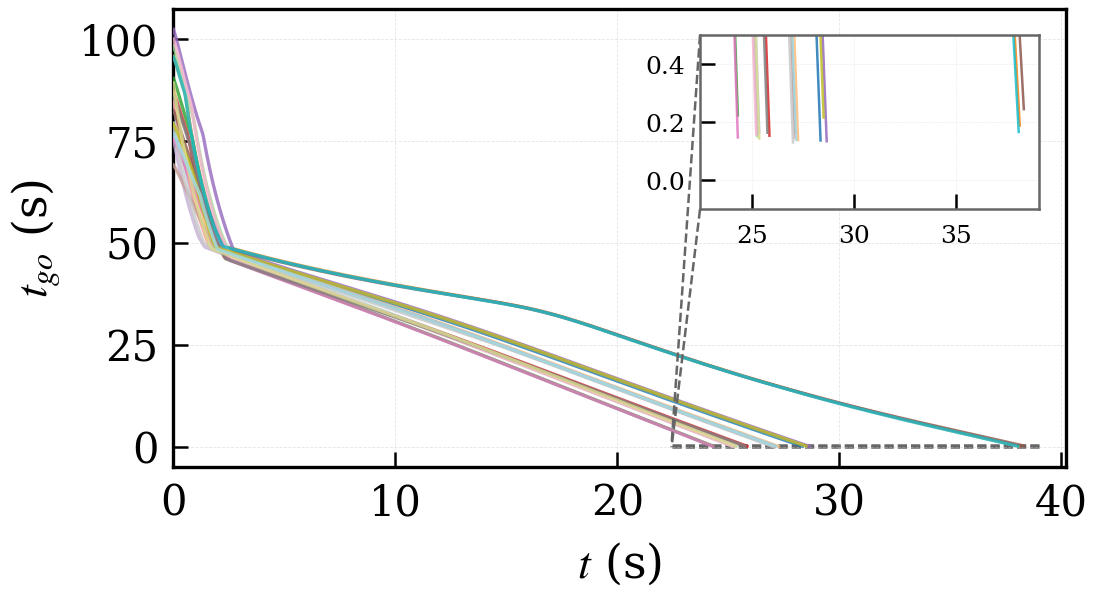
\includegraphics[width=3.2in]{mappo_sin_tgo.png}
%DIFDELCMD < %%%
\DIFdelendFL \DIFaddbeginFL 
\includegraphics[width=3.2in]{../new_sim_fig/figures_v10/pn/pn_sin_tgo.png}
\DIFaddendFL \caption{Time-to-go ($t_{go}$) profiles of the defending swarm using \DIFdelbeginFL \DIFdelFL{ART-MAPPO }\DIFdelendFL \DIFaddbeginFL \DIFaddFL{the PN baseline }\DIFaddendFL in
Case~2.\DIFdelbeginFL \DIFdelFL{Interceptors actively synchronize their remaining flight times despite the continuous high-G maneuvers of the targets.}\DIFdelendFL }
\DIFdelbeginFL %DIFDELCMD < \label{fig:case2_mappo_tgo}
%DIFDELCMD < %%%
\DIFdelendFL \DIFaddbeginFL \label{fig:case2_pn_tgo}
\DIFaddendFL \end{figure}

\DIFdelbegin \DIFdel{Consequently, the ultimate validation of ART-MAPPO's saturation strike capability under extreme dynamic conditions is explicitly presented in Fig.~\ref{fig:case2_time_sync}. Even against highly evasive sinusoidal targets, the maximum terminal arrival time difference ($\Delta t$)among the coordinated groups is strictly bounded to 0.30\,s. This exceptional synchronization quantitatively confirms the superiority of the ART-MAPPO framework in executing temporally coordinated saturation strikes in highly complex adversarial environments.
}%DIFDELCMD < 

%DIFDELCMD < %%%
\DIFdelend \begin{figure}[!ht]
\centering
\DIFdelbeginFL %DIFDELCMD < 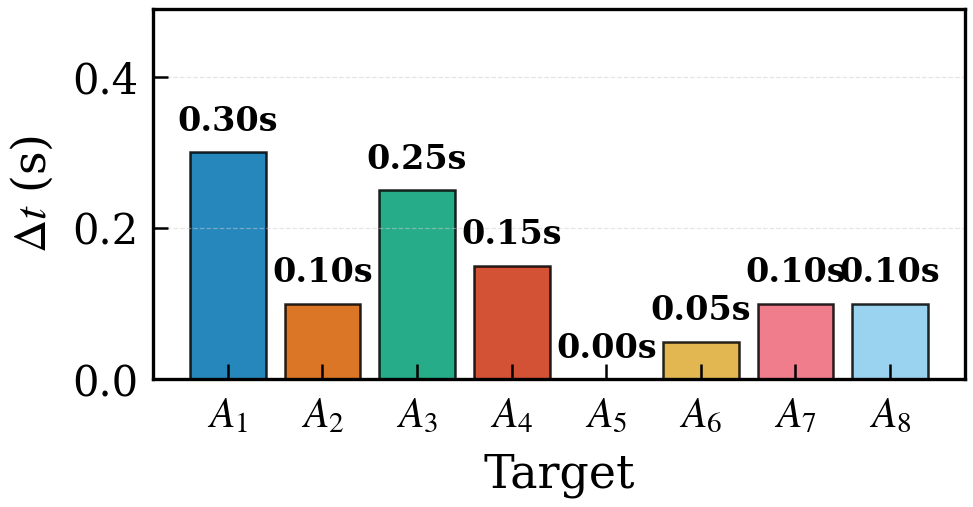
\includegraphics[width=3.0in]{mappo_success_sin_time_sync.png}
%DIFDELCMD < \caption{%%%
\DIFdelFL{Terminal arrival time differences $\Delta t$ for Case~2. The remarkably low variance ($\le 0.30$\,s) proves that ART-MAPPO preserves strict temporal synchronization even against continuous weaving targets.}%DIFDELCMD < \MBLOCKRIGHTBRACE
%DIFDELCMD < \label{fig:case2_time_sync}
%DIFDELCMD < %%%
\DIFdelendFL \DIFaddbeginFL 
\includegraphics[width=3.0in]{../new_sim_fig/figures_v10/pn/pn_sin_time_sync.png}
\caption{\DIFaddFL{Terminal arrival time differences $\Delta t$ within each PN interceptor group in
Case~2.}}
\label{fig:case2_pn_sync}
\DIFaddendFL \end{figure}
\DIFaddbegin \FloatBarrier
 \DIFaddend 

\subsection{Monte Carlo Statistical Analysis and Robustness}
\label{subsec:montecarlo}

To rigorously quantify the robustness of the proposed framework, 1000 independent Monte Carlo trials are conducted for each case. It is important to note that the statistical distributions presented in Fig.~\ref{fig:mc_boxplots} ($E_{co\text{-}time}$, $E_n$, $E_{miss}$, and $E_t$) are exclusively derived from the successful interception trials. Specifically, out of the 1000 trials in Case~1, ART-MAPPO and PN successfully intercepted the targets 987 and 944 times, respectively. In the highly dynamic Case~2, ART-MAPPO maintained a remarkable 971 successful interceptions, whereas the baseline PN succeeded only 175 times. 

\begin{figure}[!t]
\centering
\DIFdelbeginFL %DIFDELCMD < \subfloat[Case~1]{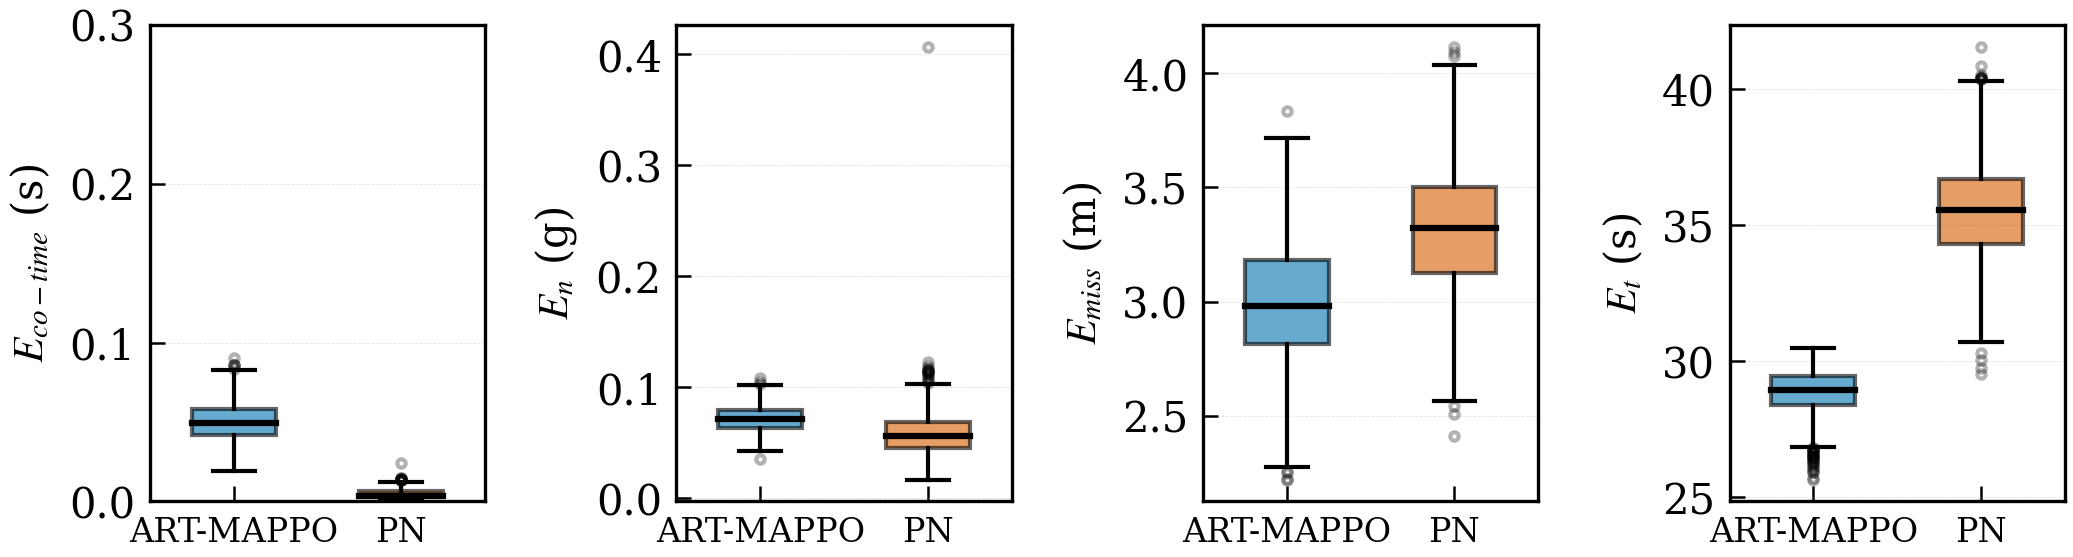
\includegraphics[width=3.5in]{nopn_mc_boxplot_compare.png}}%%%
\DIFdelendFL \DIFaddbeginFL \subfloat[Case~1]{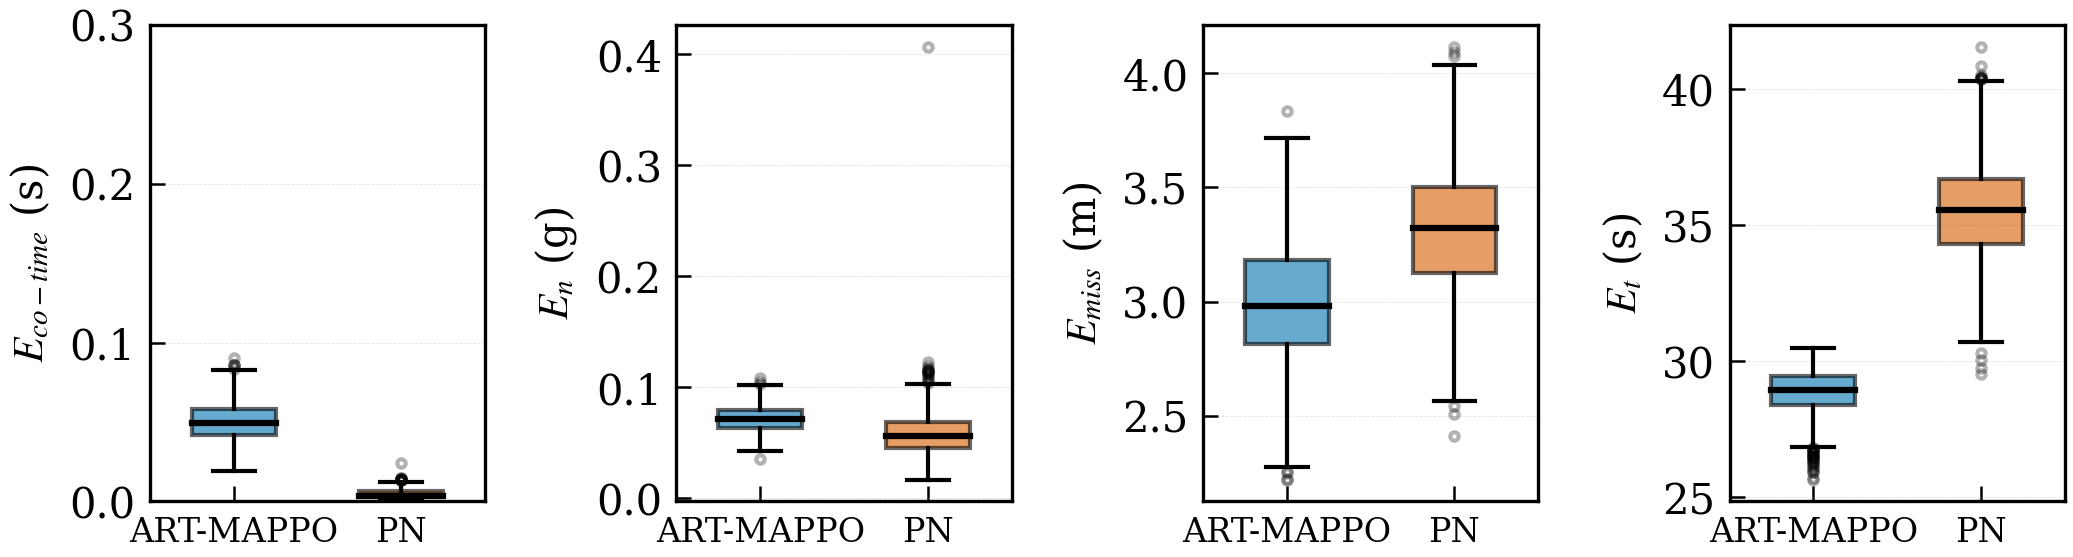
\includegraphics[width=3.47in]{nopn_mc_boxplot_compare.png}}\DIFaddendFL \\
\DIFdelbeginFL %DIFDELCMD < \subfloat[Case~2]{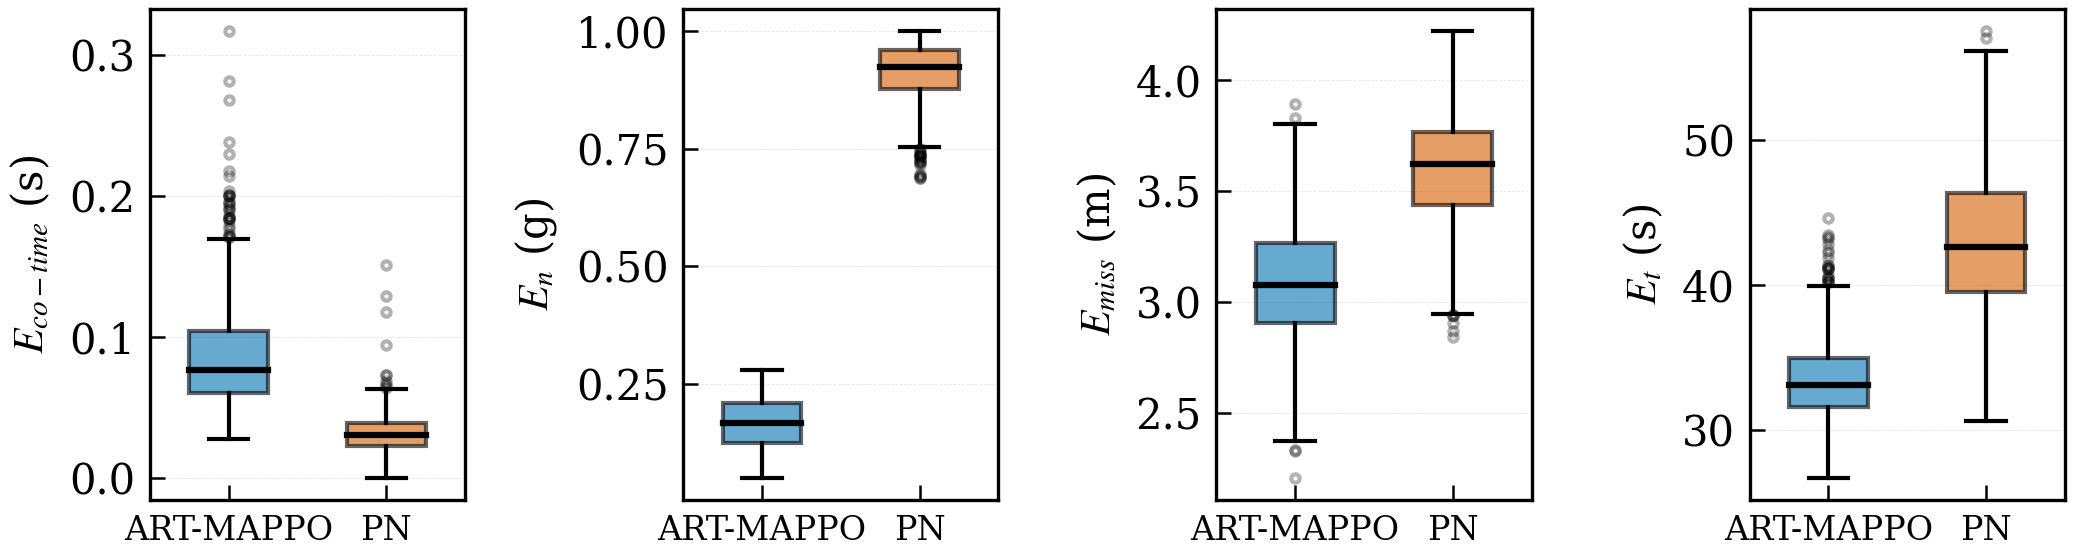
\includegraphics[width=3.5in]{sin_mc_boxplot_compare.png}}
%DIFDELCMD < %%%
\DIFdelendFL \DIFaddbeginFL \subfloat[Case~2]{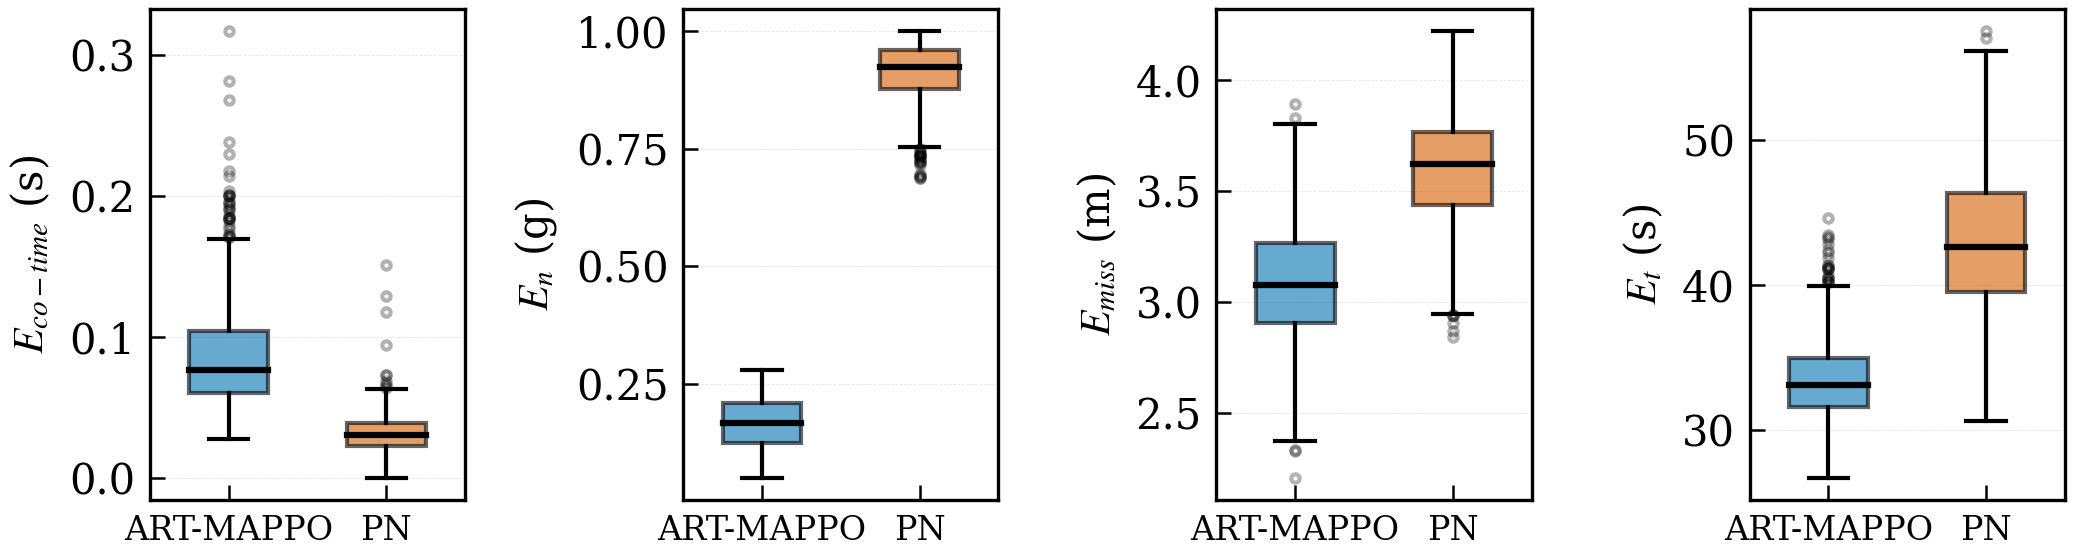
\includegraphics[width=3.47in]{sin_mc_boxplot_compare.png}}
\DIFaddendFL \caption{Boxplots of Monte Carlo trials comparing ART-MAPPO and PN (data derived from successful interceptions).}
\label{fig:mc_boxplots}
\end{figure}

Based on the statistical distributions, three key findings emerge:

\emph{(i) Interception reliability and precision.} The Interception Success Rates (ISRs) directly reflect the algorithms' adaptability to aggressive target maneuvers. While PN achieves a respectable 94.40\% against the evasive target (Case~1), its performance precipitously degrades to 17.50\% when facing the continuous weaving target (Case~2). Conversely, ART-MAPPO sustains exceptional ISRs of 98.70\% and 97.14\%, demonstrating profound robustness against continuous, high-frequency line-of-sight (LOS) oscillations. Furthermore, the $E_{miss}$ boxplots confirm that ART-MAPPO consistently achieves a lower median miss distance with a significantly narrower interquartile range (IQR), ensuring lethal precision even under worst-case initializations.

\emph{(ii) Terminal required overload and operational efficiency.} The metric $E_n$ denotes the terminal required normal overload, which is a critical constraint for flight safety. As depicted in the boxplots, ART-MAPPO's $E_n$ is tightly clustered around a safe median of $\approx0.08$\,g (Case~1) and $\approx0.20$\,g (Case~2). In stark contrast, particularly in Case~2, PN's $E_n$ distribution is heavily squeezed near the 1.0\,g upper bound. This exposes severe terminal actuator saturation, as PN struggles to reactively track the sinusoidal maneuvers. Additionally, ART-MAPPO strictly bounds the engagement duration ($E_t$) within a tight and predictable time window, reflecting superior forward energy management and rapid closure capabilities.

\emph{(iii) Robust temporal coordination.} The metric $E_{co\text{-}time}$ evaluates the temporal synchronization of the defending swarm. Across the successful Monte Carlo trials in both highly dynamic scenarios, ART-MAPPO maintains a median $E_{co\text{-}time}$ well below 0.10\,s. This consistently tight distribution confirms that the proposed algorithm can reliably shape the swarm's velocity profile to satisfy the strict temporal requirements for simultaneous saturation strikes, effectively neutralizing the risk of sequential piecemeal defeat.



%DIF < % ===========================================================
\section{Conclusion}
\label{sec:conclusion}

In this paper, the cooperative interception problem of UAV swarms against highly dynamic and
maneuverable attacking UAV swarms has been investigated, explicitly accounting for real-time
decision requirements, coordinated engagement effectiveness, and terminal overload risk.
The problem is formulated by jointly considering target assignment and cooperative guidance,
and an intelligent temporally coordinated interception framework is developed.
A fast IDBO-based target assignment mechanism enables efficient and accurate resource
allocation in dynamic environments.
The ART-MAPPO cooperative guidance strategy under the CTDE paradigm improves learning
stability and training efficiency in large-scale adversarial settings.
Extensive \DIFaddbegin \DIFadd{three-dimensional }\DIFaddend simulations demonstrate accelerated target assignment, enhanced interception
efficiency, improved interception success rates, and effective alleviation of terminal overload
saturation.

For future work, promising directions include cooperative interception under incomplete
information, dynamic target reassignment in unknown environments, time-constrained assignment
with explicit completion deadlines, and integration with realistic constraints such as
\DIFdelbegin \DIFdel{communication delays, }\DIFdelend limited bandwidth, \DIFaddbegin \DIFadd{aerodynamic coupling, }\DIFaddend and heterogeneous UAV capabilities.

%DIF <  ---- Bibliography ----
\bibliographystyle{IEEEtran}
\bibliography{cja-template}
\DIFaddbegin 

\appendices
\section{\DIFadd{Notation Table}}
\label{app:notation}

\DIFadd{Table~\ref{tab:notation} groups the main symbols by role. Symbols used only as temporary
indices inside a single equation are explained locally and omitted here.
}

\begin{table*}[!t]
\centering
\caption{\DIFaddFL{Grouped Notation Summary}}
\label{tab:notation}
\renewcommand{\arraystretch}{1.12}
\footnotesize
\begin{tabular}{@{}p{0.14\textwidth}p{0.32\textwidth}p{0.14\textwidth}p{0.32\textwidth}@{}}
\toprule
\DIFaddFL{Symbol }& \DIFaddFL{Description }& \DIFaddFL{Symbol }& \DIFaddFL{Description }\\
\midrule
\multicolumn{4}{l}{\emph{Sets, indices, and physical quantities}}\\
\DIFaddFL{$\mathcal D,\mathcal T$ }& \DIFaddFL{Defender and target sets. }&
\DIFaddFL{$N_D,N_A$ }& \DIFaddFL{Numbers of defenders and targets.}\\
\DIFaddFL{$i,j,k,t$ }& \DIFaddFL{Defender, target, assignment/episode, and guidance-step indices. }&
\DIFaddFL{$\mathcal N_i,\mathcal G_j$ }& \DIFaddFL{Communication neighbors of defender $i$ and defenders assigned to target $j$.}\\
\DIFaddFL{$\mathbf p_i,\mathbf v_i,V_i$ }& \DIFaddFL{Position, velocity vector, and speed of defender $i$. }&
\DIFaddFL{$\boldsymbol\ell_i,\gamma_{D_i},\theta_{D_i}$ }& \DIFaddFL{LOS unit vector, defender heading, and flight-path angle.}\\
\DIFaddFL{$d_i,t_{go,i}$ }& \DIFaddFL{Defender--target range and estimated time-to-go. }&
\DIFaddFL{$n_{x_i},n_{y_i},n_{z_i}$ }& \DIFaddFL{Axial, horizontal-normal, and vertical-normal load-factor commands.}\\
\midrule
\multicolumn{4}{l}{\emph{Target-assignment quantities}}\\
\DIFaddFL{$X_{ij},\mathbf X$ }& \DIFaddFL{Binary assignment variable and assignment matrix. }&
\DIFaddFL{$L_{\max}$ }& \DIFaddFL{Maximum defenders assigned to one target.}\\
\DIFaddFL{$p_{ij}^{\mathrm{int}}$ }& \DIFaddFL{Pairwise interception-probability proxy. }&
\DIFaddFL{$\boldsymbol\xi_i,\pi_{ij}$ }& \DIFaddFL{Latent and sigmoid-mapped target preferences.}\\
\DIFaddFL{$u_{ij},\chi_{ij}$ }& \DIFaddFL{Target-specific local utility and combat advantage. }&
\DIFaddFL{$b_{ij},\mathcal W_{i,j}$ }& \DIFaddFL{Target bid and defender $i$'s local winner set for target $j$.}\\
\DIFaddFL{$\Gamma^{(k)}$ }& \DIFaddFL{Pairwise assignment-consensus disagreement. }&
\DIFaddFL{$N_{\mathrm{pop}},K_{\mathrm{IDBO}}$ }& \DIFaddFL{Local population size and number of IDBO iterations.}\\
\midrule
\multicolumn{4}{l}{\emph{Learning quantities}}\\
\DIFaddFL{$\mathbf o_i^{(t)},\mathbf s_t$ }& \DIFaddFL{Local actor observation and joint critic state. }&
\DIFaddFL{$\mathbf H_i,\mathbf h_i,\mathbf g_i$ }& \DIFaddFL{Attention tokens, residual feature, and GRU state.}\\
\DIFaddFL{$\mathbf a_i^{(t)},\mathcal A$ }& \DIFaddFL{Three-dimensional load command and feasible action set. }&
\DIFaddFL{$\pi_\theta,V_\phi$ }& \DIFaddFL{Shared decentralized actor and centralized value function.}\\
\DIFaddFL{$\mathcal T_i,G_i^{(k)}$ }& \DIFaddFL{Training-time trust state and episodic return. }&
\DIFaddFL{$\varrho_t,\widehat A_t$ }& \DIFaddFL{PPO importance ratio and GAE advantage estimate.}\\
\DIFaddFL{$\varepsilon_{\mathrm{PPO}},c_{\mathrm{DC}}$ }& \DIFaddFL{PPO clipping factor and dual-clip parameter. }&
\DIFaddFL{$\delta_{\mathrm{KL}},\beta_{\mathrm{KL}}$ }& \DIFaddFL{Target KL divergence and adaptive KL penalty.}\\
\DIFaddFL{$r_i^{(t)},\gamma_{\mathrm{RL}}$ }& \DIFaddFL{Per-step reward and RL discount factor. }&
\DIFaddFL{$H_{\mathrm{ep}}$ }& \DIFaddFL{Episode horizon.}\\
\midrule
\multicolumn{4}{l}{\emph{Evaluation quantities}}\\
\DIFaddFL{$t_i^{\mathrm{arr}},\mathcal W_i$ }& \DIFaddFL{Arrival time and terminal measurement window. }&
\DIFaddFL{$E_{\mathrm{co\text{-}time}},E_n$ }& \DIFaddFL{Arrival-time dispersion and terminal-window load metric.}\\
\DIFaddFL{$E_{\mathrm{miss}},E_t$ }& \DIFaddFL{Terminal miss distance and coordinated engagement duration. }& & \\
\bottomrule
\end{tabular}
\end{table*}
 \DIFaddend 

\end{document}
